\documentclass[titlepage,letterpaper,final]{scrartcl}

\usepackage{scrindex}           % multiple index support using the "index" package
\usepackage{index}

%% THE FOLLOWING SHOULD CHANGE FOR A STABLE RELEASE:
\newcommand{\PISMREV}{revision \input{revision.tex}}
\newcommand{\PETSCREL}{3.1}
\newcommand{\PISMDOWNLOADMSG}{Get development version of PISM source code: \quad\texttt{svn co http://svn.gna.org/svn/pism/trunk pism-dev} \quad}

%\addtolength\topmargin{-.1in}
\addtolength\textheight{0.75in}
\addtolength{\oddsidemargin}{-.4in}
\addtolength{\evensidemargin}{-.4in}
\addtolength{\textwidth}{0.9in}
\newcommand{\normalspacing}{\renewcommand{\baselinestretch}{1.1}\tiny\normalsize}
\newcommand{\tablespacing}{\renewcommand{\baselinestretch}{1.0}\tiny\normalsize}
\normalspacing

\usepackage[usenames]{xcolor}

\usepackage{bm,url,xspace,verbatim}
\usepackage{amssymb,amsmath}
\usepackage[pdftex]{graphicx}


\usepackage{booktabs}           % better rules in tables
\usepackage{xtab}               % long (multi-page) tables

%% uncomment to see locations of index entries
% \proofmodetrue

\usepackage{underscore}

% this lets us avoid the scrartcl/hyperref conflict...
\let\ifvtex\relax

% hyperref should be the last package we load
\usepackage[pdftex,
                colorlinks=true,
                plainpages=false, % only if colorlinks=true
                linkcolor=blue,   % only if colorlinks=true
                citecolor=blue,   % only if colorlinks=true
                urlcolor=blue     % only if colorlinks=true
]{hyperref}[2010/03/30 v6.80u Hypertext links for LaTeX]

\newcommand{\ddt}[1]{\ensuremath{\frac{\partial #1}{\partial t}}}
\newcommand{\ddx}[1]{\ensuremath{\frac{\partial #1}{\partial x}}}
\newcommand{\ddy}[1]{\ensuremath{\frac{\partial #1}{\partial y}}}
\renewcommand{\t}[1]{\texttt{#1}}
\newcommand{\Matlab}{\textsc{Matlab}\xspace}
\newcommand{\bq}{\mathbf{q}}
\newcommand{\bU}{\mathbf{U}}
\newcommand{\eps}{\epsilon}
\newcommand{\grad}{\nabla}
\newcommand{\Div}{\nabla\cdot}

%% macros having to do with documentation for options; note these appear in the index

\newindex{default}{idx}{ind}{General Index}
\newindex{options}{odx}{ond}{PISM Command-line options}

\def\optsection#1{%
  \def\optindex##1{\index[options]{#1!##1}}
  \def\optseealso##1{\index[options]{#1|see{##1}}}
}

\optsection{FIXME}

% Use this to index option definitions:
\newcommand{\intextoption}[1]{\texttt{-#1}\optindex{\texttt{-#1}}}

\newcommand{\txtopt}[2]{\texttt{-#1} #2\optindex{\texttt{-#1} #2}}

\newcommand{\listopt}[1]{\txtopt{#1}{\emph{comma-separated list}}}
\newcommand{\fileopt}[1]{\txtopt{#1}{\emph{filename}}}
\newcommand{\timeopt}[1]{\txtopt{#1}{\emph{range or list}}}


\pdfinfo{
/Title (PISM User's Manual)
/Author (the PISM authors)
/Subject (Using PISM, a Parallel Ice-Sheet Model)
/Keywords (PISM ice sheet modeling)
}

\begin{document}
\graphicspath{{figs/}}

\begin{titlepage}
  \begin{center}
    {\huge\usekomafont{title} \emph{PISM}, a Parallel Ice Sheet Model:\\\medskip User's Manual}
    \vspace{1cm}

    {\Large The PISM Authors}
%    {\Large Constantine Khroulev \\ Ed Bueler \\ Andy Aschwanden \\ Jed Brown \\ Nathan Shemonski}
    \vspace{3cm}

    \includegraphics[width=3.in,keepaspectratio=true]{grn-grl-csurf}
    \vfill

    \small Support by email: \texttt{help\@@pism-docs.org}. 
    \medskip

    Manual date \today. Based on PISM \PISMREV.
    \medskip
    
    \PISMDOWNLOADMSG
  \end{center}
\end{titlepage}

\newpage
\phantom{bob}
\vspace{0.2in}
\begin{quote}
\textsl{Copyright (C) 2004--2011 The PISM Authors}
%\textsl{Copyright (C) 2004--2011 Constantine Khroulev and Ed Bueler and Andy Aschwanden and Jed Brown and Nathan Shemonski}
\medskip

\noindent \textsl{This file is part of PISM.  PISM is free software; you can redistribute it and/or modify it under the terms of the GNU General Public License as published by the Free Software Foundation; either version 2 of the License, or (at your option) any later version.  PISM is distributed in the hope that it will be useful, but WITHOUT ANY WARRANTY; without even the implied warranty of MERCHANTABILITY or FITNESS FOR A PARTICULAR PURPOSE.  See the GNU General Public License for more details.  You should have received a copy of the GNU General Public License\index{GPL (\emph{GNU Public License})} along with PISM; see \emph{\texttt{COPYING}}.  If not, write to the Free Software Foundation, Inc., 51 Franklin St, Fifth Floor, Boston, MA  02110-1301 USA}
\end{quote}
\vspace{0.2in}
\normalspacing

\centerline{\textsc{Authorship}}
\bigskip

\normalspacing
PISM is a joint project between developers at the University of Alaska (UAF) and in Anders Levermann's research group at the Potsdam Institute for Climate Impact Research (PIK).  The number of source code and script contributors, documentation authors, and source code authors is now large enough so that perhaps the best description is an alphabetical list, below.
\medskip

Users will reach the underlined UAF developers by mail to \texttt{help\@@pism-docs.org}.
\bigskip
\normalspacing

\renewcommand{\arraystretch}{1.3}
\begin{tabular}{ll}
\textbf{Torsten Albrecht} & ice shelf physics and numerics \\
\textbf{\underline{Andreas Aschwanden}} & scripts, visualization, SeaRISE-Greenland \\
\textbf{Jed Brown} & source code original author, SSA numerics, PETSc underpinnings \\
\textbf{\underline{Ed Bueler}} & principal investigator, numerics, verification, documentation \\
\textbf{Dani DellaGiustina} & regional modeling \\
\textbf{Marianne Haselhoff} & ice streams: physics and numerics\\
\textbf{Regine Hock} & surface mass and energy balance \\
\textbf{\underline{Constantine Khroulev}} & \begin{minipage}[t]{4in} source code primary author, input/output, software design, testing, documentation, most bug fixes \end{minipage} \\
\textbf{Craig Lingle}\index{People!Lingle, Craig} & original modeling choices, earth deformation, modeled-it-before-you-did \\
\textbf{Maria Martin} & SeaRISE-Antarctica \\
\textbf{David Maxwell} & SSA finite elements, python bindings \\
\textbf{Nathan Shemonski} & EISMINT-Greenland example \\
\textbf{Ricarda Winkelmann} & Antarctica processes, coupling, and modeling  \\
\textbf{Florian Ziemen} & bug fixes, sliding \\
\end{tabular}
\vfill

\newpage
\centerline{\textsc{Acknowledgements}}
\bigskip

\small
The NASA Modeling, Analysis, and Prediction program\index{Organizations!NASA!Modeling, Analysis, and Prediction Program} (grant \# NNX09AJ38G) supports the development of PISM from 2009 to 2013.  Development from 2002 to 2008 was supported by the NASA Cryospheric Sciences Program\index{Organizations!NASA!Cryospheric Sciences Program}.  The Snow, Ice, and Permafrost (SIP) group\index{Organizations!Geophysical Institute!Snow, Ice, and Permafrost group} at the Geophysical Institute is the home for the University of Alaska PISM developers; find us in Elvey 410D.  The Arctic Region Supercomputing Center\index{Organizations!Arctic Region Supercomputing Center (ARSC)} has provided significant computational resources and technical help in the development of PISM.

Dave Covey, Don Bahls, and Greg Newby have supported our hardware, software, and computations.  Bob Bindshadler, Sophie Nowicki, Jesse Johnson, and others in the SeaRISE group have assisted PISM development in many ways.  

Thanks to the many PISM users around the world, including

\begin{quote}
Tolly Adalgeirsdottir, Antje Fitzner, Nick Golledge, Marika Habermann, Tore Hattermann, Marianne Madsen, Malou Maris, Art Mahoney, Kent Overstreet, Sebastian Simonsen, Anne Solgaard, Ben Sperisen, Ward van Pelt, Martin Truffer, Shuting Yang, Ryan Woodard
\end{quote}

\noindent for helpful comments and questions on PISM and this \emph{Manual}.
\normalsize



\newpage
\setcounter{tocdepth}{3}
\small
\tableofcontents
\normalsize

\newpage


\section{Introduction}\label{sect:intro}

Welcome!  All information about PISM is online at
\begin{center}
  \href{http://www.pism-docs.org}{\t{www.pism-docs.org}}
\end{center}

See the \emph{Installation Manual} for how to download\index{PISM!download source code} the PISM source code and install it\index{PISM!install}, along with needed libraries.

This \emph{User's Manual} describes how to run PISM using certain publicly-available data for the Greenland ice sheet and the Ross ice shelf.  It illustrates how PISM's numerical approximations are verified.  It documents all the PISM options.  But it does not explain PISM internals, nor is it a guide for extending the functionality of PISM.

Users who want to understand how PISM works, extend PISM, and/or generally advance the science of ice sheets will need to go beyond what is described here.  For such users there is a \emph{C++ Class Browser}\index{PISM!\emph{C++ Class Browser (HTML)}}.  It gives a complete view of the class/object structure of the PISM source code.  It is the best tool for the job of modifying and supplementing PISM by writing derived classes.  See
\begin{center}
  \url{http://www.pism-docs.org/doxy/html/index.html}
\end{center}

\vspace{.4in}
  
\begin{center}
\includegraphics[width=3.5in,keepaspectratio=true]{rossquiver}
\end{center}

\vspace{.4in}

\large
\begin{center}
\framebox{\parbox{5.0in}{ \emph{WARNING}:\index{PISM!warning}  PISM is an ongoing project.  Ice sheet modeling is complicated and is generally not mature.  Please don't trust the results of PISM or any other ice sheet model without a fair amount of exploration.  Also, please don't expect all your questions to be answered here.  Write to us with questions at \href{mailto:help@pism-docs.org}{\texttt{help@pism-docs.org}}.} }
\normalsize
\end{center}
\normalsize


\clearpage\newpage

\section{Getting started}\label{sect:start}\ind{PISM!getting started}

In this section we give an extended example applying PISM to the Greenland ice sheet.  We use recent data sets provided by the Sea-level Response to Ice Sheet Evolution (\href{http://websrv.cs.umt.edu/isis/index.php/SeaRISE_Assessment}{SeaRISE}), a community-organized process to produce an upper bound of ice sheet contributions to sea level in the next 100--200 years.

The example in this section is a quick, hands-on first look at PISM.  It is not an in-depth tutorial, and many details of what is happening will only be explained later.  The sections on the older EISMINT-Greenland and EISMINT-Ross modeling cases, for instance, do a more complete job of explaining the ways users will need to preprocess not-so-clean input data and then make, and evaluate, modeling choices.

The PISM output figures in this section were produced using a supercomputer.  However, in order for the examples here to run on a typical workstation, a rather coarse $20\,\textrm{km}$ grid is used.  The purpose of PISM is to make much higher spatial resolution actually possible, but it requires large-scale \emph{parallel} processing.


\subsection{Install PISM}

See the \emph{Installation Manual}
   \begin{center}
     \href{http://www.pism-docs.org/dev/pdfs/installation-dev.pdf}{\t{www.pism-docs.org/dev/pdfs/installation-dev.pdf}}
   \end{center}
to install PISM.  Once installed, an executable \verb|pismr|, and several others, will be in the \verb|bin| subdirectory of the main PISM directory.  The main PISM directory might be at \verb|/home/username/pism-dev/|, for example.  The instructions below assume you start from that main PISM directory.  We also assume you are using a \verb|bash| shell or at least one that accepts \verb|bash| syntax.


\subsection{Obtain and preprocess the input data}

The NetCDF data file which we use for input is freely-available at, and is described by, this web page: 
\medskip

\centerline{\protect{\textbf{\url{http://websrv.cs.umt.edu/isis/index.php/Present_Day_Greenland}}}}
\medskip

\noindent The quickest way to get the file itself is to do

\verb|$ cd examples/searise-greenland|

\verb|$ ./preprocess.sh|

\noindent The script \verb|preprocess.sh|\footnote{\protect{This script requires \texttt{wget} and NCO (NetCDF Operators; \url{http://nco.sourceforge.net/})}.} downloads the ``master'' present-day data set and adjusts it to make it PISM-readable.\footnote{The script looks for \texttt{Greenland\_5km\_v0.93.nc}.  If a different version number is desired, edit the script to change the line ``\texttt{DATAVERSION=0.93}''.}

Preprocessing creates three NetCDF files from the master data, each of which has small ``metadata'' changes so that they can be read by PISM.  The metadata itself can be listed at the command line, or put in a text file, by \verb|ncdump -h|.  Two of the new files contain famous time-dependent paleo-climate records from ice core (GRIP; \verb|pism_dT.nc|) and seabed core records (SPECMAP; \verb|pism_dSL.nc|).

Any of these NetCDF files can be viewed with \verb|ncview| or other NetCDF visualization tools.  (See Table \ref{tab:NetCDFview} below.)  Application of \verb|pyNGL| tools to \verb|Greenland_5km_v0.93.nc| produced figures \ref{fig:sr-input1} and  \ref{fig:sr-input1}, for example.

\begin{figure}[ht]
\mbox{\includegraphics[width=2.5in,keepaspectratio=true]{sr-greenland-thk}
 \qquad\qquad\includegraphics[width=2.5in,keepaspectratio=true]{sr-greenland-prcp}}
\caption{The input present-day ice thickness (left; m) and present-day precipitation (right; m $\text{a}^{-1}$ ice equivalent) for SeaRISE-Greenland.  Figures produced with IDV}
\label{fig:sr-input1}
\end{figure}

\begin{figure}[ht]
\mbox{\includegraphics[width=2.5in,keepaspectratio=true]{sr-greenland-topg}
 \qquad\quad \includegraphics[width=2.5in,keepaspectratio=true]{sr-greenland-bheatflx}}
\caption{The input bedrock elevation (left; m) and geothermal flux (right; W $\text{m}^{-2}$) for SeaRISE-Greenland.  Figures produced with IDV}
\label{fig:sr-input2}
\end{figure}


\subsection{Run PISM}

We are ready to run PISM, but, perhaps even more than many unix programs, PISM allows \emph{a lot} of command-line options.  In fact, because it is an ice flow simulation program designed to handle many different ice sheets, shelves, and glaciers, the list of user-configurable flags and parameters is quite long.\footnote{We believe this is a feature not a bug.}  For a complete list of configuration flags and parameters see
\begin{center}
\url{http://www.pism-docs.org/dev/doxy/html/config.html}
\end{center}
Therefore it is wise to build a \emph{script} to run PISM with the correct options. 

Also, as explained in the rest of this \emph{User's Manual}, modeling ice sheets requires the integration of paleo-climatic and long-time-scale information into the model state, so our script is called ``\verb|spinup.sh|''.  The spin-up stage is the one which generally requires the most processor-hours, compared to a ``forecast'' stage.

To see what the SeaRISE-Greenland PISM run involves, do this:

\verb|$ PISM_DO=echo|

\verb|$ ./spinup.sh|

\noindent Setting the environment variable \verb|PISM_DO| in this way tells \verb|spinup.sh| just to print out the commands it is about to run, not do them.

Note that ``\verb|mpiexec -n 2 pismr|'' appears in the echo-ed PISM runs from \verb|spinup.sh|.  This means that the PISM executable \verb|pismr| is run in parallel on two processes (e.g.~cores on a smaller machine).  Note ``\verb|pismr|'' stands for the standard ``run'' mode of PISM, in contrast to more specific modes as described later.  Also, for the rest of this example, we assume you have a workstation with 8 cores, which is typical of 2010 resources.

The script \verb|spinup.sh| starts by ``bootstrapping.''  This means the creation, by heuristics and simplified models, of the kind of full initial conditions needed for the evolving, time-dependent model.  Specifically, the first 100 model year run with 8 processes will look like
\begin{verbatim}
mpiexec -n 8 pismr -ocean_kill -eta -skip 2 -boot_from pism_Greenland_5km_v0.93.nc \
  -Mx 76 -My 141 -Lz 4000 -Lbz 2000 -Mz 41 -Mbz 16 \
  -atmosphere searise_greenland -surface pdd -pdd_fausto \
  -y 100 -o g20km_pre100.nc
\end{verbatim}
The options describe a $76\times 141$ point grid in the horizontal, which is a 20 km grid.  There are also important choices about the vertical extent and resolution of the computational domain; more on those later.

Instead of typing-in the above PISM command with all its options, get the run going by

\verb|$ export PISM_DO=|

\verb|$ ./spinup.sh 8 >> out.spin20km &|

\noindent PISM will show what it is doing in the text (ASCII) file \verb|out.spin20km| while it runs in the background.  Using \verb|less| is good for watching a growing text file.  It will fairly quickly---within a minute---produce a very-early flow result in \verb|g20km_pre100.nc|.  Also \verb|g20km_climate-500a.nc| shows a movie of the simulated Greenland ice-sheet-model-inputs ``climate'', from 1500 to today, an important result to look at early because surface mass balance is (and must) be simulated for this kind of spinup.

The total run time for the complete 20km spinup, which models 125,000 model years with ``full physics'' of the SIA+SSA hybrid type (section \ref{sect:dynamics}) uses about 80 processor-hours.  

FIXME:  This run should take about one minute of real time. Next we generate a more credible enthalpy field. One way to do this is to have the enthalpy field and velocity field co-evolve according to the thermomechanical flow model while holding the upper ice surface stationary.  This is a continuation of ``bootstrapping''.  The effect is to create an enthalpy field which is approximately stationary with respect to advection and conduction.\footnote{The resulting enthalpy field is not a fully physical enthalpy field, however, because it comes from a steadiness assumption about the geometry of the ice sheet.  Said another way, it is a enthalpy field in equilibrium with a velocity field for which the surface kinematical equation \cite{Fowler} is \emph{not} satisfied.}  We create this enthalpy field by running for 50000 years\footnote{A longer run might be desirabe, but here we only wish to have a reasonable starting field. More about how to determine the length of a no-mass run can be found in...} with non-evolving surface.  The option \verb|-no_mass| turns off the map-plane mass continuity scheme, and thus any evolution of the surface.
\begin{verbatim}
$ mpiexec -n 4 pismr -ocean_kill -skip 2 -i g20km_pre100.nc \
  -atmosphere searise_greenland -surface pdd -pdd_fausto -no_mass -y 50000 \ 
  -extra_file ex_g20km_steady.nc -extra_vars enthalpybase,temppabase \ 
  -extra_times 0:250:50000 -o g20km_steady.nc
\end{verbatim} This takes about 1 hour (4 processor hours). Before we proceed with the actual paleo-climate forcing, we add another short smoothing run:
\begin{verbatim}
$ mpiexec -n 4 /pismr -ocean_kill -skip 2 -i g20km_steady.nc \
  -atmosphere searise_greenland -surface pdd -pdd_fausto \
  -y 100 -o g20km_SIA.nc
\end{verbatim}



%%%%  OLD




\subsection{Handling NetCDF files}\label{subsect:nctoolsintro}  At a superficial level, \verb|pismr| is just a program which takes one or more NetCDF files as input, does some computation, and produces one or more NetCDF files as output.  The user is in charge of creating NetCDF input files containing data on ice sheets worth modeling\footnote{See the section \ref{sec:bootstrapping-format} and table \ref{tab:modelhierarchy} for a hint about data necessary for modeling.}, and extracting some meaning from the NetCDF output files.

The most basic tools for converting NetCDF files to and from a standard text representation are called \verb|ncdump| and \verb|ncgen|.  A glance at Unix \verb|man| pages for these tools might be wise at this time.

As suggested earlier, we regularly use \verb|ncview| to look at NetCDF files.  The NetCDF tools most frequently used by the PISM developers are shown in Table \ref{tab:NetCDFview}.  This website gives additional NetCDF-related tools:

\centerline{ \href{http://www.unidata.ucar.edu/software/netcdf/docs/software.html}{\t{www.unidata.ucar.edu/software/netcdf/docs/software.html}} } 

\newcommand{\netcdftool}[1]{#1\ind{NetCDF!tools!#1}}
\begin{table}[ht]
\caption{Some tools for viewing and modifying NetCDF files.}\label{tab:NetCDFview} 
\small
\begin{tabular}{@{}llll}\hline
\textbf{Tool} & \textbf{Site} & \textbf{Function}\\ \hline
\netcdftool{\texttt{ncdump}} & \emph{included with any NetCDF distribution} & dump binary NetCDF as \texttt{.cdl} (text) file \\
\netcdftool{\texttt{ncgen}} & \emph{included with any NetCDF distribution} & convert \texttt{.cdl} file to binary NetCDF \\
\netcdftool{\texttt{ncview}} & \href{http://meteora.ucsd.edu/~pierce/ncview_home_page.html}{\texttt{meteora.ucsd.edu/$\sim$pierce}} & quick graphical view \\
\netcdftool{IDV} & \href{http://www.unidata.ucar.edu/software/idv/}{\t{www.unidata.ucar.edu/software/idv/}} & more complete visualization \\
\netcdftool{Paraview} & \href{http://www.paraview.org}{\t{www.paraview.org}} & powerful open-source parallel visualization \\
\netcdftool{NCL} &  \href{http://www.ncl.ucar.edu}{\t{www.ncl.ucar.edu}} & NCAR Command Language, open-source\\
\netcdftool{PyNGL} &  \href{http://www.pyngl.ucar.edu}{\t{www.pyngl.ucar.edu}} & Python version of NCL, open-source\\
\netcdftool{VisIt} & \href{http://visit.llnl.gov}{\t{visit.llnl.gov}} & advanced parallel visualization \\
\netcdftool{NCO}\ind{NCO (NetCDF Operators)} & \href{http://nco.sourceforge.net/}{\t{nco.sourceforge.net/}} & ``NetCDF Operators'': manipulations \\
\quad  & & \quad at command line
\end{tabular}
\normalsize
\end{table}


%%% Local Variables: 
%%% mode: latex
%%% TeX-master: "manual"
%%% End: 




\clearpage
\newpage
\section{Ice dynamics, the PISM view}\label{sect:dynamics}

\subsection{PISM design principles}\index{PISM!principles}  This section gives an overview of ice dynamics models in PISM.  First, some organizing principles:
\begin{enumerate}
\item source code should be open, free, and work well with other free software tools,
\item science is better if done with publicly-available data,
\item numerical methods should be verifiable (i.e.~compare to exact solutions of the modeled equations),
\item shallow models are (currently) the most effective at whole ice sheet scale,
\item comparing results from a hierarchy of ice dynamics simplifications is more valuable than getting them from any particular model equations,
\item everything computed diagnostically (instantaneously) should be available prognostically (i.e.~it can evolve in time), and
\item climate inputs should affect ice dynamics by a well-defined interface.
\end{enumerate}

\noindent We do not claim to follow these principles perfectly, but principle 1 is illustrated by our existence and principle 2 by examples in sections \ref{sect:start}, \ref{sec:eismint-greenland}, and \ref{sect:ross}.  Principle 3 is addressed in section \ref{sect:verif}.  Principles 4, 5, 6, and 7 are addressed next.


\subsection{Two main shallow models, SIA and SSA}\index{PISM!SIA}\index{PISM!SSA}  At each time-step of a typical PISM run, the geometry, temperature, and basal strength of the ice sheet are included into stress (momentum) balance equations to determine the velocity of the flowing ice.   The ``full'' stress balance equations, namely the (non-Newtonian) Stokes model for slowly-flowing fluids \cite{Fowler}, are themselves an inertia-free approximation of the conservation of momentum equations.  Even though PISM does not solve this ``full'' model, it can numerically solve two different shallow approximations which are suited to the situations in large ice sheet and ice shelf systems:
\begin{itemize}
\item the non-sliding shallow ice approximation (SIA)\index{SIA (shallow ice approximation)} \cite{Hutter}, also called the ``lubrication approximation'' \cite{Fowler}, which describes ice as flowing by shear in planes parallel to the geoid, with a strong contact of ice base to bedrock, and
\item the shallow shelf approximation (SSA)\index{SSA (shallow shelf approximation)} \cite{WeisGreveHutter}, which describes a membrane-type flow of floating ice \cite{Morland}, or grounded ice which is sliding over a weak base \cite{MacAyeal,SchoofStream}.
\end{itemize}
PISM solves both the SIA and SSA equations in parallel.  Time-stepping solutions of the mass continuity and energy conservation equations are possible when using each model.

The SIA\index{SIA (shallow ice approximation)!applicability} equations are, as a rule, easier and quicker to numerically solve than the SSA, and they are also easier to parallelize.\index{parallelization!relative ease of, between SIA and SSA}  They describe the shear as a local function of the driving stress of classical glaciology \cite{Paterson}.  They can confidently be applied to those grounded parts of ice sheets for which the basal ice is frozen to the bedrock, or minimally sliding, and for which the bed topography is relatively slowly-varying in the map-plane \cite{Fowler}.  These characteristics apply to the majority \emph{by area} of the Greenland and Antarctic ice sheets.  We recommend solving the SIA with a completely \emph{non-sliding} base because the ad~hoc addition of ``sliding laws''\index{SIA (shallow ice approximation)!sliding laws} into the SIA stress balance, and especially schemes which ``switch on'' at the pressure-melting temperature \cite{EISMINT00}, have bad continuum and numerical modeling consequences \cite[appendix B]{BBssasliding}.

The SSA\index{SSA (shallow shelf approximation)!applicability} equations, by contrast, can confidently be applied to large floating ice shelves, which have small depth-to-width ratio and negligible basal resistance \cite{Morland,MorlandZainuddin}.  The flow speeds in ice shelves are frequently an order-of-magnitude higher than in the non-sliding, grounded parts of ice sheets, and this speed contrast is easily seen in comparing the solutions of SIA and SSA models.

Terrestrial ice sheets also have fast-flowing grounded parts, however, called ``ice streams'' or ``outlet glaciers'' \cite{TrufferEchelmeyer}.  Such features appear at the margin of, and sometimes well into the interior of, the Greenland \cite{Joughinetal2001}\index{Ice Sheets!Greenland ice sheet} and Antarctic \cite{BamberVaughanJoughin}\index{Ice Sheets!Antarctic ice sheet} ice sheets.  Describing these faster-flowing grounded parts of ice sheets requires, at least, something more than the non-sliding SIA because adjacent columns of ice which have different amounts of basal resistance exert strong ``longitudinal'' or ``membrane'' stresses \cite{SchoofStream} on each other.  One might use the full Stokes equations, or a ``higher-order'' model (which still uses some shallow approximations \cite{Blatter,Pattyn03}), but this immediately leads to a resolution-versus-stress-inclusion tradeoff because the amount of computation per map-plane grid location is so much higher in these models.  Also, with any stress balance model one must still specify an appropriate sliding boundary condition, and uncertainty in this boundary condition may (and usually does) dominate the modeling error made by not including higher-order stresses in the balance.

If the fast-flowing grounded ice is sufficiently shallow, in the usual aspect-ratio sense, then the SSA model can be applied.  The best-known combination of the SSA model with a choice of basal resistance model is the Siple Coast (Antarctica) ice stream model by MacAyeal\index{People!MacAyeal, Doug} \cite{MacAyeal}, who used a linearly-viscous model for the underlying till.  A free boundary problem with the same (SSA) balance equations is the Schoof\index{People!Schoof, Christian} \cite{SchoofStream} model of ice streams, using a plastic (Coulomb) sliding relation.  In this model ice streams appear where there is ``till failure'' \cite{Paterson}---the basal shear stress exceeds the yield stress imposed as a boundary condition---and the location of ice streams is not imposed in advance.

As noted, both the SIA and SSA models are \emph{shallow} approximations.  More precisely, these model equations are derived from the Stokes equations by different small-parameter arguments, both based on a small depth-to-width ratio for the ice sheet.  Both models, and ``higher order'' models as well, approximate the pressure as hydrostatic.  For the small-parameter argument in the SIA case see \cite{Fowler}.  For the corresponding SSA argument, see \cite{WeisGreveHutter} or the appendices of \cite{SchoofStream}.  Schoof and Hindmarsh \cite{SchoofHindmarsh} have analyzed the connections between these shallowest models and ``higher order'' models, while \cite{GreveBlatter2009} discusses ice dynamics and stress balances comprehensively.

In PISM the SSA may be used as a ``sliding law'' for grounded ice which is already modeled everywhere by the non-sliding SIA \cite{BBssasliding}.  In brief, our concept for grounded ice is that, in addition to including shear in planes parallel to the geiod, we must balance the membrane stresses which become important anywhere there is significant sliding, and this inclusion is especially important when there are changes in basal strength, both spatial and temporal.  The more traditional use of ``sliding laws'' in pure-SIA models does not incorporate this basic physical truth \cite{Fowler01}.

The resulting ``SIA+SSA hybrid'' model is recommended by the PISM developers for most whole ice sheet modeling purposes because it seems to be a good compromise given currently available data and computational power (see \cite{BKAJS,Martinetal2010TCD,Winkelmannetal2010TCD}, for example).  This ``sliding law'' role for the SSA is in addition to its more obvious role in ice \emph{shelf} modeling, and so the SSA plays both roles in a PISM whole ice sheet model if there are large floating ice shelves--- as in Antarctica \cite{Martinetal2010TCD,Winkelmannetal2010TCD}.

By default, PISM does not numerically solve the SSA because any such solution must go with a conscious user choice about basal strength.  The user must both use a command-line option to turn on the SSA (section \ref{subsect:ssacontrol}) and also make choices in input files and runtime options about basal strength (section \ref{subsect:basestrength}).


\subsection{A hierarchy of simplifying assumptions for grounded ice flow}
\label{sec:model-hierarchy}\index{PISM!hierarchy of simplifying assumptions}

Table \ref{tab:modelhierarchy} describes a hierarchy of models, listed in order of increasing effectiveness in modeling grounded ice sheets with fast flow features.  This is also the order of increasing need for data to serve as boundary and initial conditions, an important consideration for the scientific user.

As an additional row for such a table, one might list ``full Stokes''.  That stress balance is \emph{not} planned for PISM at any time, however, as its numerical solution requires a fundamentally different computational architecture.

It makes sense to also talk about an \emph{ice shelf} model hierarchy, and even about a special hierarchy of models for the transition from grounded to floating ice \cite{SchoofMarine1}, but this would take us too far afield.  Currently, ice shelves should always be modeled by the SSA equations in PISM.  See section \ref{sect:ross}.

Although it begins to expose the internals of PISM, we think it is also helpful to see the implemented stress balances as PISM software components (C++ classes).  Figure \ref{fig:stressbalance} shows that the sequence of actions taken by SIA-only, SSA-only, and SIA+SSA hybrid models is, in some sense, the same: a membrane stress solution first, a distribution of vertical shear in the column of ice second, and a use of incompressibility to compute the vertical component of the velocity third.  The nonsliding SIA-only model has a degenerate first step and the SSA-only model has a degenerate second step.  The hybrid model described by Pollard and deConto \cite{PollardDeConto}, for another example, would add the shear in the column in a different manner (than in the current implementation, following \cite{BBssasliding,Winkelmannetal2010TCD}).

\newenvironment{tightlist}{\begin{itemize}  \vspace{-0.15in}\addtolength{\itemsep}{-0.5\baselineskip} } {\vspace{-0.1in} \end{itemize}}

%\newcommand{\nolist}[1]{\begin{tightlist} \item[] [\emph{#1}] \end{tightlist}}
\newcommand{\nolist}[1]{[\emph{#1}] \vspace{0.1in}}

\begin{table}[ht]
\caption{Hierarchy of current and planned flow models in PISM, for the grounded parts of ice sheets, from most to fewest simplifying assumptions \emph{and} from least to greatest need for boundary data.  The \emph{italicized} models are planned for future versions of PISM but are not implemented in \texttt{stable0.3}.}\label{tab:modelhierarchy} 
\small\medskip
\begin{tabular}{p{0.22\linewidth}p{0.40\linewidth}p{0.32\linewidth}}\hline
\textbf{Model} & \textbf{Assumptions} & \textbf{Required data} \\ \hline
\vspace{2mm}  \emph{perfectly-plastic ice} \small & \vspace{2mm}\emph{steady state}; ice has shear stresses at or below a pre-determined ``yield stress''; requires location of ice sheet margin  \vspace{2mm} & \vspace{2mm} \begin{tightlist} \item bed elevation\end{tightlist} \\
\emph{balance velocities} \small & \emph{steady state}; ice flows down surface gradient \cite{JoughinetalGrBal97} & \nolist{same as above, plus:}  \begin{tightlist} \item surface mass balance \item initial ice thickness \end{tightlist} \\
\textsc{isothermal SIA} & non-sliding lubrication flow, fixed softness \cite{BLKCB,EISMINT96} & \nolist{same as above, but time-dependence is allowed} \\
\textsc{thermo-coupled SIA} & non-sliding lubrication flow, temperature-dependent softness \cite{BBL,EISMINT00} & \nolist{same as above, plus:} \begin{tightlist} \item surface temperature \item geothermal flux \end{tightlist} \\
\textsc{polythermal SIA} & same, but allowing $>0$ liquid water in temperate ice; conserves energy better \cite{AschwandenBlatter,Greve} \vspace{2mm} & \nolist{same as above} \\
\textsc{SIA + SSA hybrid} & SSA as a sliding law for thermo-coupled SIA \cite{BBssasliding}; polythermal is the default & \nolist{same as above, plus:} \begin{tightlist} \item basal layer (``till'') strength \end{tightlist} \\
\emph{Blatter-Pattyn} \small & ``higher-order'', bridging stresses \cite{Blatter,Pattyn03,SchoofCoulombBlatter} & \nolist{same as above} \\ \hline
\end{tabular}
\normalsize
\end{table}


\subsection{Evolutionary and diagnostic modeling} \label{subsect:basicmodes}\index{PISM!evolution run}\index{PISM!diagnostic run}    The main goal of a numerical ice sheet model like PISM is to be a dynamical system which evolves over time as similarly as possible to the modeled ice sheet.  Such a goal assumes one has the right climate inputs and parameter choices at each time step.  For predictive purposes, it also assumes one has the right initial conditions, adequately describing the present state of the ice sheet.  This last assumption is rarely satisfied.  Instead, heuristics must be used to minimally-initialize an ice sheet model, before a possible stage of paleo-climate driven spinup; see section \ref{sect:boot}.

Underlying an ice sheet model like PISM are evolution-in-time partial differential equations.  PISM solves these by taking small time steps.  ``Small'' time steps vary from hundredths to many model years, depending primarily on grid resolution and modeled ice flow speed.  Time steps are chosen adaptively in PISM, according to the stability criteria of the several numerical methods.

However, much ice flow modeling, especially of streams and shelves, uses only instantaneous ``diagnostic'' solution of the partial differential equations which determine the velocity field.  The models in PISM can produce such ``instantaneous'' velocity fields because of the slowness of the ice, in the sense that inertia can be neglected in the stress balance \cite{Fowler}.  The goal of a ``diagnostic run'' is usually to compute this velocity field, especially its observable surface values.  For example, a diagnostic run might be the ``forward model'' step in inverting surface velocities for basal strength\dots but that is beyond the scope of this \emph{Manual}.

Sections \ref{sec:eismint-greenland} and \ref{sect:ross} are examples illustrating evolutionary and diagnostic modeling modes of PISM.  The first of these describes time-stepping evolution models for the Greenland ice sheet, while the second describes a diagnostic SSA model for the Ross ice shelf.


\begin{figure}
  \centering
  \includegraphics[width=6in]{stressbalance}
  \caption{The SIA-only, SSA-only, and SIA+SSA hybrid models represent different ``routes'' through stress balance PISM components.  In each case the inputs are ice geometry and boundary stresses, and the final output is a three-dimensional velocity field within the ice.}
  \label{fig:stressbalance}
\end{figure}


\subsection{Climate inputs, and their interface with ice dynamics}
\label{sec:climate-inputs}  

Because PISM's job is to approximate ice flow, its ``world view'' is centered around ice dynamics.  The discussion of boundary conditions, in this \emph{Manual} is necessarily ``ice-centric'' in our description here, but there is no constraint on the nature of, or completeness of, climate models which could be coupled to PISM.  This section applies the PISM organizing principle above (section \ref{sect:dynamics}): \emph{climate inputs affect ice dynamics by a well-defined interface}.

Figure~\ref{fig:climate-inputs} illustrates that any PISM ice sheet model has an interface (green) to a surface processes layer containing snow, firn, and liquid (or refrozen) runoff, and to the ocean (blue) if there is floating ice.  The surface processes layer might be very simple.  If it is ``owned'' by the PISM model then there is an additional interface (red) to the atmosphere above.  The interface to the surface layer is assumed in PISM to cover the whole surface of the ice, including ablation areas and even ice-free land.  Table \ref{tab:ice-dynamics-bc} lists fields which are needed as boundary conditions at the interfaces.

\begin{figure}
  \centering
  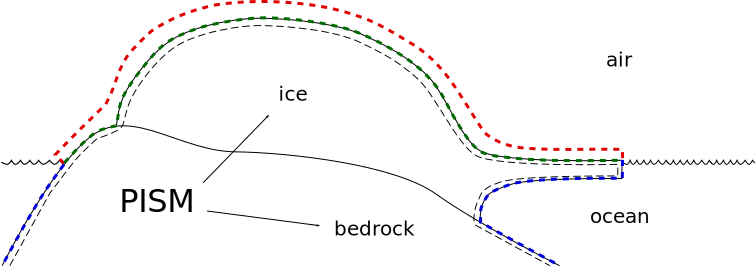
\includegraphics[width=6in]{figs/climate-cartoon.pdf}
  \caption{PISM's view of interfaces between an ice sheet and the outside world}
  \label{fig:climate-inputs}
\end{figure}

\begin{table}[h]
  \centering
  \begin{tabular}{p{0.35\linewidth}p{0.55\linewidth}}\\
    \hline
    \textbf{Boundary} & \textbf{Necessary conditions}\\
    \hline
    Top ice surface (below firn) (\textcolor{green}{green})& Ice temperature (or enthalpy) and mass flux into the ice\\
    Bottom surface of the thermal bed layer (not shown) & Geothermal flux\\
    Ice shelf basal surface (\textcolor{blue}{blue})& Mass flux into the ocean and ice boundary temperature\\
   \hline
  \end{tabular}
  \caption{Boundary conditions required by PISM's ice dynamics core; see figure
  \ref{fig:climate-inputs}}
  \label{tab:ice-dynamics-bc}
\end{table}

Regarding the base of the ice, as described in section \ref{subsect:beddef} PISM also includes an optional bed deformation component approximating the movement of the Earth's crust and upper mantle in response to changing ice load.   Furthermore the temperature of the layer of bedrock in contact with grounded ice is included in the conservation of energy model.  In this sense everything below the black dashed line (i.e.~ice and bedrock) is ``owned'' by PISM.  This fact adds two more boundary interfaces for the ice dynamics core: sub-ice-shelf/ocean (shown in blue) and the bottom of the bedrock thermal layer (not shown).

The PISM ice dynamics core would like to be able to get these fields directly from observations or measurements, or directly from a GCM.  In many realistic modeling situations, however, PISM code must be used for all or part of the surface processes modeling necessary to provide the ice-dynamics core with the ``right'' fields.  Due to differences in model resolutions and required down-scaling, this need for some PISM-based boundary-processes modeling includes cases where PISM is coupled to a GCM.  In the kind of ``offline'' runs described in this \emph{Manual}, boundary processes are modeled, even if trivially.

Thus, to be able to use the data that \emph{is} available, an ice-sheet model has to
have additional components that are responsible for modeling surface (snow)
processes or sub-shelf/ocean interaction.  These components might be very minimal, merely turning data that we already have into data in the right units and with the right metadata, so that PISM knows what to do with it, for example.

Thus we have PISM's design: the ice-dynamics-and-earth-deformation PISM
core does not contain any parameterization or other model for boundary mass or
energy balance.  These boundary parameterizations and models are present in the PISM source code, however, as instances of \emph{PISMComponent} classes.  This simplifies customizing and debugging PISM's climate
inputs, promotes code reuse.  Moreover, it isolates the code that needs to be changed to
couple PISM to a climate model.

Users wishing to customize PISM's climate inputs should see the \emph{PISM
  Source Browser}, e.g.~at
\url{http://www.pism-docs.org/doxy/html/index.html} and the documentation
of \emph{PISMSurfaceModel}, \emph{PISMAtmosphereModel} and
\emph{PISMOceanModel} therein.  Also, section \ref{sec:eismint-greenland} describes a
modeling example using a non-standard air temperature parameterization. Looking
at \texttt{pgrn.cc} and \texttt{pgrn_atmosphere.cc} may be a reasonable
start.

Note that figure~\ref{fig:climate-inputs} includes an interface that was not
mentioned yet, the one between the surface layer and the air (red dashed line).
Unlike the ones listed in table~\ref{tab:ice-dynamics-bc}, this interface
\emph{may not even be present in some PISM configurations:} the ice dynamics
core of PISM only ``knows'' about mediums bordering ice and bedrock. A pair
consisting of a \emph{PISMSurfaceModel} and a \emph{PISMOceanModel} may be
hiding anything from a nearly trivial parameterization of ice surface
temperature plus surface and sub-shelf mass fluxes to a GCM of great
complexity.

Figure~\ref{fig:climate-input-data-flow} illustrates the corresponding data
flow \emph{into} the PISM core; the data flow in the other direction depends on
particular modeling choices.

This figure requires an explanation: a ``modifier'' in this context is an
adjustment of climate inputs that can be used with different climate
choices.  Using ice-core-derived air temperature offsets to model the space-time distribution of paleo surface temperature is an example.  Note that PISM has a generic ``forcing'' mechanism that can be paired with another model. Please see section \ref{sec:boundary-models} for
a list of climate components included in PISM source code and other details.

\begin{figure}
  \centering
  \includegraphics[width=5in]{figs/data-flow.pdf}
  \caption{PISM climate input data flow. Colored arrows correspond to interfaces in
    figure \ref{fig:climate-inputs}.}
  \label{fig:climate-input-data-flow}
\end{figure}

Why describe this structure here? On the one hand, some users may be interested
in coupling PISM to other models. On the other hand, the PISM authors do not
claim expertise in modeling atmosphere, ocean, or even snow processes.   So the
separation has a code-reliability purpose. Indeed PISM users need to know that
they are ultimately responsible for providing the climate inputs they intend.
The auxiliary tool \texttt{pclimate}, described in subsection
\ref{subsect:pclimate}, is intended to help users observe the climate inputs
they have chosen, without involving ice dynamics at all.

\clearpage
\newpage
\section{Initialization and bootstrapping}
\label{sect:boot}  

\subsection{``Initialization from a saved model state''}  This phrase\index{initialization!from saved model state} has a simple meaning in PISM.  If a previous PISM run has saved a NetCDF file using ``\texttt{-o}'' then that file will contain complete initial conditions for continuing the run.  The output file from the last run can be loaded with ``\texttt{-i}'': \index{executables!\texttt{pisms}}

\begin{verbatim}
$ pisms -eisII A -y 100 -o foo.nc
$ pisms -eisII A -i foo.nc -y 100 -o bar.nc
\end{verbatim}
\smallskip

Note that simplified-geometry experiments (section \ref{sect:simp}) and verification tests (section \ref{sect:verif}) do not need input files at all because they initialize from formulas in the source code.  They can be continued from saved model states using \texttt{-i}.  As in the above example, however, specifying the simplified geometry experiment or verification test \emph{is} necessary, so that the run can continue with the climate inputs for that experiment or test.  For example, based on the above \texttt{pisms} runs, it is valid to do ``\texttt{\$ pismr -i foo.nc -y 100 -o bar.nc ...}'' but the climate and other parameters us PISM default values, and thus are not (necessarily) the values specified in EISMINT II.

As a technical but important note about saved states, a PISM run with \texttt{-ssa_floating_only} or \texttt{-ssa_sliding}
also saves the last SSA velocities to the output file, in variables 
\texttt{ubar_ssa} and \texttt{vbar_ssa}. The presence
of these velocities adds efficiency in restarting.  If you want a PISM restart to
ignore these velocities use \texttt{-dontreadSSAvels}.

\subsubsection*{\texttt{-i} file format}
PISM produces\footnote{Or, more accurately, attempts to produce; please let us know about violations you come across.} CF-1.4 compliant NetCDF\index{PISM!NetCDF file format}\index{NetCDF} files.  The easiest way to learn the output format \emph{and} the \texttt{-i} format is to do a simple run and then look at the metadata in the resulting file, like this:
\begin{verbatim}
$ pisms -eisII A -y 10 -o foo.nc
$ ncdump -h foo.nc | less
\end{verbatim}

Note that variables have a \texttt{pism_intent}\index{PISM!\texttt{pism_intent} attribute} attribute.  When that attribute is \texttt{diagnostic}, the variable can be deleted from the file without affecting whether PISM can use it as a \texttt{-i} input file.  Variables with \texttt{pism_intent} = \texttt{model_state}, by contrast, must be present for use with \texttt{-i}.

Regarding the automatically produced time variable, which has a \texttt{units} attribute like \texttt{"years since 1-1-1"}, note that CF metadata conventions require using a reference date in the units string of a time (\texttt{t}) variable.  PISM completely ignores this reference date.


\subsection{``Bootstrapping''} 
\optsection{Bootstrapping}
\optseealso{Grid}

This phrase\index{bootstrapping}\index{initialization!by bootstrapping} means starting a modeling run with less than sufficient data, and letting the model fill in needed values according to heuristics.  These heuristics are applied before the first time step is taken, so they are part of an initialization process.  Bootstrapping uses the option \fileopt{boot_file}.

The need for an identified stage like ``bootstrapping'' comes from the fact that initial conditions, for the evolution equations describing an ice sheet, are not typically observable.  As a principal example of this problem, these equations require the temperature within the ice at the time the run is started.  Glaciological observations, specifically remote-sensed observations which cover a large fraction or all of an ice sheet, never include this temperature field in practice.

Instead, evolutionary ice sheet modeling necessarily does something like this to get ``reasonable'' initial fields within the ice: \begin{enumerate}
\item start only with observable quantities like surface elevation, ice thickness, and ice surface temperature,
\item ``bootstrap'' as defined here, using heuristics to fill in temperatures at depth and to give a preliminary estimate of the basal sliding condition, and thus of the three-dimensional velocity field, and
\item \emph{either} do a long run holding the current geometry and surface temperature steady,  to evolve toward a ``more physical'' steady state which will have compatible temperature field, velocities, and age field,
\item \emph{or} do a long run using an additional spatially-imprecise historical record from an ice core or a sea bed core (or both), to apply forcing to the surface temperature or sea level (for instance), but with the same functional result of filling in a temperature, velocity, and age.
\end{enumerate}

The heuristics used by PISM are, for now, only documented in the source code file \texttt{src/base/iMbootstrap.cc}.

When using \fileopt{boot_file} you will need to specify both grid dimensions (using \texttt{-Mx}, \texttt{-My} and \texttt{-Mz}) and the height of the computational box for the ice with \texttt{-Lz}.  The data read from the file can determine the horizontal extent of the model, if options \texttt{-Lx}, \texttt{-Ly} are not set.  The additional specification of vertical extent by \texttt{-Lz} is reasonably natural because realistic data used in ``bootstrapping'' are two-dimensional.  Not specifying all four options \texttt{-Mx}, \texttt{-My}, \texttt{-Mz}, \texttt{-Lz} \emph{when bootstrapping with} \texttt{-boot_file} is an error.

Subsection \ref{sec:eismint-greenland} shows bootstrapping for the EISMINT-Greenland intercomparison.

\subsubsection*{\texttt{-boot_file} file format}
\label{sec:bootstrapping-format}  Allowed formats for a bootstrapping file are relatively simple to describe. 
\begin{enumerate}
\item The NetCDF dimensions \texttt{x} and \texttt{y} and corresponding variables must be present and have the meanings of projection X coordinate and projection Y coordinate.
\item Coordinate variables \texttt{x} and \texttt{y} have to be strictly increasing.
\item All three-dimensional variables (depending on \texttt{x,y,z} or \texttt{x,y,zb}) will be ignored in bootstrapping.
\item The \texttt{standard_name} attribute is used to identify a variable, so the names of variables do not need to match the corresponding variables in a PISM output file.
\item PISM expects all the input fields (NetCDF variables) to be in MKS \emph{or} to have the units specified using the \texttt{units} attribute.  PISM uses a library called UDUNITS\index{PISM!uses UDUNITS when reading NetCDF files}\index{UDUNITS} to convert data present in an input file to MKS.   This means that having ice thickness in feet or kilometers, or temperature in Celsius for example, is allowed.
\item Any two-dimensional variable (depending on \texttt{x,y}) may be missing.  For those missing variables some heuristic will be applied.  See table \ref{tab:modelhierarchy} for a sketch of the data necessary for bootstrapping, and \texttt{src/base/iMbootstrap.cc} for all further details.
\item Surface elevation is ignored if present.  Users with surface elevation and bed elevation data should produce an ice thickness variable, with \texttt{standard_name} = \texttt{land_ice_thickness} for bootstrapping.  The bed elevation (topography) is read by \texttt{standard_name} = \texttt{bedrock_altitude}.
\end{enumerate}

\subsection{For programmers deriving/modifying PISM:  Initialization sequence}  As described already, there are three ways to start PISM,\begin{itemize}
\item executables \texttt{pisms} and \texttt{pismv} initialize simplified-geometry experiments and verification tests, respectively, from formulas in the source code,
\item \texttt{-i} reads a previously-saved PISM model state in NetCDF form, and
\item \texttt{-boot_file} reads a NetCDF file and uses heuristics to fill in needed fields.
\end{itemize}
As a consequence of these options, and generally from the complexity of getting a computation started on a parallel computer, we observe that initializing PISM is one of the most error-prone parts of maintaining it.

Thus initialization sequence is also an error-prone part of writing a derived class of \texttt{IceModel} to modify PISM's function.  The reader interested in doing so should see method \texttt{IceModel::init()} and also view the flow chart in \texttt{doc/initialization-sequence.png}.  Note that \texttt{init()} is \emph{not} \texttt{virtual}.  Derived classes can redefine the several methods which are called by \texttt{init()}, which are \texttt{virtual}.


\clearpage\newpage

\section{Making Modeling Choices}
\label{sec:modeling-choices}

\subsection{Computational box} \label{subsect:coords} PISM does all simulations in a computational box\index{PISM!computational box} which is rectangular in the PISM coordinates.

The coordinate system has horizontal coordinates $x,y$ and a vertical coordinate $z$.  The $z$ coordinate is measured positive upward from the base of the ice and it is exactly opposite to the vector of gravity.  The surface $z=0$ is the base of the ice, however, and thus is usually not horizontal in the sense of being parallel to the geoid.   The surface $z=0$ is the base of the ice both when the ice is grounded and when the ice is floating.

Bed topography is, of course, allowed.  In fact, when the ice is grounded, the true physical vertical coordinate $z'$, namely the coordinate measure relative to a reference geoid, is given by $z'=z+b(x,y)$ where $b(x,y)$ is the bed topography.  The surface $z'=h(x,y)$ is the surface of the ice.

In the grounded case the equation $h(x,y)=H(x,y)+b(x,y)$ always applies if $H(x,y)$ is the thickness of the ice.  In the floating case, the physical vertical coordinate is $z'=z-(\rho_i/\rho_s) H(x,y)$ where $\rho_i$ is the density of ice and $\rho_s$ the density of sea water.  Again $z=0$ is the base of the ice, which is the surface $z' = -(\rho_i/\rho_s) H(x,y)$.  The surface of the ice is $h(x,y) = (1-\rho_i/\rho_s) H(x,y)$.  All we know about the bed elevations is that they are below the base of the ice when the ice is floating.  That is, the \emph{floatation criterion} $-(\rho_i/\rho_s) H(x,y) > b(x,y)$ applies.

The computational box can extend downward into the bedrock.  As $z=0$ is the base of the ice, the bedrock corresponds to negative $z$ values regardless of the sign of its true (i.e.~$z'$) elevation.

The extent of the computational box, along with its bedrock extension downward, is determined by four numbers \t{Lx}, \t{Ly}, \t{Lz}, and \t{Lbz}.  The first two of these are half-widths and have units of kilometers when set by options or displayed.  The extent of the computational box for the ice is directly controlled by the options \intextoption{Lx}, \intextoption{Ly}, and \intextoption{Lz} as described in Appendix \ref{sect:options}.  In particular, \t{-Lx} and \t{-Ly} options should include values in kilometers while \t{-Lz} and \t{-Lbz} should be in meters. See Figure \ref{fig:rectilinearbox}.

\begin{figure}[ht]
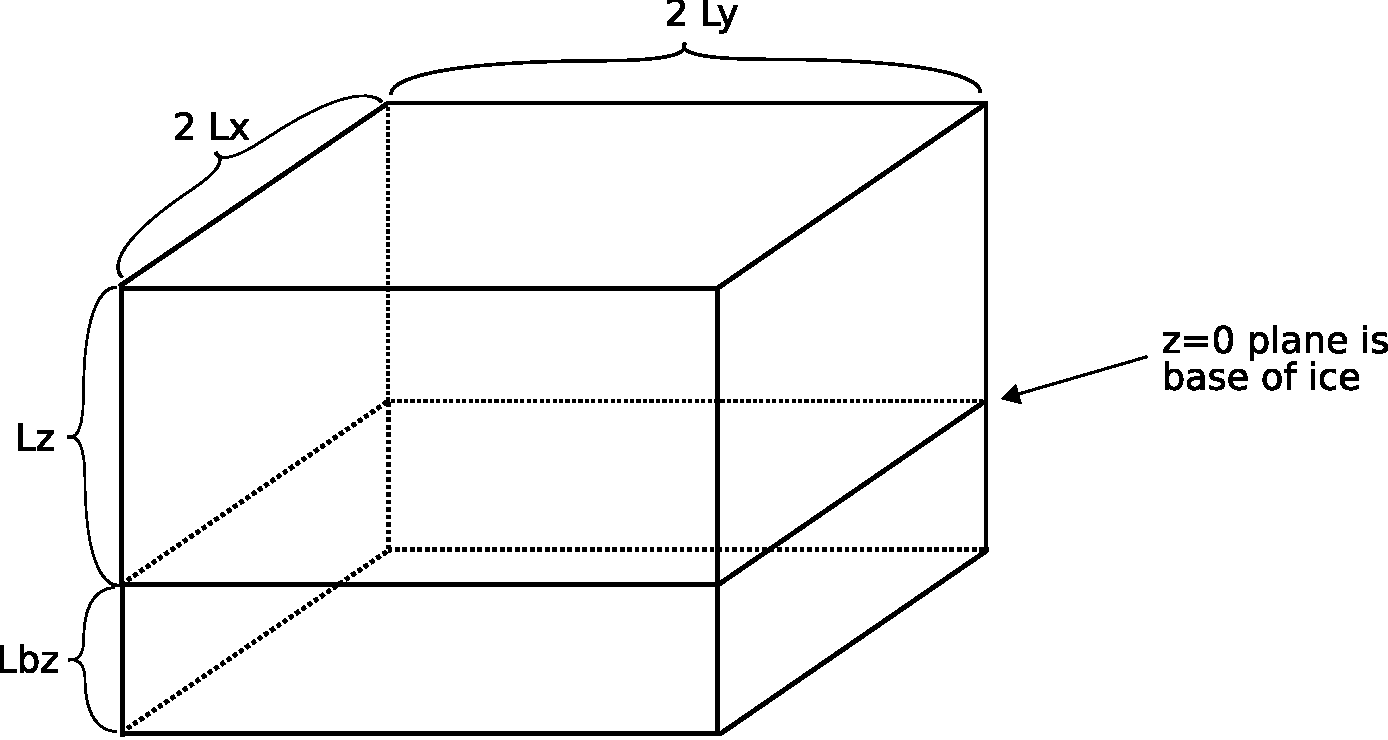
\includegraphics[width=4.0in,keepaspectratio=true]{rectilinearbox}
\caption{PISM's computational box.}
\label{fig:rectilinearbox}
\end{figure}


\subsection{Grid}
\label{subsect:grid}
The PISM grid\index{PISM!grid} covering the computational box is equally spaced in horizontal ($x$ and $y$) directions.  Vertical spacing is quadratic by default (see below) but optionally a different spacing scheme can be chosen.  (Choose with options \intextoption{z\und spacing} and \intextoption{zb\und spacing}.)

The grid is described by four numbers, namely the number of grid points \verb|Mx| in the $x$ direction, the number \verb|My| in the $y$ direction, the number \verb|Mz| in the $z$ direction within the ice, and the number \verb|Mbz| in the $z$ direction within the bedrock thermal layer.  These are specified by options \intextoption{Mx}, \intextoption{My}, \intextoption{Mz}, and \intextoption{Mbz}, respectively, as in Appendix \ref{sect:options}.  The defaults are 61, 61, 31, and 1, respectively.

Note that \verb|Mx|, \verb|My|, \verb|Mz|, and \verb|Mbz| all indicate the number of grid \emph{points}.  The number of grid \emph{spaces} are one less, thus 60, 60, 30, and 0 in the default case.  The lowest grid point in a column of ice, at $z=0$, coincides with the highest grid point in the bedrock, so \verb|Mbz| must always be at least one.

Default spacing is a quadratic function: the spacing is smaller near the base than near the top. (See the documentation of \verb|IceGrid::compute_ice_vertical_levels()| in PISM's class browser for more info and formulas defining the spacing.)

When a thermal bedrock layer is used, the distance \t{Lbz} is controlled by the \intextoption{Lbz} option.

If one initializes PISM from a saved model state using \intextoption{i} then the input model state controls the parameters \t{Mx}, \t{My}, \t{Mz}, and \t{Mbz}.  For instance, the command

\verb|$  pismr -i foo.nc -y 100|

\noindent should work fine if \verb|foo.nc| was a valid PISM model file.  The command

\verb|$  pismr -i foo.nc -Mz 201 -y 100|

\noindent will give a warning that ``\verb|PISM WARNING: ignoring command-line option '-Mz'|'' because \verb|-i| input files take precedence.

Otherwise, one is allowed to specify the grid when PISM is started.  In particular, the user should specify the grid when using \intextoption{boot\und from} or when initializing a simplified geometry experiment or a verification test, though defaults are generally present in these cases.  See sections \ref{sect:start} and \ref{sect:boot} for examples and explanation.

\subsection{Time}
\label{sec:time}

The following command-line options control PISM time.

\optdef{y}{1000} Number of model years to run.

\opt{ye} Model year at which to end the run.  The default value is the start year  (\verb|-ys| or initialized model time from file) plus the default or given (\verb|-y|) run length.  If both \verb|-ys| and \verb|-ye| are used then the run length is set to the difference.  Using all three of \verb|-ys|, \verb|-y| and \verb|-ys| is not allowed.

\opt{ys} Model year at which to start the run.  Also resets the model time, ignoring any time in the input file.



\subsection{Diagnostic computations}  As a diagnostic example, using the EISMINT II final state computed in section \ref{sect:start}, try\index{pismd}

\verb|pismd -i eisIIA200k.nc -o eisIIA200k_diag.nc|

\noindent The result is a NetCDF file \verb|eisIIA200k_diag.nc| which contains the full three-dimensional velocity field in the scalar NetCDF variables \verb|uvel|, \verb|vvel|, and \verb|wvel|.

The velocity field saved by \verb|pismd| is the one which would be computed at the \emph{next} time step in an evolution run.  That is, if we also run\index{pisms}

\verb|pisms -eisII A -i eisIIA200k.nc -y 0 -o eisIIA200k_plus.nc|

\noindent then the horizontal velocity field computed in this single time step run is the same as that saved in \verb|eisIIA200k_diag.nc|.\footnote{For this example, one can use a NetCDF Operator\index{NCO (NetCDF Operators)!ncdiff} to check that the two saved NetCDF files contain the same vertically-averaged horizontal velocity field; just do \t{ncdiff -v cbar} \dots}

This diagnostic mode is most frequently associated to the modeling of ice shelves and ice streams.  Subsection \ref{sect:ross} describes using \verb|pismd| to model the Ross ice shelf \cite{MacAyealetal}.  Verification tests I and J, section \ref{sect:verif}, are diagnostic calculations using the SSA.

Note that the NetCDF model state saved by PISM at the end of an \emph{evolution} run does not, by default, contain the three-dimensional velocity field.  Instead, it contains just the variables which are needed to restart the run, especially the ice geometry and temperature field.  One can also force PISM to save the full velocity field at the end of a time-stepping run using the option \intextoption{f3d}.  The diagnostic executable \verb|pismd| saves the full three-dimensional velocity field by default.  Either way, saving the full velocity field roughly doubles the size of the saved NetCDF file.



\subsection{Computing ice age} \label{subsect:age} By default, PISM does not compute the age of the ice\index{PISM!modeling the age of the ice} because it does not directly impact ice flow using the default flow laws.   It is very easy to turn on.  Just set \intextoption{age}.

\subsection{Setting up PISM boundary (atmosphere, surface and ocean) models}
\label{sec:boundary-models}

Setting up PISM's boundary models requires selecting one model of each kind and zero or more ``model modifiers''; selected models and modifiers are chained as in Figure~\ref{fig:climate-input-data-flow}. Command-line options \intextoption{atmosphere}, \intextoption{surface} and \intextoption{ocean} take a comma-separated list of keywords as an argument; the first keyword \emph{has} to correspond to a model, the rest can be modifiers. Any of these options can be omitted to use the default atmosphere, surface or ocean model, although using a modifier requires specifying a model.

For example,
\begin{verbatim}
$ pismr -i foo.nc -atmosphere searise_greenland,forcing \
        -dTforcing delta_T.nc -surface pdd
\end{verbatim}%$
chooses a combination of SeaRISE-Greenland atmosphere model (see below),  ice-core derived temperature forcing, a PDD local surface mass balance model, and a default (constant) ocean model.

Each of PISM boundary model types currently has one ``modifier'' available; the corresponding keyword is \texttt{forcing}. Please see below for details.

\begin{enumerate}
\item \textbf{PISM atmosphere models.}
  \begin{itemize}
  \item \emph{SeaRISE-Greenland} (\verb|searise_greenland|, the default)

    This atmosphere model implements a longitude, latitude and elevation dependent near-surface air temperature parameterization and a cosine yearly cycle described in \cite{Faustoetal2009} and uses a constant in time ice-equivalent snow precipitation field (in units of thickness per time, variable \verb|snowprecip|) that is read from an input file.

    The parameterization is controlled by configuration parameters with the \texttt{snow\und temp} prefix.

    In addition to the temperature parameterization it implements the SeaRISE-Greenland formula for paleo-precipitation from present; a 7.3\% change of precipitation rate for every one degree Celsius of temperature change \cite{Huybrechts02}

    Please see \url{http://websrv.cs.umt.edu/isis/index.php/Model_Initialization#Greenland} for details.

    It expects variables \verb|snowprecip|, latitude and longitude to be present in an input file.

 \item \emph{Constant in time} (\verb|constant|)

    This atmosphere model reads the snow precipitation (variable \verb|snowprecip|) and the mean annual near-surface air temperature (variable \verb|temp_ma|) and provides them to a surface model.
  \item \emph{Constant precipitation using a temperature lapse rate} (\verb|temp_lapse_rate|)
    
    This atmosphere model also uses a constant snow precipitation field (\verb|snowprecip|) and requires the mean annual near-surface air temperature (\verb|temp_ma|) to be present in an input file. In addition to this, it dynamically corrects air temperature using a location-independent elevation lapse rate specified using the \intextoption{lapse\und rate} command-line option (in units of degrees Celsius per meter).
 \end{itemize}

  The atmosphere \verb|forcing| modifier implements temperature forcing using scalar offsets and also a mechanism applying precipitation and mean annual temperature anomalies.
  \begin{itemize}
  \item \intextoption{dTforcing} specifies a file containing scalar temperature offsets (variable \verb|delta_T|), 
  \item \intextoption{anomaly\und temp\und ma} specifies a file containing spatially-variable mean annual near-surface air temperature anomalies (variable \verb|temp_ma_anomaly|), and
  \item \intextoption{anomaly\und precip} specifies a file containing spatially-variable ice-equivalent precipitation anomalies (in units of thickness per time, variable \verb|snowprecip_anomaly|).
  \end{itemize}

  Options \intextoption{anomaly\und temp\und ma} and \intextoption{anomaly\und precip} can be used to set up a PISM run using a GCM output, essentially achieving one-way coupling.

  Note that only one air temperature forcing mechanism can be used at any time.

\item \textbf{PISM surface (snow) process models}
  \begin{itemize}
  \item \emph{The ``invisible'' model} (\verb|simple|, the default)

    This is the simplest ``surface model'' available in PISM. Its job is to re-interpret  precipitation as mass flux into the ice and mean annual near-surface air temperature as the temperature of the ice at the ice surface (below firn) (see \cite{Hock05}, for example). This implies that there is no melt as long as the precipitation field  is non-negative.

    However primitive it may be, this model can be useful; modeling Antarctica is one example.
  \item \emph{Constant in time} (\verb|constant|)

    This surface model reads constant in time top surface boundary conditions and provides them to the ice dynamics model (see table \ref{tab:ice-dynamics-bc}). When PISM is used with this model, variables \verb|artm| (ice temperature at the ice surface but below firn) and \verb|acab| (top surface mass flux into the ice) are expected to be present in an input file.

    Note: this surface model \emph{ignores}  the atmosphere model selection made using the \intextoption{atmosphere} option.

  \item \emph{Local mass balance (PDD)} (\verb|pdd|) \index{positive degree day model} \index{PDD (positive degree day model)} \index{PISM!default positive degree day model} 

   The default PDD used by PISM, turned on by option \intextoption{surface pdd}, is based on \cite{CalovGreve05} and EISMINT-Greenland intercomparison (section \ref{sec:eismint-greenland} and \cite{RitzEISMINT}). It also implements latitude- and mean July temperature dependent ice and snow factors using formulas in \cite{Faustoetal2009}.

   Our PDD implementation is meant to be used with an atmosphere model implementing a cosine yearly cycle such as \texttt{searise\und greenland}, but is not restricted to parameterizations like this one. A PDD generally adds ``white noise'' to the seasonal cycle to simulate additional daily variability associated to the vagaries of weather.  This additional random variation is quite significant, as the seasonal cycle may never reach the melting point but that point may be reached with some probability, in the presence of the daily variability, and thus melt may occur.  Concretely, a normally-distributed, mean zero random temperature increment is added to the seasonal cycle.  The standard deviation of the daily variability is controlled by the \texttt{pdd\und std\und dev} configuration parameter, and defaults to 2.53 degrees \cite{Faustoetal2009}. There is no particular assumed spatial correlation of daily variability.

The number of positive degree days is computed as the magnitude of the temperature excursion above $0\!\phantom{|}^\circ \text{C}$ multiplied by the duration (in days) when it is above zero.  In PISM there are actually two methods for computing the number of positive degree days.  The first computes only the expected value, by the method described in \cite{CalovGreve05}.  This is the default when a PDD is chosen (i.e.~option \intextoption{surface pdd}).  The second is a monte carlo simulation of the white noise itself, chosen by adding the option \intextoption{pdd\und rand}.  This monte carlo simulation adds the same daily variation at every point, though the seasonal cycle is (generally) location dependent.  If repeatable randomness is desired use \intextoption{pdd\und rand\und repeatable} instead of \verb|-pdd_rand|.

The number of positive degree days is multiplied by a coefficient (config parameter \texttt{pdd\und factor\und snow}) to compute the amount of snow melted.  Of the melted snow, a fraction (\texttt{pdd\und refreeze}) is kept as ice.  This ice, plus all unmelted snow (already measured as ice-equivalent) is added to the mass balance, unless the number of positive degree days exceeds that required to melt all of the snow.  In this latter case, in which there are excess positive degree days available for melting, the excess is multiplied by a coefficient (\texttt{pdd\und factor\und ice}) to compute how much ice is melted.  In this case actual ablation occurs at that location.

See also configuration parameters with the \texttt{pdd\und fausto} prefix.

 \end{itemize}
\item \textbf{PISM ocean models}
  PISM includes one simple ocean model: \verb|constant|, providing constant (both in time and space) mass flux into the ocean and sea level elevation to PISM's ice flow core. The mass flux is controlled by the\\ \verb|ocean_sub_shelf_heat_flux_into_ice| configuration parameter and the assumption that the mass flux is proportional to heat flux into ice.

  The ocean \texttt{forcing} modifier implements sea level forcing. The command-line option \intextoption{dSLforcing} is used to specify the file containing sea level offsets:
\begin{verbatim}
$ pismr -i in.nc -ocean constant,forcing -dSLforcing delta_SL.nc
\end{verbatim}%$
uses \verb|delta_SL.nc|
\end{enumerate}
  
\subsection{Floatation criterion and mask} \label{subsect:floatmask}  The most basic decision about ice dynamics made internally by PISM is whether to apply the ``floatation criterion'' to determine whether the ice is floating on the ocean or not.  In an evolution run this decision is made at each time step and the result is stored in the \t{mask}.

The possible values of the \t{mask}\index{mask} are given in Table \ref{tab:maskvals}.  The mask does not by itself determine ice dynamics.  For instance, when ice is floating (either value \verb|MASK_FLOATING| or \verb|MASK_FLOATING_OCEAN0|) the usual choice for ice dynamics is SSA, but the user can choose not to apply that model by leaving off the option \verb|-ssa|.

\begin{table}[ht]
\caption{The PISM mask\index{mask}, in combination with user options, determines the dynamical model.}\label{tab:maskvals} 
\small
\begin{tabular}{p{0.25\linewidth}p{0.65\linewidth}}\hline
\textbf{Mask value} & \textbf{Meaning}\\ \hline
1=\verb|MASK_SHEET| & ice is grounded (and only the SIA is always applied) \\
2=\verb|MASK_DRAGGING_SHEET| & ice is grounded (and the SSA is applied if option \verb|-ssa| is given) \\
3=\verb|MASK_FLOATING| & ice is floating (and the SSA is applied if option \verb|-ssa| is given) \\
7=\verb|MASK_FLOATING_AT_TIME_0| & same as \verb|MASK_FLOATING|, but the grid point was ice free ocean at initialization of the model by \verb|-boot_from|; ice with this value will calve off if option \verb|-ocean_kill| is given.\\
\hline\end{tabular}
\normalsize
\end{table}

Assuming the geometry of the ice evolves (which can be turned off by option \intextoption{no\und mass}), and assuming an ocean exists (which can be turned off by option \intextoption{dry}), then at each time step the mask can change.  Ice which becomes floating is marked as \verb|MASK_FLOATING| while ice which becomes grounded is either marked as \verb|MASK_SHEET| or \verb|MASK_DRAGGING_SHEET|.  The decision between \verb|MASK_SHEET| or \verb|MASK_DRAGGING_SHEET| is made by a vote-by-neighbors scheme in the most general case.  When both \intextoption{ssa} and \intextoption{super} are given all grounded ice has \verb|MASK_DRAGGING_SHEET|, however.

\subsection{Plastic till free boundary problem for ice streams; SSA as a sliding law}  \label{subsect:plastic}
WARNING: The models described in this subsection are still under active development, and thus we give only a sketch.

The shallow shelf approximation (SSA)\index{SSA (shallow shelf approximation)} stress balance is used in PISM to describe the sliding of grounded ice and the formation of ice streams \cite{BBssasliding}, as well as being used as the only stress balance for floating ice.  For the SSA with ``plastic'' or ``Coulomb'' till the locations of ice streams is determined as part of a free boundary problem \cite{SchoofStream}.  We believe that this mathematical description of ice streams, by Schoof, should be regarded as the best known ``sliding law'' for the SIA \cite{BBssasliding}.\index{SIA (shallow ice approximation)!sliding law}

Schoof's model \cite{SchoofStream} describes emergent ice streams within a larger ice sheet and ice shelf system.  It explains the existence of ice streams by a combination of the plastic failure of the till and the SSA approximation of the balance of momentum.  

In PISM the user gives the options \verb|-ssa -plastic -super| to turn on the use of the plastic till SSA as a sliding law.  All grounded points are immediately marked as SSA (i.e.~as \verb|DRAGGING|).  At these points a yield stress is computed from the amount of stored basal water and from a (generally) spatially-varying till strength, \verb|tillphi| in an input or output file.  The amount of stored basal water is thermodynamically determined.

\begin{table}[ht]
\caption{Using the SSA stress balance in PISM.}\label{tab:ssausage} 
\small
\begin{tabular}{p{0.25\linewidth}p{0.65\linewidth}}\hline
\textbf{Option combination} & \textbf{Meaning}\\ \hline
\intextoption{ssa} & Floating ice uses SSA, and at all points marked \t{DRAGGING}. Basal resistance for grounded ice is plastic (see \intextoption{pseudo\und plastic} to control parameters) but uses fixed field \t{tauc} with no update. \\
\t{-ssa} \intextoption{plastic} & As above, but all grounded points are forced to be \t{DRAGGING} and \t{tauc} is updated at each time step using stored map \t{tillphi} and evolving basal melt water effective thickness \t{bwat}. \\
\t{-ssa -plastic} \intextoption{super} & The recommended default sliding law.  Combines SSA-computed velocity, using plastic till, with SIA-computed velocity as in \cite{BBssasliding}. \\
\hline\end{tabular}
\normalsize
\end{table}

The basal resistance is actually determined by a controllable ``pseudo-plastic'' model.  Specifically, stress is a generally a power law function of basal sliding velocity $\mathbf{u}$:
   $$\tau_b = \tau_c \frac{|\mathbf{u}|^{q-1}}{u_{\text{threshold}}^q}\, \mathbf{u}.$$
Here $\tau_c$ corresponds to the variable \verb|tauc| in PISM input and output files, $q$ is the power controlled by \intextoption{pseudo\und plastic\und q}, and the threshold velocity $u_{\text{threshold}}$ is controlled by \intextoption{pseudo\und plastic\und uthreshold}.  The purely plastic case is $q=0$---see \cite{SchoofStream} for precise interpretation---and the linear case is $q=1$, in which case the coefficient of velocity, $\tau_c/u_{\text{threshold}}$, is more commonly called $\beta$ or $\beta^2$ \cite{MacAyeal}.

In our model the till yield stress $\tau_c$ necessarily represents the strength of the aggregate material at the base of an ice sheet, a poorly observed mixture of liquid water, ice, and granular till.  The value of $\tau_c$ is determined by a basal water model:
\begin{equation*}
   \tau_c = (\tan\phi)\,(\rho g H - p_w).
\end{equation*}
\cite[Chapter 8]{Paterson}.  Here $H$ is the ice thickness, $\rho$ the ice density, $g$ the acceleration of gravity, $p_w$ is the modeled pore water pressure, and $\phi$ is the till friction angle \verb|tillphi|.  The difference $(\rho g H - p_w)$ is the modeled value of the effective pressure on the material till.  Option \intextoption{plastic\und pwfrac} controls how $p_w$ is determined from the effective thickness of basal water, the quantity in \verb|bwat|.

The scripts in \t{examples/pst} perform the experiments described in \cite{BBssasliding}, and represent the most thorough test of these mechanisms.

Test I in the verification suite\index{verification tests} uses an exact solution to the Schoof model, that is, the model described by \t{-ssa -plastic}.

In the \t{-ssa -plastic -super} case especially, the determination of basal resistance comes from a stored basal till material property \verb|tillphi|, the till friction angle.  We find that an effective way to determine \verb|tillphi| is to make it a function of bed elevation.  Option \intextoption{topg\und to\und till} does this.

\subsection{Earth deformation models} \label{subsect:beddef} \index{earth deformation} \index{PISM!earth deformation models, using}   Options
\intextoption{bed\und def\und iso} and \intextoption{bed\und def\und lc} turn on bed deformation models.  The former uses the very minimal assumption of instantaneous pointwise (i.e.~independently at each point in the map plan) isostatic adjustment.  

The latter is much more effective.  It is based on papers by Lingle and Clark \cite{LingleClark}\index{Lingle, Craig} \index{Clark, J.} and \cite{BLKfastearth}.  It is essentially instantaneous computationally because of use of the Fast Fourier Transform to solve the relevant differential equation.  Among other practical features, the rate of bed movement (uplift) is stored in the PISM output file and then is used to initialize the next part of the run.  If observed uplift data is available, it can be used along with \intextoption{boot\und from} to initialize the model so that it starts with the given uplift rate.

Example runs to compare these models are
\begin{verbatim}
$ mpiexec -n 4 pisms -eisII A -z_spacing quadratic -y 8000 -o eisIIA_nobd.nc
$ mpiexec -n 4 pisms -eisII A -z_spacing quadratic -bed_def_iso -y 8000 -o eisIIA_bdiso.nc
$ mpiexec -n 4 pisms -eisII A -z_spacing quadratic -bed_def_lc -y 8000 -o eisIIA_bdlc.nc
\end{verbatim}
Compare the \verb|topg|, \verb|usurf|, and \verb|dbdt| variables in the resulting output files.

Test H in section \ref{sect:verif} can be used to reproduce the comparison done in \cite{BLKfastearth}.

%%% Local Variables: 
%%% mode: latex
%%% TeX-master: "manual"
%%% End: 

% LocalWords:  intercomparison PDD


\clearpage\newpage

\section{Making \emph{HARD} Modeling Choices}
\label{sec:hard-choices}

Most uses of an ice sheet model depend on careful modeling choices in situations where there are considerable uncertainties \emph{and} the model results depend strongly on those choices.  There may be, at the present state of knowledge, \emph{no clear default values} that PISM can provide.

The current section collects some modeling choices which have this ``hard'' flavor.  The available PISM options related to these choices are known to be \emph{not} sufficient for all users.  These are modeling choices for which \emph{we know} the user may have to do a great deal more hard work than just choose among PISM runtime options.  Here are real example cases where users have worked hard:
\begin{itemize}
\item User was required to make use of available data in order to choose parameters for existing PISM models.  These parameters will then override PISM defaults:
\begin{center} % our UAF current situation with Greenland
\fbox{ \begin{minipage}[t]{5.0in}
\emph{Example}.  Use regional atmosphere model output to identify PDD parameters suitable for modeling surface mass balance on a particular ice sheet.  Then supply these parameters to PISM by a \texttt{-config\_override} file.
\end{minipage} }
\end{center}
\item User was required to write code, including code which modified current PISM internals, either to add additional processes or to ``correct'' PISM default process models; or 
\begin{center} % e.g. harder case is Potsdam marine ice sheet mods
\fbox{ \begin{minipage}[t]{5.0in}
\emph{Example}.  Add a new sub-ice-shelf melt model by modifying C++ code in the \texttt{src/coupler/} directory.
\end{minipage} }
\end{center}
\item User deliberately simplified the model in use, instead of the default which was ``throwing in the kitchen sink''.
\begin{center} % Nick's -hold_tauc choice
\fbox{ \begin{minipage}[t]{5.0in}
\emph{Example}.  Instead of using the PISM default mechanism connecting basal melt rate and basal strength, bypass this mechanism and impose a map of yield stress \texttt{tauc} directly.
\end{minipage} }
\end{center}
\end{itemize}

Obviously there is no actual clear distinction between the ``hard'' choices in this section and the ``easy'' ones in the previous section, but the subsections here cover issues for which the PISM developers have a hard time supplying easy answers!

\subsection{Controlling basal strength}  \label{subsect:basestrength}
\optsection{Basal strength and sliding}

In the \texttt{-ssa_sliding} case of a SIA+SSA hybrid model, the determination of basal resistance comes in part from a stored basal till material property $\phi=$\texttt{tillphi}, the till friction angle \cite{Paterson}.  The actual strength value is a till yield stress $\tau_c$, which necessarily represents the strength of the aggregate material at the base of an ice sheet, a poorly observed mixture of liquid water, ice, and granular till.  The value of $\tau_c$ is determined in part by a basal water model and in part by $\phi$, using a Mohr-Coulomb criterion \cite[Chapter 8]{Paterson}, 
\begin{equation*}
   \tau_c = c_{0} + (\tan\phi)\,(\rho g H - p_w).
\end{equation*}
Here $H$ is the ice thickness, $\rho$ the ice density, $g$ the acceleration of gravity, $p_w$ is the modeled pore water pressure, and $\phi$ is the till friction angle.  The difference $(\rho g H - p_w)$ is the modeled value of the effective pressure on the material till.  Note Schoof \cite{SchoofStream} formula (2.4) uses till cohesion $c_0 = 0$ and that is the default value in PISM.

\begin{table}
  \centering
 \begin{tabular}{lp{0.6\linewidth}}
    \\\toprule
    \textbf{Option} & \textbf{Description}
    \\\midrule
    \txtopt{topg_to_phi}{\emph{list of 4 numbers}} & Compute $\phi$ using \eqref{eq:1} and \eqref{eq:2}.\\
    \intextoption{pseudo_plastic} & enables the pseudo-plastic till model \\
    \txtopt{plastic_pwfrac}{\emph{pure number}} & Set what fraction of overburden pressure is assumed as the till pore water pressure.  Only relevant at basal points where there is a positive amount of basal water.\\
    \intextoption{plastic_c0} & Set the value of the till cohesion ($c_{0}$) in the plastic till model.  The value is a pressure, given in kPa.\\
    \txtopt{plastic_reg}{(m/a)} & Set the value of $\eps$ regularization of plastic till; this is the second ``$\eps$'' in formula (4.1) in \cite{SchoofStream}. The default is $0.01$.\\
    \txtopt{plastic_phi}{(degrees)} & Use a constant till friction angle. The default is $30^{\circ}$.\\
    \intextoption{pseudo_plastic_q} & Set the exponent $q$.\\
    \txtopt{pseudo_plastic_uthreshold}{(m/a)} & Set $u_{\text{threshold}}$. The default is $100$ m/a.\\
    \intextoption{hold_tauc} &   Keep the current values of the till yield stress $\tau_c$.  That is, do not update them by the default model using the stored basal melt water.  Only effective if \texttt{-ssa_sliding} is also set.
   \\\bottomrule
  \end{tabular}
\caption{Basal strength command-line options}
\label{tab:basal-strength}
\end{table}

Option \texttt{-plastic_pwfrac} determines $\alpha$, the quantity controlling how $p_w$ is determined from the effective thickness of basal water, the quantity $w=\mathtt{bwat}$; see the next subsection.  The formula is $p_w = \alpha\, w \rho g H$.  See \cite{BKAJS}.

We find that an effective, though heuristic, way to determine \texttt{tillphi} is to make it a function of bed elevation \cite{BKAJS}.  This heuristic is motivated by hypothesis that basal material with a marine history should be weak \cite{HuybrechtsdeWolde}.

Thus PISM has a mechanism setting $\phi$=\texttt{tillphi} to a \emph{piecewise-linear} function of bed elevation.  Given 4 parameters: $\phi_{\mathrm{min}}$, $\phi_{\mathrm{max}}$, $b_{\mathrm{min}}$, $b_{\mathrm{max}}$, where $b$ stands for the bed elevation, let 
\begin{equation}
  M = (\phi_{\text{max}} - \phi_{\text{min}}) / (b_{\text{max}} - b_{\text{min}})\label{eq:1}
\end{equation}
be the slope of the nontrivial part.  Then
\begin{equation}
  \phi(x,y) = \begin{cases}
    \phi_{\text{min}}, & b(x,y) \le b_{\text{min}}, \\
    \phi_{\text{min}} + (b(x,y) - b_{\text{min}}) \,M,
    &  b_{\text{min}} < b(x,y) < b_{\text{max}}, \\
    \phi_{\text{max}}, & b_{\text{max}} \le b(x,y). \end{cases}\label{eq:2}
\end{equation}

Actually the ``yield stress'' $\tau_c$ can be part of a power law model.  In fact, the basal resistance is normally determined by a user-configurable ``pseudo-plastic'' power law.  Specifically, stress is generally a power law function of basal sliding velocity $\mathbf{u}$:
   $$\tau_b = \tau_c \frac{|\mathbf{u}|^{q-1}}{u_{\text{threshold}}^q}\, \mathbf{u}.$$
Here $\tau_c$ corresponds to the variable \texttt{tauc} in PISM input and output files, $q$ is the power controlled by \texttt{-pseudo_plastic_q}, and the threshold velocity $u_{\text{threshold}}$ is controlled by \texttt{-pseudo_plastic_uthreshold}.  The purely plastic case is $q=0$---see \cite{SchoofStream} for precise interpretation---and the linear case is $q=1$, in which case the coefficient of velocity, $\tau_c/u_{\text{threshold}}$, is more commonly called $\beta$ or $\beta^2$ \cite{MacAyeal}.

\begin{quote}
  \textbf{WARNING!} Options \texttt{-pseudo_plastic_q} and \texttt{-pseudo_plastic_uthreshold} have no effect if \texttt{-preudo_plastic} is not set.
\end{quote}


See \emph{PISM Source Code browser}, source files in \texttt{src/base/basal_resistance}, and \cite{BBssasliding,BKAJS} for more details.

The major example of \texttt{-ssa_sliding} usage is in the first section of this manual.  A made-up example, in which sliding happens in the ``trough'', is
\begin{verbatim}
pisms -eisII I -ssa_sliding -Mx 91 -My 91 -Mz 51 \
      -topg_to_phi 5.0,15.0,0.0,1000.0 -y 12000
\end{verbatim}

A final note on basal sliding is in order.  There can be sliding in the SIA stress balance model (paradigm) itself, where the velocity of sliding is a direct function of the driving stress.  Such a SIA sliding mechanism appears in ISMIP-HEINO \cite{Calovetal2009HEINOfinal} and many other SIA-based modeling efforts in the literature.  \emph{This kind of sliding is not recommended, as it does not make sense to regard the driving stress as the local generator of flow if the bed is not holding all of that stress.}  Within PISM there is an implementation of SIA-based sliding for the verification test E, see \texttt{SIA_Sliding.cc}.  PISM does \emph{not} support this sliding mode in other contexts.


\subsection{Subglacial hydrology}  \label{subsect:subhydro}
\optsection{Subglacial hydrology}

Currently, only the most minimal possible hydrology model is implemented in PISM.  By default, the energy conservation calculation generates basal melt and that water is stored locally in the ``till'' under the ice sheet.  The output variable \texttt{bwat} is the effective thickness of this layer of liquid water.  This layer of water relates to the basal boundary condition of the conservation of energy scheme, and it is involved in computing basal water pressure and thus the till yield stress; see the previous subsection.

The minimal model which is on by default is that water is added by basal melt rate, subtracted by refreeze onto the base of the ice, and it decays away in the absence of other inputs according to the configuration parameter \texttt{bwat_decay_rate}.  The amount is bounded above by the configuration constant \texttt{bwat_max}, an effective thickness.  Water above that level is lost in an unmodeled manner.

There is also the option of horizontal diffusion of stored basal water in the field \texttt{bwat}.  This mechanism is normally off, but it is turned on by the option \intextoption{diffuse_bwat}.  The configuration parameters \texttt{bwat_diffusion_distance} and \texttt{bwat_diffusion_time} control the diffusivity.  See equation (11) in \cite{BBssasliding}.

% undocumented options/config. parameters
% base/iMoptions.cc:  "thk_eff" : "thk_eff_basal_water_pressure"
% base/iMoptions.cc:  "thk_eff_H_high" : "thk_eff_H_high"
% base/iMoptions.cc:  "thk_eff_H_low" : "thk_eff_H_low"
% base/iMoptions.cc:  "thk_eff_reduced" : "thk_eff_reduced"
% base/iMoptions.cc:  "bmr_enhance" : "bmr_enhance_basal_water_pressure"
% base/iMoptions.cc:  "bmr_enhance_scale" : "bmr_enhance_scale"


%%% Local Variables: 
%%% mode: latex
%%% TeX-master: "manual"
%%% End: 

% LocalWords:  PDD pdd html PISM PISM's paleo


\clearpage\newpage

\section{Practical usage}
\label{sec:practical-usage}

\subsection{Input and output}
\label{sec:input-output}
\optsection{Input and output}
\optseealso{Bootstrapping}
\optseealso{Regridding}

PISM is a program that reads NetCDF files and then outputs NetCDF files.  Table \ref{tab:input-output-options} summarizes command-line options controlling the most basic ways to input and output NetCDF files when starting and ending PISM runs.

\begin{table}[ht]
  \centering
 \begin{tabular}{lp{0.6\linewidth}}
    \toprule
    \textbf{Option} & \textbf{Description} \\
    \midrule
    \fileopt{i} & Chooses a PISM output file (NetCDF format) to initialize or restart from.  See section \ref{sec:initboot}. \\
    \fileopt{boot_file} & Chooses a NetCDF file to bootstrap from, using heuristics to ``fill in'' missing fields.  See section \ref{sec:initboot}. \\
    \intextoption{dontreadSSAvels} & Turns off reading the \texttt{ubar_ssa} and \texttt{vbar_ssa} velocities saved by a previous run using the \texttt{ssa} or \texttt{ssa+sia} stress balance (see section \ref{subsect:stressbalance}). \\ \midrule
    \fileopt{o} & Chooses the output file name.  Default name is \texttt{unnamed.nc}.\\
    \txtopt{o_size}{$\left<\text{size}\right>$} & Chooses the ``size'' of the output file to produce.  Possible sizes are \texttt{none} (\emph{no} output file at all), \texttt{small} (only variables necessary to restart PISM), \texttt{medium} (the default, includes a few diagnostic quantities) and \texttt{big} (writes all the variables mentioned in Tables~\ref{tab:three-d-diagnostics},~\ref{tab:three-d-diagnostics-vector},~\ref{tab:two-d-diagnostics-1},~\ref{tab:two-d-diagnostics-2},~\ref{tab:two-d-diagnostics-3},~and~\ref{tab:two-d-diagnostics-vector}).  Configuration variables \texttt{output_medium} and \texttt{output_big} list the written variables for those sizes. \\
    \bottomrule
 \end{tabular}
\caption{Basic NetCDF input and output options}
\label{tab:input-output-options}
\end{table}

Table \ref{tab:stdout} lists the controls on what is printed to the standard output.  Note the \texttt{-help} and \texttt{-usage} options for getting help at the command line.

\begin{table}[ht]
  \centering
 \begin{tabular}{lp{0.7\linewidth}}
    \toprule
    \textbf{Option} & \textbf{Description} \\
    \midrule 
    \intextoption{help} &  Brief descriptions of the many PISM and PETSc options.  The run occurs as usual according to the other options.  (The option documentation does not get listed if the run didn't get started properly.)  Use with a pipe into \texttt{grep} to get usefully-filtered information on options, for example ``\texttt{pisms -help | grep cold}''. \\
    \intextoption{info} & Gives information about PETSc operations during the run. \\
   \intextoption{list_diagnostics}  & Prints a list of all available diagnostic outputs (time series and spatial) for the run with the given options.  Stops run after printing the list. \\
   \intextoption{log_summary}  & At the end of the run gives a performance summary and also a synopsis of the PETSc configuration in use.\\
   \intextoption{options_left} & At the end of the run shows an options table which will indicate if
   a user option was not read or was misspelled.\\
   \intextoption{usage} &   Short summary of PISM executable usage, without listing all the options, and without doing the run.\\
   \midrule
   \intextoption{verbose} & Increased verbosity of standard output.  Usually given with an integer level; 0,1,2,3,4,5 are allowed.  If given without argument then sets level 3, while ``\texttt{-verbose 2}'' is the default (i.e.~equivalent to no option).  At the extremes, \texttt{-verbose 0} produces no stdout at all, \texttt{-verbose 1} prints only warnings and a few high priority messages, and \texttt{-verbose 5} spews a lot of usually-undesirable stuff.  \texttt{-verbose 3} output regarding initialization may be useful.  \\
   \midrule
   \intextoption{version} &   Show version numbers of PETSc and PISM.\\
   \bottomrule
  \end{tabular}
\caption{Options controlling PISM's standard output}
\label{tab:stdout}
\end{table}

The following sections describe more input and output options, especially related to saving quantities during a run, or adding to the ``diagnostic'' outputs of PISM.

\clearpage

\subsubsection{PISM file I/O performance}
\label{sec:pism-io-performance}

When working with fine grids\footnote{For example, resolutions of 2km and higher on the whole-Greenland scale.}, the time PISM spends writing output files, spatially-varying diagnostic files, or backup files can become significant.

It turns out that it is a lot faster to read and write files using the \texttt{t,x,y,z} storage order, as opposed to the more convenient (e.g.~for NetCDF tools) \texttt{t,z,y,x} order.  The reason is that PISM uses the \texttt{x,y,z} order internally,\footnote{This is not likely to change.} and therefore writing an array in a different order is an inherently-expensive operation.

You can, however, choose any one of the three supported output orders using the \intextoption{o_order} option with one of \texttt{xyz}, \texttt{yxz}, and \texttt{zyx} as the argument.

To transpose dimensions in an existing file, use the \texttt{ncpdq} (``permute dimensions quickly'') tool from the NCO (\emph{NetCDF Operators}) suite.  For example, run
\begin{verbatim}
$ ncpdq -a t,z,zb,y,x bad.nc good.nc
\end{verbatim}
%$ - match dollar signs to make emacs happy
to turn \texttt{bad.nc} (with any inconvenient storage order) into \texttt{good.nc} using the \texttt{t,z,y,x} order.

PISM also supports NetCDF-4 parallel I/O, which gives better performance in
high-resolution runs and avoids NetCDF-3 file format limitations. (In a
NetCDF-3 file a variable record cannot exceed 4 gigabytes.) Build PISM with
parallel NetCDF-4 and use \intextoption{o_format} \texttt{netcdf4_parallel} to
enable this code.

In addition to \texttt{-o_format netcdf4_parallel} and \texttt{netcdf3}
(default) modes, PISM can be built with PnetCDF for best I/O performance. The
option \texttt{-o_format pnetcdf} turns ``on'' PnetCDF I/O code. (PnetCDF seems
to be somewhat fragile, though, so use at your own risk.)


\subsection{Saving time series of scalar diagnostic quantities}
\index{time-series}\index{PISM!saving time-series}
\label{sec:saving-time-series}
\optsection{Saving scalar time-series}

 It is also possible to save time-series of certain scalar diagnostic quantities using a combination of the options \texttt{-ts_file}, \texttt{-ts_times}, and \texttt{-ts_vars}.  For example,
\begin{verbatim}
$ pismr -i foo.nc -y 1e4 -o output.nc -ts_file time-series.nc \
        -ts_times 0:1:1e4 -ts_vars ivol,iareag
\end{verbatim}
%$ - match dollar signs to make emacs happy
will run for 10000 years, saving total ice volume and grounded ice area to \texttt{time-series.nc} \emph{yearly}. See tables \ref{tab:time-series-opts} for the list of options and \ref{tab:time-series-1}~and~\ref{tab:time-series-2} for the full list of supported time-series.

Note that, similarly to the snapshot-saving code (section \ref{sec:snapshots}), this mechanism does not affect adaptive time-stepping.  Here, however, PISM will save exactly the number of time-series records requested, \emph{linearly interpolated onto requested times}.

Omitting the \texttt{-ts_vars} option makes PISM save \emph{all} available
variables, as listed in tables
\ref{tab:time-series-1}~and~\ref{tab:time-series-2}.  Because scalar
time-series take minimal storage space, compared to spatially-varying data,
this is usually a reasonable choice. Run PISM with the
\intextoption{list_diagnostics} option to see the list of all available time-series.

If the file \texttt{foo.nc}, specified by \texttt{-ts_file foo.nc}, already exists then by default the existing file will be moved to \texttt{foo.nc~} and the new time series will go into \texttt{foo.nc}.  To append the time series onto the end of the existing file, use option \texttt{-ts_append}.

PISM buffers time-series data and writes it at the end of the run, once 10000
values are stored, or when an \texttt{-extra_file} is saved, whichever comes first. Sending an \texttt{USR1} (or
\texttt{USR2}) signal to a PISM process flushes these buffers, making it
possible to monitor the run. (See section \ref{subsect:signal} for more about
PISM's signal handling.)

\begin{table}[ht]
 \centering
 \begin{tabular}{p{0.35\linewidth}p{0.55\linewidth}}\toprule
    \textbf{Option} & \textbf{Description} \\
    \midrule
    \fileopt{ts_file} & Specifies the file to save to.\\
    \timeopt{ts_times} & Specifies times to save at as a MATLAB-style range $a:\Delta t:b$, a comma-separated list, or a keyword (\texttt{hourly}, \texttt{daily}, \texttt{monthly}, \texttt{yearly}). See section \ref{sec:saving-spat-vari}. \\
    \listopt{ts_vars} & Comma-separated list of variables, see
    tables~\ref{tab:time-series-1}~and~\ref{tab:time-series-2}. Omitting this
    option is equivalent to listing the \emph{all} variables.\\
    \intextoption{ts_append} & Append time series to file if it already exists.  No effect if file does not yet exist. \\
    \bottomrule
  \end{tabular}
\caption{Command-line options controlling saving scalar time-series}
\label{tab:time-series-opts}
\end{table}

Besides the above information on usage, here are comments on the physical significance of several scalar diagnostics which appear in tables \ref{tab:time-series-1}~and~\ref{tab:time-series-2}:\index{PISM!physical meaning of scalar diagnostics}
\begin{itemize}
  \item For each variable named \dots\texttt{_flux}, positive values mean ice sheet mass gain.
  \item The \texttt{sub_shelf_ice_flux} may be non-zero even if \texttt{iareaf} (floating ice area) is zero. This is due to the fact that during time-stepping fluxes are computed before calving is applied, and the ice area is computed \emph{after} calving. Hence ice that is calved off experiences top-surface and basal fluxes, but does not contribute to the reported area. This is a small error that approaches zero as the grid is refined. In this case \texttt{sub_shelf_ice_flux} should be added to the calving flux during post-processing.
%FIXME \footnote{This will be fixed in a later release of PISM.}
  \item Ice volume and area are computed and then split among floating and grounded portions: \texttt{ivol} $\mapsto$ (\texttt{ivolf}, \texttt{ivolg}) while \texttt{iarea} $\mapsto$ (\texttt{iareaf},\texttt{iareag}).  The volumes have units \textsl{$m^3$} and the areas have units \textsl{$m^2$}.
  \item The thermodynamic state of the ice sheet can be assessed, in part, by the amount of cold or temperate (``\texttt{temp}'') ice.  Thus there is another splitting: \texttt{ivol} $\mapsto$ (\texttt{ivolcold}, \texttt{ivoltemp}) and \texttt{iarea} $\mapsto$ (\texttt{iareacold},\texttt{iareatemp}).
  \item If a PISM input file contains the \texttt{proj4} global attribute with a PROJ.4 string defining the projection then PISM computes corrected cell areas
using this information, grid parameters, and the WGS84 reference ellipsoid. This yields areas and volumes with greater accuracy.
  \item The sea-level-relevant ice volume \texttt{slvol} is the total grounded ice volume minus the amount of ice, that, in liquid form, would fill up the regions with bedrock below sea level, if this ice were removed.  That is, \texttt{slvol} is the sea level rise potential of the ice sheet at that time.  The result is reported  in sea-level equivalent, i.e.~meters of sea level rise.
  \item Fields \texttt{max_diffusivity} and \texttt{max_hor_vel} relate to PISM time-stepping.  These quantities appear in per-time-step form in the standard output from PISM (i.e.~at default verbosity).  \texttt{max_diffusivity} determines the length of the mass continuity substeps for the SIA stress balance (sub-)model.  \texttt{max_hor_vel} determines the CFL-type restriction for mass continuity and conservation of energy contributions of the SSA stress balance (i.e.~sliding) velocity.
\end{itemize}

\begin{table}[ht]
  \centering
 \begin{tabular}{p{0.4\linewidth}p{0.1\linewidth}p{0.4\linewidth}}
    \toprule
    \textbf{Name} & \textbf{Units} & \textbf{Description}\\
    \midrule
    \texttt{cumulative_grounded_basal_ice_flux} & \textsl{kg} &  cumulative total grounded basal ice flux \\
    \texttt{cumulative_discharge_flux} & \textsl{kg} &  cumulative discharge (calving etc.) flux \\
    \texttt{cumulative_float_kill_flux} & \textsl{kg} &  cumulative \texttt{-float_kill} flux \\
    \texttt{cumulative_nonneg_rule_flux} & \textsl{kg} &  cumulative \emph{numerical} ice flux resulting from enforcing the $\mathrm{thk} \ge 0$ rule \\
    \texttt{cumulative_ocean_kill_flux} & \textsl{kg} &  cumulative \texttt{-calving ocean_kill} flux \\
    \texttt{cumulative_sub_shelf_ice_flux} & \textsl{kg} &  cumulative total sub-shelf ice flux \\
    \texttt{cumulative_surface_ice_flux} & \textsl{kg} &  cumulative total over ice domain of top surface ice mass flux \\
    \texttt{dimassdt} & \textsl{kg  / s} &  total ice mass rate of change \\
    \texttt{discharge_flux} & \textsl{kg  / s} &  discharge (calving and icebergs) flux \\
    \texttt{divoldt} & \textsl{$m^{3}$  / s} &  total ice volume rate of change \\
    \texttt{dt} & \textsl{second} &  mass continuity time step \\
    \texttt{float_kill_flux} & \textsl{kg  / s} &  \texttt{-float_kill} flux \\
    \texttt{grounded_basal_ice_flux} & \textsl{kg  / s} &  total, over grounded ice, of basal ice flux \\
    \texttt{iarea} & \textsl{$m^{2}$} &  total ice area \\
    \texttt{iareacold} & \textsl{$m^{2}$} &  ice-covered area where basal ice is cold \\
    \texttt{iareaf} & \textsl{$m^{2}$} &  total floating ice area \\
    \texttt{iareag} & \textsl{$m^{2}$} &  total grounded ice area \\
    \texttt{iareatemp} & \textsl{$m^{2}$} &  ice-covered area where basal ice is temperate \\
    \texttt{ienthalpy} & \textsl{J} &  total ice enthalpy \\
    \multicolumn{3}{c}{Continued in Table \ref{tab:time-series-2}}\\
    \bottomrule
  \end{tabular}
\caption{Scalar time-series supported by PISM, part 1}
\label{tab:time-series-1}
\end{table}

\begin{table}[ht]
  \centering
 \begin{tabular}{p{0.4\linewidth}p{0.1\linewidth}p{0.4\linewidth}}
    \toprule
    \textbf{Name} & \textbf{Units} & \textbf{Description}\\
    \midrule
    \multicolumn{3}{c}{Continued from Table \ref{tab:time-series-1}}\\
    \texttt{imass} & \textsl{kg} &  total ice mass \\
    \texttt{ivol} & \textsl{$m^{3}$} &  total ice volume \\
    \texttt{ivolcold} & \textsl{$m^{3}$} &  total volume of cold ice \\
    \texttt{ivolf} & \textsl{$m^{3}$} &  total floating ice volume \\
    \texttt{ivolg} & \textsl{$m^{3}$} &  total grounded ice volume \\
    \texttt{ivoltemp} & \textsl{$m^{3}$} &  total volume of temperate ice \\
    \texttt{max_diffusivity} & \textsl{$m^{2}$  / s} &  maximum diffusivity \\
    \texttt{max_hor_vel} & \textsl{m  / s} &  maximum (absolute) component of horizontal ice velocity over the grid \\
    \texttt{nonneg_rule_flux} & \textsl{kg  / s} &  \emph{numerical} ice flux resulting from enforcing the $\mathrm{thk} \ge 0$ rule \\
    \texttt{ocean_kill_flux} & \textsl{kg  / s} &  \texttt{-calving ocean_kill} flux \\
    \texttt{slvol} & \textsl{m} &  total sea-level relevant ice \textbf{in sea-level equivalent} \\
    \texttt{sub_shelf_ice_flux} & \textsl{kg  / s} &  total sub-shelf ice flux \\
    \texttt{surface_ice_flux} & \textsl{kg  / s} &  total over ice domain of top surface ice mass flux \\
    \bottomrule
  \end{tabular}
\caption{Scalar time-series supported by PISM, part 2}
\label{tab:time-series-2}
\end{table}

\clearpage

\subsection{Saving time series of spatially-varying diagnostic quantities}
\label{sec:saving-spat-vari}
\optsection{Saving 2D and 3D time-series}
\index{PISM!saving diagnostic quantities regularly}
\index{PISM!diagnostic quantities}

Sometimes it is useful to have PISM save a handful of diagnostic \emph{maps} at some interval like every 10 years or even every month.  One can use snapshots (section \ref{sec:snapshots}), but doing so can easily fill your hard-drive because snapshots are complete (i.e.~re-startable) model states.  Sometimes you want a \emph{subset} of model variables saved frequently in an output file.

Use options \texttt{-extra_file}, \texttt{-extra_times}, and \texttt{-extra_vars} for this.  For example,
\begin{verbatim}
$ pismr -i foo.nc -y 10000 -o output.nc -extra_file extras.nc \
        -extra_times 0:10:1e4 -extra_vars velsurf_mag,velbase_mag
\end{verbatim}
%$ - match dollar signs to make emacs happy
will run for 10000 years, saving the magnitude of horizontal velocities at the ice surface and at the base of ice every 10 years.  Times are specified using a comma-separated list or a MATLAB-style range.  See Table \ref{tab:extras} for all the options controlling this feature.  Tables~\ref{tab:three-d-diagnostics},~\ref{tab:three-d-diagnostics-vector},~\ref{tab:two-d-diagnostics-1},~\ref{tab:two-d-diagnostics-2},~\ref{tab:two-d-diagnostics-3},~and~\ref{tab:two-d-diagnostics-vector} list all the variable choices.

Note that options \intextoption{extra_times},
\intextoption{save_times}, \intextoption{ts_times} take \emph{dates}
if a non-trivial calendar is selected. For example,
\begin{verbatim}
pismr ... -extra_times 10       # every 10 years
pismr ... -extra_times 2days    # every 2 days
pismr ... -calendar gregorian -extra_times 1-1-1:daily:11-1-1 # daily for 10 years
pismr ... -calendar gregorian -extra_times daily -ys 1-1-1 -ye 11-1-1
pismr ... -calendar gregorian -extra_times 2hours -ys 1-1-1 -ye 1-2-1
\end{verbatim}

The step in the range specification can have the form \texttt{Nunit},
for example \texttt{5days}. Units based on ``months'' and ``years''
are not supported if a non-trivial calendar is selected.

In addition to specifying a constant step in \texttt{-extra_times a:step:b} one can save every hour, day, month, or every year by using \texttt{hourly}, \texttt{daily}, \texttt{monthly} or \texttt{yearly} instead of a number; for example
\begin{verbatim}
$ pismr -i foo.nc -y 100 -o output.nc -extra_file extras.nc \
        -extra_times 0:monthly:100 -extra_vars dHdt
\end{verbatim}
%$ - match dollar signs to make emacs happy
will save the rate of change of the ice thickness every month for 100
years. With \texttt{-calendar none} (the default), ``monthly'' means
``every $\frac 1 {12}$ of the year'', and ``yearly'' is ``every
$3.14\dots\times10^7$ seconds, otherwise PISM uses month lengths
computed using the selected calendar.

It is frequently desirable to save diagnostic quantities at regular intervals for the whole duration of the run; options \intextoption{extra_times}, \intextoption{ts_times}, and \intextoption{save_times} provide a shortcut. For example, use \texttt{-extra_times yearly} to save at the end of every year.

This is especially useful when using a climate forcing file to set run duration:
\begin{verbatim}
$ pismr -i foo.nc -surface given -surface_given_file climate.nc \
        -calendar gregorian -time_file climate.nc \
        -extra_times monthly -extra_file ex.nc -extra_vars thk
\end{verbatim}
%$ - match dollar signs to make emacs happy
will save ice thickness at the end of every month while running PISM for the duration of climate forcing data in \texttt{climate.nc}.

Times given using \texttt{-extra_times} describe the reporting intervals by giving the endpoints of these reporting intervals.  The save itself occurs at the end of each interval.  This implies, for example, that \texttt{0:1:10} will produce 10 records at times 1,\dots,10 and \emph{not} 11 records.

If the file \texttt{foo.nc}, specified by \texttt{-extra_file foo.nc}, already exists then by default the existing file will be moved to \texttt{foo.nc\~} and the new time series will go into \texttt{foo.nc}.  To append the time series onto the end of the existing file, use option \texttt{-extra_append}.

The list of available diagnostic quantities depends on the model setup. For
example, a run with only one vertical grid level in the bedrock thermal layer
will not be able to save \texttt{litho_temp}, an SIA-only run does not use a
basal yield stress model and so will not provide \texttt{tauc}, etc. To see
which quantities are available in a particular setup, use the
\intextoption{list_diagnostics} option, which prints the list of diagnostics
and stops.

The \texttt{-extra_file} mechanism modifies PISM's adaptive time-stepping scheme so as to step to, and save at,
\emph{exactly} the times requested.  By contrast, as noted in subsection \ref{sec:saving-time-series}, the \texttt{-ts_file} mechanism does not alter PISM's time-steps and instead uses linear interpolation to save at the requested times in between PISM's actual time-steps.

\begin{table}[ht]
 \centering
 \begin{tabular}{p{0.35\linewidth}p{0.55\linewidth}}\toprule
    \textbf{Option} & \textbf{Description}\\
    \midrule
    \fileopt{extra_file} & Specifies the file to save to; should be different from the output \texttt{o} file.\\
    \timeopt{extra_times} & Specifies times to save at either as a MATLAB-style range $a:\Delta t:b$ or a comma-separated list.\\
    \listopt{extra_vars} & Comma-separated list of variables, see
    tables~\ref{tab:three-d-diagnostics},~\ref{tab:two-d-diagnostics-1},~\ref{tab:two-d-diagnostics-2},~and~\ref{tab:two-d-diagnostics-3} \\
    \intextoption{extra_split} & Save to separate files, similar to \texttt{-save_split}\\
    \intextoption{extra_append} & Append variables to file if it already exists.  No effect if file does not yet exist, and no effect if \intextoption{extra_split} is set. \\
    \bottomrule
  \end{tabular}
\caption{Command-line options controlling extra diagnostic output}
\label{tab:extras}
\end{table}

\begin{table}[ht]
  \centering
  \begin{tabular}{p{0.15\linewidth}p{0.15\linewidth}p{0.6\linewidth}}
    \toprule
    \textbf{Name} & \textbf{Units} & \textbf{Description} \\
    \midrule
    \texttt{age} & \textsl{s} & age of ice \\
    \texttt{enthalpy} & \textsl{J $\mathrm{kg}^{-1}$} & ice enthalpy (includes sensible heat, latent heat, pressure) \\
    \texttt{temp} & \textsl{K} & ice temperature \\
    \texttt{cts} & \textsl{none} &  $\mathrm{cts} = E/E_s(p)$, so cold-temperate transition surface is at $\mathrm{cts} = 1$ \\
    \texttt{liqfrac} & \textsl{1} &  liquid water fraction in ice (between $0$ and $1$) \\
    \texttt{litho_temp} & \textsl{K} & lithosphere (bedrock) temperature, in \texttt{PISMBedThermalUnit} \\
    \texttt{temp} & \textsl{K} &  ice temperature \\
    \texttt{temp_pa} & \textsl{degrees Celsius} &  pressure-adjusted ice temperature (degrees above pressure-melting point) \\
    \bottomrule
  \end{tabular}
\caption{Scalar 3D diagnostic quantities}
\label{tab:three-d-diagnostics}
\end{table}

\begin{table}[ht]
  \centering
  \begin{tabular}{p{0.15\linewidth}p{0.15\linewidth}p{0.6\linewidth}}
    \toprule
    \textbf{Name} & \textbf{Units} & \textbf{Description} \\
    \midrule
    \texttt{uvel} & \textsl{m / year} &  horizontal velocity of ice in the X direction \\
    \texttt{vvel} & \textsl{m / year} &  horizontal velocity of ice in the Y direction \\
    \texttt{wvel} & \textsl{m / year} &  vertical velocity of ice, relative to geoid \\
    \texttt{wvel_rel} & \textsl{m / year} &  vertical velocity of ice, relative to base of ice directly below \\
    \bottomrule
  \end{tabular}
\caption{Vector 3D diagnostic quantities}
\label{tab:three-d-diagnostics-vector}
\end{table}

\begin{table}[ht]
  \centering
  \begin{tabular}{p{0.15\linewidth}p{0.15\linewidth}p{0.6\linewidth}}
    \toprule
    \textbf{Name} & \textbf{Units} & \textbf{Description} \\
    \midrule
    \texttt{bedtoptemp} & \textsl{K} & temperature of top of bedrock thermal layer \\
    \texttt{bfrict} & \textsl{W  / $m^2$} &  basal frictional heating \\
    \texttt{bheatflx} & \textsl{W  / $m^2$} & upward geothermal flux at bedrock surface \\
    \texttt{bmelt} & \textsl{m / year} & ice basal melt rate in ice thickness per time \\
    \texttt{bwat} & \textsl{m} & effective thickness of subglacial melt water \\
    \texttt{bwp} & \textsl{Pa} & subglacial (pore) water pressure \\
    \texttt{cell_area} & \textsl{$m^{2}$} & cell areas \\
    \texttt{climatic_mass_balance} & \textsl{m / year} & ice-equivalent surface mass balance (accumulation/ablation) rate \\
    \texttt{dHdt} & \textsl{m / year} &  ice thickness rate of change \\
    \texttt{dbdt} & \textsl{m / year} & bedrock uplift rate \\
    \texttt{deviatoric_stresses} & \textsl{Pa} & 2D deviatoric stresses (this saves 3 fields: in the $X$ direction, in the $Y$ direction, and the shear stress) \\
    \texttt{diffusivity} & \textsl{$m^{2}$  / s} &  diffusivity of SIA mass continuity equation \\
    \texttt{enthalpybase} & \textsl{J  / kg} &  ice enthalpy at the base of ice \\
    \texttt{enthalpysurf} & \textsl{J  / kg} &  ice enthalpy at 1m below the ice surface \\
    \texttt{flux_divergence} & \textsl{m / year} &  flux divergence \\
    \texttt{flux_mag} & \textsl{$m^{2}$ / year} &  magnitude of vertically-integrated horizontal flux of ice \\
    \texttt{hardav} & $Pa\, s^{1/n}$ &  vertical average of ice hardness \\
    \texttt{ice_surface_temp} & \textsl{K} & annual average ice surface temperature, below firn processes \\
    \texttt{lat} & \textsl{degrees north} & latitude \\
    \texttt{lon} & \textsl{degrees east} & longitude \\
    \texttt{velbar_mag} & \textsl{m / year} &  magnitude of vertically-integrated horizontal velocity of ice \\
    \texttt{velbase_mag} & \textsl{m / year} &  magnitude of horizontal velocity of ice at base of ice \\
    \texttt{velsurf_mag} & \textsl{m / year} &  magnitude of horizontal velocity of ice at ice surface \\
   \multicolumn{3}{c}{Continued in Table \ref{tab:two-d-diagnostics-2}}\\
  \bottomrule
  \end{tabular}
  \caption{Scalar 2D diagnostic quantities, part 1}
  \label{tab:two-d-diagnostics-1}
\end{table}

\begin{table}[ht]
  \centering
  \begin{tabular}{p{0.15\linewidth}p{0.15\linewidth}p{0.6\linewidth}}
    \toprule
    \textbf{Name} & \textbf{Units} & \textbf{Description} \\
    \midrule
    \multicolumn{3}{c}{Continued from Table \ref{tab:two-d-diagnostics-1}}\\
    \texttt{mask} & \textsl{none} & grounded/dragging/floating integer mask \\
    \texttt{proc_ice_area} & \textsl{none} &  number of cells containing ice in a processor's domain \\
    \texttt{rank} & \textsl{none} &  processor rank \\
    \texttt{schoofs_theta} & \textsl{1} &  multiplier $\theta$ in \cite{Schoofbasaltopg2003} \\
    \texttt{shelfbmassflux} & \textsl{m / year} & ice mass flux from ice shelf base (positive flux is loss from ice shelf) \\
    \texttt{shelfbtemp} & \textsl{Kelvin} & absolute temperature at ice shelf base \\
    \texttt{strain_rates} & \textsl{1/s} & eigenvalues of the horizontal, vertically-integrated strain rate tensor \\
    \texttt{taub_mag} & \textsl{Pa} & magnitude of the basal shear stress \\
    \texttt{tauc} & \textsl{Pa} & yield stress for basal till (plastic or pseudo-plastic model) \\
    \texttt{taud_mag} & \textsl{Pa} &  magnitude of the driving stress at the base of ice \\
    \texttt{tempbase} & \textsl{K} &  ice temperature at the base of ice \\
    \texttt{tempicethk_basal} & \textsl{m} &  thickness of the basal layer of temperate ice \\
    \texttt{tempicethk} & \textsl{m} &  temperate ice thickness (total column content) \\
    \texttt{temppabase} & \textsl{Celsius} &  pressure-adjusted ice temperature at the base of ice \\
    \texttt{tempsurf} & \textsl{K} &  ice temperature at 1m below the ice surface \\
    \texttt{thksmooth} & \textsl{m} &  thickness relative to smoothed bed elevation in \cite{Schoofbasaltopg2003} \\
    \texttt{thk} & \textsl{m} & land ice thickness \\
    \texttt{tillphi} & \textsl{degrees} & friction angle for till under grounded ice sheet \\
    \texttt{topgsmooth} & \textsl{m} &  smoothed bed elevation in \cite{Schoofbasaltopg2003}\\
    \texttt{topg} & \textsl{m} & bedrock surface elevation \\
    \texttt{usurf} & \textsl{m} & ice upper surface elevation \\
   \multicolumn{3}{c}{Continued in Table \ref{tab:two-d-diagnostics-3}}\\
  \bottomrule
  \end{tabular}
  \caption{Scalar 2D diagnostic quantities, part 2}
  \label{tab:two-d-diagnostics-2}
\end{table}

\begin{table}[ht]
  \centering
  \begin{tabular}{p{0.15\linewidth}p{0.15\linewidth}p{0.6\linewidth}}
    \toprule
    \textbf{Name} & \textbf{Units} & \textbf{Description} \\
    \midrule
    \multicolumn{3}{c}{Continued from Table \ref{tab:two-d-diagnostics-2}}\\
    \texttt{floating_basal_flux_cumulative} & \textsl{Gt} & cumulative basal flux into the ice in floating areas \\
    \texttt{grounded_basal_flux_cumulative} & \textsl{Gt} & cumulative basal flux into the ice in grounded areas \\
    \texttt{nonneg_flux_cumulative} & \textsl{Gt} & cumulative numerical flux created by enforcing non-negativity of ice thickness \\
    \texttt{ocean_kill_flux_cumulative} & \textsl{Gt} & cumulative version of \texttt{ocean_kill_flux} \\
    \texttt{ocean_kill_flux} & \textsl{kg / s} & calving flux due to the ``\texttt{-calving ocean_kill}'' mechanism \\
    \bottomrule
  \end{tabular}
  \caption{Scalar 2D diagnostic quantities, part 3}
  \label{tab:two-d-diagnostics-3}
\end{table}

\begin{table}[ht]
  \centering
  \begin{tabular}{p{0.15\linewidth}p{0.15\linewidth}p{0.6\linewidth}}
    \toprule
    \textbf{Name} & \textbf{Units} & \textbf{Description} \\
    \midrule
    \texttt{h_x} & \textsl{none} &  the x-component of the surface gradient, on the staggered grid\\
    \texttt{h_y} & \textsl{none} &  the y-component of the surface gradient, on the staggered grid\\
    \texttt{taub} & \textsl{Pa} & basal shear stress, X and Y components. See also \texttt{taub_mag}. \\
    \texttt{taud} & \textsl{Pa} & driving stress at the base of ice, X and Y components. See also \texttt{taud_mag}. \\
    \texttt{velbar} & \textsl{m / year} &  vertical mean of horizontal ice velocity in the X and Y directions. See also \texttt{velbar_mag}. \\
    \texttt{velbase} & \textsl{m / year} &  horizontal velocity of ice at the base of ice in the X and Y directions. See also \texttt{velbase_mag}. \\
    \texttt{velsurf} & \textsl{m / year} &  horizontal velocity of ice at ice surface in the X and Y directions. See also \texttt{velsurf_mag}.\\
    \texttt{wvelbase} & \textsl{m / year} &  vertical velocity of ice at the base of ice, relative to the geoid \\
    \texttt{wvelsurf} & \textsl{m / year} &  vertical velocity of ice at ice surface, relative to the geoid \\
    \bottomrule
  \end{tabular}
  \caption{Vector 2D diagnostic quantities (vector)}
  \label{tab:two-d-diagnostics-vector}
\end{table}

\clearpage

\subsection{Saving re-startable snapshots of the model state}\index{snapshots of the model state}\index{PISM!saving snapshots of the model state}
\label{sec:snapshots}
\optsection{Saving snapshots}
Sometimes you want to check the model state every 1000 years, for example.  One possible solution is to run PISM for a thousand years, have it save all the fields at the end of the run, then restart and run for another thousand, and etc.  This forces the adaptive time-stepping mechanism to stop \emph{exactly} at multiples of 1000 years, which may be desirable in some cases.

If saving exactly at specified times is not critical, then use the \texttt{-save_file} and \texttt{-save_times} options.  For example,
\begin{verbatim}
$ pismr -i foo.nc -y 10000 -o output.nc -save_file snapshots.nc \
        -save_times 1000:1000:10000
\end{verbatim}
starts a PISM evolution run, initializing from \texttt{foo.nc}, running for
10000 years and saving snapshots to \texttt{snapshots.nc} at the first time-step
after each of the years 1000, 2000, \dots, 10000.

We use a MATLAB-style range specification, $a:\Delta t:b$, where $a,\Delta t,b$ are in years.  The time-stepping scheme is not affected, but as a consequence we do not guarantee producing the exact number of snapshots requested if the requested save times have spacing comparable to the model time-steps.  This is not a problem in the typical case in which snapshot spacing is much greater than the length of a typical timestep.

It is also possible to save snapshots at intervals that are not equally-spaced
by giving the \texttt{-save_times} option a comma-separated list. For example,
\begin{verbatim}
$ pismr -i foo.nc -y 10000 -o output.nc -save_file snapshots.nc \
        -save_times 1000,1500,2000,5000
\end{verbatim}
will save snapshots on the first time-step after years 1000, 1500, 2000 and 5000.
The comma-separated list given to the \texttt{-save_times} option can be at most 200 numbers long.

If \texttt{snapshots.nc} was created by the command above, running
\begin{verbatim}
$ pismr -i snapshots.nc -y 1000 -o output_2.nc
\end{verbatim}
will initialize using the last record in the file, at about $5000$ years.  By contrast, to restart from $1500$ years (for example) it is necessary to extract the corresponding record using \texttt{ncks}\index{NCO (NetCDF Operators)!ncks}
\begin{verbatim}
$ ncks -d t,1500years snapshots.nc foo.nc
\end{verbatim}
and then restart from \texttt{foo.nc}.  Note that \texttt{-d t,N} means ``extract the $N$-th record'' (counting from zero).  So, this command is equivalent to
\begin{verbatim}
$ ncks -d t,1 snapshots.nc foo.nc
\end{verbatim}
Also note that the second snapshot will probably be \emph{around} $1500$ years and \texttt{ncks} handles this correctly: it takes the record closest to $1500$ years.

By default re-startable snapshots contain only the variables needed for
restarting PISM. Use the command-line option \texttt{-save_size} to change what is saved.

Another possible use of snapshots is for restarting runs on a batch system which kills jobs which go over their allotted time.  Running PISM with options \texttt{-y 1500} \texttt{-save_times 1000:100:1400} would mean that if the job is killed before completing the whole 1500 year run, we can restart from near the last multiple of $100$ years.  Restarting with option \texttt{-ye} would finish the run on the desired year.

When running PISM on such a batch system it is also possible to save
re-startable snapshots at equal wall-clock time (as opposed to model time)
intervals by adding the ``\txtopt{backup_interval}{hours}'' option.

\textbf{A note of caution:} if the wall-clock limit is equal to $N$ times backup
interval for a whole number $N$ PISM will likely get killed while writing the
last backup.

It is also possible to save snapshots to separate files using the
\texttt{-save_split} option.  For example, the run above can be changed to
\begin{verbatim}
$ pismr -i foo.nc -y 10000 -o output.nc -save_file snapshots \
        -save_times 1000,1500,2000,5000 -save_split
\end{verbatim}
for this purpose.  This will produce files called
\texttt{snapshots-}year\texttt{.nc}.  This option is generally faster if many
snapshots are needed, apparently because of the time necessary to reopen a
large file at each snapshot when \texttt{-save_split} is not used.  Note
that tools like NCO\index{NCO (NetCDF Operators)!wildcards} and
\texttt{ncview}\index{NetCDF!tools!work with wildcards} usually behave as desired with wildcards like ``\texttt{snapshots-*.nc}''.

Table \ref{tab:snapshot-opts} lists the options related to saving snapshots of the model state.

\begin{table}[ht]
  \centering
 \begin{tabular}{p{0.35\linewidth}p{0.55\linewidth}}\toprule
    \textbf{Option} & \textbf{Description} \\
    \midrule
    \fileopt{save_file} & Specifies the file to save to.\\
    \timeopt{save_times} & Specifies times at which to save snapshots, by either a MATLAB-style range $a:\Delta t:b$ or a comma-separated list. \\
    \intextoption{save_split} & Separate the snapshot output into files
    named \texttt{snapshots-}year\texttt{.nc}.  Faster if you are saving more
    than a dozen or so snapshots. \\
    \txtopt{save_size}{[none,small,medium,big]} & similar to \texttt{o_size},
    changes the ``size'' of the file (or files) written; the default is ``small''\\
    \bottomrule
  \end{tabular}
\caption{Command-line options controlling saving snapshots of the model state.}
\label{tab:snapshot-opts}
\end{table}


\subsection{Run-time diagnostic viewers}
\label{sec:diagnostic-viewers}
\optsection{Run-time diagnostic viewers}
Basic graphical views of the changing state of a PISM ice model are available at the command line by using options listed in table \ref{tab:diag-viewers}.  All the quantities listed in tables~~\ref{tab:three-d-diagnostics},~\ref{tab:two-d-diagnostics-1},~\ref{tab:two-d-diagnostics-2},~and~\ref{tab:two-d-diagnostics-3} are available.  Additionally, a couple of diagnostic quantities are \emph{only} available as run-time viewers; these are shown in table \ref{tab:special-diag-viewers}.

Note that (for performance and implementation reasons) map viewers
are transposed.

\begin{table}[ht]
 \centering
  \begin{tabular}{p{0.4\linewidth}p{0.5\linewidth}}\toprule
    \textbf{Option} & \textbf{Description}\\
    \midrule
    \listopt{view_map} & Turns on map-plane views of one or several variables, see tables~\ref{tab:three-d-diagnostics},~\ref{tab:two-d-diagnostics-1},~\ref{tab:two-d-diagnostics-2},~and~\ref{tab:two-d-diagnostics-3}  \\
    \txtopt{view_size}{number} & desired viewer size, in pixels\\
    \intextoption{display} & The option \texttt{-display :0} seems to
    frequently be needed to let PETSc use Xwindows when running multiple
    processes.  \emph{It must be given as a \emph{final} option, after all the
      others.}\\
   \bottomrule
  \end{tabular}
\caption{Options controlling run-time diagnostic viewers}
\label{tab:diag-viewers}
\end{table}

The option \texttt{-view_map} shows map-plane views of 2D fields and surface
and basal views of 3D fields (see tables~\ref{tab:three-d-diagnostics},~\ref{tab:two-d-diagnostics-1},~\ref{tab:two-d-diagnostics-2},~and~\ref{tab:two-d-diagnostics-3}); for example:
\begin{verbatim}
$ pismr -i input.nc -y 1000 -o output.nc -view_map thk,tempsurf
\end{verbatim}
shows ice thickness and ice temperature at the surface.

One can also expose all the linear systems being solved in ice columns by using \texttt{-view_sys} along with the map-plane location specified using \intextoption{id XX} and \intextoption{jd YY}.  For example, if the enthalpy formulation is in use then a \Matlab-format text file \texttt{enth_iXX_jYY.m} will be generated at each time step.  % FIXME:  add year to file name?
This text file can be run as a script in \Matlab.  The linear system will be stored in a matrix, a right-hand-side vector, and the solution in a solution vector.  This way these linear systems can be checked for debugging purposes.

\begin{table}[ht]
  \centering
 \begin{tabular}{p{0.35\linewidth}p{0.55\linewidth}}\toprule
    \textbf{Variable name or an option} & \textbf{Description}\\\midrule
  \intextoption{ssa_view_nuh} & log base ten of \texttt{nuH}, only available
    if the finite-difference SSA solver is active. You can adjust the viewer
    size with \txtopt{ssa_nuh_viewer_size}{\emph{number}}. \\
    \intextoption{ksp_monitor_draw} & Iteration monitor for the Krylov subspace routines (KSP) in PETSc. Residual norm versus iteration number.\\
    \bottomrule
  \end{tabular}
\caption{Special run-time-only diagnostic viewers}
\label{tab:special-diag-viewers}
\end{table}


\subsection{PISM's configuration flags and parameters, and how to change them}
\label{sec:pism-defaults}
\optsection{PISM configuration file}

PISM's behavior depends on values of many flags and physical parameters (see
\href{http://www.pism-docs.org/doxy/html/index.html}{PISM Source Code Browser} for details). Most of parameters have default values\footnote{For \texttt{pismr}, grid parameters $Mx$, $My$, $Mz$, $Mbz$, $Lz$, $Lbz$, that must be set at bootstrapping, are exceptions.} which are read from the configuration file \texttt{pism_config.nc} in the \texttt{lib} sub-directory.

It is possible to run PISM with an alternate configuration file using the \fileopt{config} command-line option:
\begin{verbatim}
$ pismr -i foo.nc -y 1000 -config my_config.nc
\end{verbatim}
The file \texttt{my_config.nc} has to contain \emph{all} of the flags and parameters present in \texttt{pism_config.nc}.

The list of parameters is too long to include here; please see the \href{http://www.pism-docs.org/doxy/html/index.html}{PISM Source Code Browser} for an automatically-generated table describing them.

Some command-line options \emph{set} configuration parameters; some PISM executables have special parameter defaults.  To see the configuration used in a PISM run, use the option \fileopt{dump_config}.  The resulting file will have the values which were used, no matter \emph{how} they were set.

\subsubsection*{Managing parameter studies}
\label{sec:parameter-studies}
Keeping all PISM output files in a parameter study straight can be a challenge.  If the parameters of interest were controlled using command-line options then one can use \texttt{ncdump -h} and look at the \texttt{history} global attribute.

Alternatively, one can change parameter values by using an ``overriding'' configuration file.  The \fileopt{config_override} command-line option provides this alternative.  A file used with this option can have a subset of the configuration flags and parameters present in \texttt{pism_config.nc}. Moreover, PISM adds the \texttt{pism_overrides} variable present in this file to the output file, making it easy to see which parameters were changed.

Here's an example.  Suppose we want to compare the dynamics of an ice-sheet on Earth to the same ice-sheet on Mars, where the only physical change was to the value of gravity.  Running
\begin{verbatim}
$ pismr -i input.nc -y 1e5 -o earth.nc <other PISM options>
\end{verbatim}
produces the ``Earth'' result, since PISM's defaults correspond to this planet.  Next, we create \texttt{mars.cdl} containing the following:
\small
\begin{verbatim}
netcdf mars {
    variables:
    byte pism_overrides;
    pism_overrides:standard_gravity = 3.728;
    pism_overrides:standard_gravity_doc = "m s-2; standard gravity on Mars";
}
\end{verbatim}
\normalsize
Notice that the variable name is \texttt{pism_overrides} and not \texttt{pism_config} above. Now
\small
\begin{verbatim}
$ ncgen -o mars_config.nc mars.cdl
$ pismr -i input.nc -y 1e5 -config_override mars_config.nc -o mars.nc <other PISM options>
\end{verbatim}
\normalsize
will create \texttt{mars.nc}, the result of the ``Mars'' run.  Then we can use \texttt{ncdump} to see what was different about \texttt{mars.nc}:
\small
\begin{verbatim}
$ ncdump -h mars.nc |grep pism_overrides
 byte pism_overrides ;
    pism_overrides:standard_gravity_doc = "m s-2; standard gravity on Mars" ;
    pism_overrides:standard_gravity = 3.728 ;
\end{verbatim}
\normalsize

\subsection{Regridding}
\label{sec:regridding}
\optsection{Regridding}
\optseealso{Bootstrapping}

It is common to want to interpolate a coarse grid model state onto a finer grid or vice versa.  For example, one might want to do the EISMINT II experiment on the default grid, producing output \texttt{foo.nc}, but then interpolate both the ice thickness and the temperature onto a finer grid.  The basic idea of ``regridding'' in PISM is that one starts over from the beginning on the finer grid, but one extracts the desired variables stored in the coarse grid file and interpolates these onto the finer grid before proceeding with the actual computation.

The transfer from grid to grid is reasonably general---one can go from coarse to fine or vice versa in each dimension $x,y,z$---but the transfer must always be done by \emph{interpolation} and never \emph{extrapolation}.  (An attempt to do the latter will always produce a PISM error.)

Such ``regridding'' is done using the \fileopt{regrid_file} and
\listopt{regrid_vars} commands as in this example: \index{executables!\texttt{pisms}}

\begin{verbatim}
$  pisms -eisII A -Mx 101 -My 101 -Mz 201 -y 1000 \
         -regrid_file foo.nc -regrid_vars thk,temp -o bar.nc
\end{verbatim}
\noindent By specifying regridded variables ``\texttt{thk,temp}'', the ice thickness and temperature values from the old grid are interpolated onto the new grid.  Here one doesn't need to regrid the bed elevation, which is set identically zero as part of the EISMINT II experiment A description, nor the ice surface elevation, which is computed as the bed elevation plus the ice thickness at each time step anyway.

A slightly different use of regridding occurs when ``bootstrapping'', as described in section \ref{sec:initboot} and illustrated by example in section \ref{sec:start}.

See table \ref{tab:regridvar} for the regriddable variables using
\texttt{-regrid_file}.  Only model state variables are regriddable, while climate and boundary data generally are not explicitly regriddable.  (Bootstrapping, however, allows the same general interpolation as this explicit regrid.)

\begin{table}[ht]
  \centering
  \begin{tabular}{ll}\toprule
    \textbf{Name} & \textbf{Description}\\ \midrule
    \texttt{age} & age of ice\\
    \texttt{bwat} & effective thickness of subglacial melt water \\
    \texttt{bmelt} & basal melt rate \\
    \texttt{dbdt} & bedrock uplift rate \\
    \texttt{litho_temp} & lithosphere (bedrock) temperature \\
    \texttt{mask} & grounded/dragging/floating integer mask, see section \ref{sec:floatmask} \\
    \texttt{temp} & ice temperature \\
    \texttt{thk} & land ice thickness \\
    \texttt{topg} & bedrock surface elevation \\
    \texttt{enthalpy} & ice enthalpy\\
    \bottomrule
  \end{tabular}
\caption{Regriddable variables.\index{regrid}  Use \texttt{-regrid_vars} with these names.}
\label{tab:regridvar}
\end{table}

Here is another example: suppose you have an output of a PISM run on a fairly
coarse grid (stored in \texttt{foo.nc}) and you want to continue this run on a
finer grid. This can be done using \texttt{-regrid_file} along with
\texttt{-boot_file}\index{refining the grid}:
\begin{verbatim}
$ pismr -boot_file foo.nc -Mx 201 -My 201 -Mz 21 -Lz 4000 \
        -regrid_file foo.nc -regrid_vars litho_temp,enthalpy -y 100 -o bar.nc \
        -surface constant
\end{verbatim}
In this case all the model-state 2D variables present in \texttt{foo.nc} will
be interpolated onto the new grid during bootstrapping, which happens first,
while three-dimensional variables are filled using heuristics mentioned in
section \ref{sec:initboot}.  Then temperature in bedrock (\texttt{litho_temp}) and
ice enthalpy (\texttt{enthalpy}) will be interpolated from \texttt{foo.nc} onto the
new grid during the regridding stage, overriding values set at the
bootstrapping stage.  All of this, bootstrapping and regridding, occurs before
the first timestep.


\newcommand\pid{\textsl{pid}s}

\subsection{Signals, to control a running PISM model} \label{subsect:signal} \index{signals} \index{PISM!catches signals -TERM,-USR1,-USR2}  Ice sheet model runs sometimes take a long time, so the state of a run may need checking.  Sometimes the run needs to be stopped, but with the possibility of restarting.  PISM implements these behaviors using ``signals'' from the POSIX standard, included in Linux and most flavors of Unix.  Table \ref{tab:signals} summarizes how PISM responds to signals.  A convenient form of \texttt{kill}, for Linux users, is \texttt{pkill} which will find processes by executable name.  Thus ``\texttt{pkill -USR1 pismr}'' might be used to send all PISM processes the same signal, avoiding an explicit list of \pid.

\begin{table}[ht]
\centering
\begin{tabular}{llp{0.60\linewidth}}\toprule
\textbf{Command} & \textbf{Signal} & \textbf{PISM behavior} \\
\midrule
\texttt{kill -KILL} \pid & \texttt{SIGKILL} & Terminate with extreme prejudice. PISM cannot catch it and no state is saved. \\
\texttt{kill -TERM} \pid & \texttt{SIGTERM} & End process(es), but save the last model state in the output file, using \texttt{-o} name or default name as normal.  Note that the \texttt{history} string in the output file will contain an ``\texttt{EARLY EXIT caused by signal SIGTERM}'' indication. \\
\texttt{kill -USR1} \pid & \texttt{SIGUSR1} & Process(es) will continue after saving the model state at the end of the current time step, using name ``\texttt{pism}\textsl{X}\texttt{-}\textsl{year}\texttt{.nc}''.  Time-stepping is not altered.  Also flushes time-series output buffers. \\
\texttt{kill -USR2} \pid & \texttt{SIGUSR2} & Just flush time-series output buffers.\index{signals!USR2} \\
\bottomrule
\end{tabular}
\caption{Signalling running PISM processes.  ``\pid''~stands for list of all identifiers of the PISM processes.}
\label{tab:signals}
\end{table}

Here is an example.  Suppose we start a long verification run in the
background, with standard out redirected into a file: \index{executables!\texttt{pismv}}

\begin{verbatim}
pismv -test G -Mz 101 -y 1e6 -o testGmillion.nc >> log.txt &
\end{verbatim}

\noindent This run gets a Unix process id,\index{signals!pid (process id)} which we assume is ``8920''.  (Get it using \texttt{ps} or \texttt{pgrep}.)  If we want to observe the run without stopping it we send the \texttt{USR1} signal:\index{signals!USR1}

\begin{verbatim}
kill -USR1 8920
\end{verbatim}

\noindent (With \texttt{pkill} one can usually type ``\texttt{pkill -usr1 pismv}''.)  Suppose it happens that we caught the run at year 31871.5.  Then, for example, a NetCDF file \texttt{pismv-31871.495.nc} is produced.  Note also that in the standard out log file \texttt{log.txt} the line

\begin{verbatim}
caught signal SIGUSR1:  Writing intermediate file ... and flushing time series.
\end{verbatim}
\noindent appears around that time step.  Suppose, on the other hand, that the run needs to be stopped.  Then a graceful way is\index{signals!term}

\begin{verbatim}
kill -TERM 8920
\end{verbatim}

\noindent because the model state is saved and can be inspected.



\subsection{Understanding adaptive time-stepping} \label{subsect:adapt}
\index{PISM!adaptive time stepping scheme}
\optsection{Adaptive time-stepping}

At each time step the PISM standard output includes ``flags'' and then a summary of the model state using a few numbers.  A typical example is
\small
\begin{verbatim}
v$Eh  diffusivity (dt=0.83945 in 2 substeps; av dt_sub_mass_cont=0.41972)
S -124791.571:  3.11640   2.25720      3.62041    18099.93737
y  SSA:     3 outer iterations, ~17.0 KSP iterations each
\end{verbatim}
\normalsize

The characters ``\texttt{v\$Eh}'' at the beginning of the flags line, the first line in the above example, give a very terse description of which physical processes were modeled in that time step.  Here ``\texttt{v}'' means that a stress balance was solved to compute the velocity.  Then the enthalpy was updated (``\texttt{E}'') and the ice thickness and surface elevation were updated (``\texttt{h}'').  The rest of the flags line looks like

  ``\texttt{diffusivity (dt=0.83945 in 2 substeps; av dt_sub_mass_cont=0.41972)}''

\noindent Recall that the PISM time step is determined by an
adaptive mechanism.  Stable mass conservation and conservation of energy solutions
require such an adaptive time-stepping scheme \cite{BBL}.  The first character
we see here, namely ``\texttt{diffusivity}'', is the adaptive-timestepping ``reason''
flag.  See Table \ref{tab:adaptiveflag}.  We also see that
there was a major time step of $0.83945$ model years divided into $2$ substeps of
about $0.42$ years.  The \intextoption{skip} option enables this mechanism, while
\intextoption{skip_max} sets the maximum number of such substeps.  The adaptive
mechanism may choose to take fewer substeps than \texttt{-skip_max} so as to
satisfy certain numerical stability criteria, however.

The second line in the above, the line which starts with ``\texttt{S}'', is the summary.  Its format, and the units for these numbers, is simple and is given by a couple of lines printed near the beginning of the standard output for the run:
\small
\begin{verbatim}
P       YEAR:       ivol      iarea  max_diffusivity  max_hor_vel
U      years   10^6_km^3  10^6_km^2         m^2 s^-1       m/year
\end{verbatim}
\normalsize
That is, in each summary we have the total ice volume, total ice area, maximum diffusivity (of the SIA mass conservation equation), and maximum horizontal velocity (i.e.~$\max(\max(|u|), \max(|v|))$).

The third line of the above example shows that the SSA stress balance was solved.  Information on the number of nonlinear (outer) and linear (inner) iterations is provided \cite{BBssasliding}.

\begin{table}[ht]
\centering
\begin{tabular}{p{0.3\linewidth}p{0.65\linewidth}}\toprule
  \textbf{PISM output} & \textbf{Active adaptive constraint or PISM sub-system \mbox{that limited time-step size}} \\ \midrule
  \texttt{3D CFL} & three-dimensional CFL for temperature/age advection \cite{BBL} \\
  \texttt{diffusivity} & diffusivity for SIA mass conservation \cite{BBL,HindmarshPayne} \\
  \texttt{end of the run} & end of prescribed run time \\
  \texttt{fixed} & \texttt{-dt_force} set; generally option \texttt{-dt_force}, which overrides the adaptive scheme; \emph{should not be used}  \\
  \texttt{max} & maximum allowed $\Delta t$ applies; set with \texttt{-max_dt} \\
  \texttt{internal (derived class)} & maximum $\Delta t$ was temporarily set by a derived class \\
  \texttt{2D CFL} & 2D CFL for mass conservation in SSA regions (upwinded; \cite{BBssasliding})\\
  \texttt{-ts_... reporting} & the \texttt{-ts_times} option and the \mbox{\texttt{ts_force_output_times}} \mbox{configuration flag}; see section \ref{sec:saving-time-series} \\
  \texttt{-extra_... reporting} & the \texttt{-extra_times} option; see section \ref{sec:saving-spat-vari} \\
  \texttt{surface} & a surface or an atmosphere model \\
  \texttt{ocean} & an ocean model \\
  \texttt{hydrology} & a hydrology model stability criterion, see section \ref{subsect:subhydro} \\
  \texttt{BTU} & time-the bedrock thermal layer model, see section \ref{subsect:energy} \\
  \texttt{eigencalving} & the eigen-calving model, see section \ref{sec:calving} \\
  
  \bottomrule
  \normalsize
\end{tabular}
\caption{Meaning of the adaptive time-stepping ``reason'' flag in the standard output flag line.}
\label{tab:adaptiveflag}
\end{table}

\begin{table}[ht]
  \centering
 \begin{tabular}{lp{0.6\linewidth}}
    \toprule
    \textbf{Option} & \textbf{Description} \\
    \midrule
    \intextoption{adapt_ratio} & Adaptive time stepping ratio for the explicit
    scheme for the mass balance equation. \\
    \txtopt{max_dt}{(years)} & The maximum time-step in years.  The adaptive
    time-stepping scheme will make the time-step shorter than this as needed
    for stability, but not longer.\\
    \txtopt{dt_force}{(years)} & The time step (in years) to take, overriding the
    adaptive scheme. \emph{Not recommended.}\\
    \intextoption{skip} & Enables time-step skipping, see below. \\
    \intextoption{skip_max} & Number of mass-balance steps, including SIA
    diffusivity updates, to perform before temperature, age, and SSA
    stress balance computations are done.  This is only effective if the time
    step is being limited by the diffusivity time step restriction associated
    to mass continuity using the SIA.  The maximum recommended value for
    \texttt{-skip_max} is, unfortunately, dependent on the context.  The
    temperature field should be updated when the surface changes significantly,
    and likewise the basal sliding velocity if it comes (as it should) from the
    SSA calculation.\\

   \txtopt{timestep_hit_multiples}{(years)} & Hit multiples of the number of model years specified. For example, if stability criteria require a time-step of 11 years and the \texttt{-timestep_hit_multiples 3} option is set, PISM will take a 9 model year long time step. This can be useful to enforce consistent sampling of periodic climate data.\\
   \bottomrule
  \end{tabular}
\caption{Options controlling time-stepping}
\label{tab:time-stepping}
\end{table}

\subsection{PETSc options for PISM users}\label{subsect:petscoptions}
\optsection{PETSc options for PISM users}

All PETSc programs including PISM accept command line options which control how PETSc distributes jobs among parallel processors, how it solves linear systems, what additional information it provides, and so on.  The PETSc manual \cite{petsc-user-ref} is the complete reference on these options.  We list some here that are useful to PISM users.  They can be mixed in any order with PISM options.

Both for PISM and PETSc options, there are ways of avoiding the inconvenience of long commands with many runtime options.  Obviously, and as illustrated by examples in the previous sections, shell scripts can be set up to run PISM.  But PETSc also provides two mechanisms to give runtime options without retyping at each run command.

First, the environment variable \texttt{PETSC_OPTIONS} can be set.  For example, a sequence of runs might need the same refined grid, and you might want to know if other options are read, ignored, or misspelled.  Set (in bash):

\texttt{export PETSC_OPTIONS="-Mx 101 -My 101 -Mz 51 -options_left"}

\noindent The runs 
\begin{verbatim}
$ pismv -test F -y 100
$ pismv -test G -y 100
\end{verbatim}
\noindent then have the same refined grid in each run, and the runs report on which options were read.

Alternatively, the file \texttt{.petscrc} is always read, if present, from the directory where PISM (i.e.~the PETSc program) is started.  It can have a list of options, one per line.   In theory, these two PETSc mechanisms (\verb|PETSC_OPTIONS| and \verb|.petscrc|) can be used together.

% "-da_processors_x M -da_processors_y N" should not be documented in this sub-appendix
% because they do not work.  the reason is that IceModelVec2 and IceModelVec3 put 
% the Mx, My dimensions in different arguments to the DACreate commands

Now we address controls on how PETSc solves systems of linear equations, which uses the PETSc ``KSP'' component (Krylov methods).  Such linear solves are needed each time the nonlinear SSA stress balance equations are used (e.g.~with the option \texttt{-stress_balance ssa}).

Especially for solving the SSA equations with high resolution on multiple processors, it is recommended that the option \intextoption{ksp_rtol} be set lower than its default value of $10^{-5}$.  For example, 

\begin{verbatim}
$  mpiexec -n 8 ssa_testi -Mx 3 -My 769 -ssa_method fd
\end{verbatim}

\noindent fails to converge on a certain machine, but adding ``\verb|-ksp_rtol 1e-10|'' works fine.

There is also the question of solver \emph{type}, using option \intextoption{ksp_type}.  Based on one processor evidence from \texttt{ssa_testi}, the following are possible choices in the sense that they work and allow convergence at some reasonable rate: \texttt{cg}, \texttt{bicg}, \texttt{gmres}, \texttt{bcgs}, \texttt{cgs}, \texttt{tfqmr}, \texttt{tcqmr}, and \texttt{cr}.  It appears \texttt{bicg}, \texttt{gmres}, \texttt{bcgs}, and \texttt{tfqmr}, at least, are all among the best.  The default is \texttt{gmres}.

Actually the KSP uses preconditioning.  This aspect of the solve is critical for parallel scalability, but it gives results which are dependent on the number of processors.  The preconditioner type can be chosen with \intextoption{pc_type}. Several choices are possible, but for solving the ice stream and shelf equations we recommend only \texttt{bjacobi}, \texttt{ilu}, and \texttt{asm}.  Of these it is not currently clear which is fastest; they are all about the same for \texttt{ssa_testi} with high tolerances (e.g.~\texttt{-ssa_rtol 1e-7} \texttt{-ksp_rtol 1e-12}).  The default (as set by PISM) is \texttt{bjacobi}.  To force no preconditioning, which removes processor-number-dependence of results but may make the solves fail, use \texttt{-pc_type none}.


\subsection{Utility and test scripts} \label{subsect:scripts}\index{python scripts} In the \verb|test/| and \verb|util/| subdirectories of the PISM directory the user will find some python scripts and one Matlab script, listed in Table \ref{tab:scripts-overview}.  The python scripts are all documented at the \textsl{Packages} tab on the \href{http://www.pism-docs.org/doxy/html/index.html}{PISM Source Code Browser}.  The python scripts all take option \texttt{--help}.

\newcommand{\scripthead}[1]{\texttt{#1}}

\begin{table}[ht]
  \centering
 \begin{tabular}{p{0.35\linewidth}p{0.65\linewidth}}
    \toprule
    \textbf{Script} & \textbf{Purpose}\\
    \midrule
    \scripthead{test/vfnow.py} & Organizes the process of verifying PISM.  Specifies standard refinement paths for each of the tests (section \ref{sec:verif}). \\
    \scripthead{test/vnreport.py} & Automates the creation of convergence graphs like figures \ref{fig:thickerrsB}--~\ref{fig:velerrsI}. \\
    \scripthead{util/fill_missing.py} & Uses an approximation to Laplace's equation $\grad^2 u = 0$ to smoothly replace missing values in a two-dimensional NetCDF variable.  The ``hole'' is filled with an average of the boundary non-missing values. Depends on \texttt{netcdf4-python} and \texttt{scipy} Python packages. \\
    \scripthead{util/flowline.py} &  See subsection \ref{sec:flowline-modeling}. \\
    \scripthead{util/flowlineslab.py} &  See subsection \ref{sec:flowline-modeling}. \\
   \scripthead{util/check_stationarity.py} & Evaluate stationarity of a variable in a PISM \texttt{-ts_file} output. \\
    \scripthead{util/nc2cdo.py} & Makes a netCDF file ready for Climate Data Operators (CDO). \\
    \scripthead{util/nc2mat.py} & Reads specified variables from a NetCDF file and writes them to an output file in the MATLAB binary data file format \texttt{.mat}, supported by MATLAB version 5 and later.  Depends on \texttt{netcdf4-python} and \texttt{scipy} Python packages. \\
    \scripthead{util/nccmp.py} & A script comparing variables in a given pair
    of NetCDF files; used by PISM software tests. \\
    \scripthead{util/pism_config_editor.py} & Makes modifying or
    creating PISM configuration files easier. \\
    \scripthead{util/pism_matlab.m} & An example MATLAB script showing how to
    create a simple NetCDF file PISM can bootstrap from.\index{bootstrapping!preparing data using MATLAB}\\
    \scripthead{util/PISMNC.py} & Used by many Python example scripts to generate a PISM-compatible file with the right dimensions and time-axis. \\
   \bottomrule
  \end{tabular}
\caption{Some scripts which help in using PISM.}
\label{tab:scripts-overview}
\end{table}

\clearpage

\subsection{Using PISM for flow-line modeling}
\label{sec:flowline-modeling}
\optsection{Flow-line modeling}

As described in sections \ref{subsect:coords} and \ref{subsect:grid}, PISM is a
three-dimensional model. Moreover, parameters
\texttt{Mx} and \texttt{My} have to be greater than or equal to three, so it is
not possible to turn PISM into a 2D (flow-line) model by setting \texttt{Mx} or
\texttt{My} to 1.

There is a way around this, though: by using the \intextoption{periodicity}
option to tell PISM to make the computational grid $y$-periodic and providing
initial and boundary conditions that are functions of $x$ only one can ensure
that there is no flow in the $y$-direction. (Option \intextoption{periodicity}
takes an argument specifying the direction: \texttt{none}, \texttt{x},
\texttt{y} and \texttt{xy}--- for ``periodic in both X- and Y-directions''.)

In this case \texttt{Mx} can be any number; we want to avoid unnecessary
computations, though, so ``\texttt{-Mx 3}'' is the obvious choice.

One remaining problem is that PISM still expects input files to contain both
\texttt{x} and \texttt{y} dimensions. To help with this, PISM comes with a
Python script \texttt{flowline.py} that turns NetCDF files with $N$ grid points
along a flow line into files with 2D fields containing $N\times3$ grid
points.\footnote{This script requires the \texttt{numpy} and
  \texttt{netCDF4} Python modules.  Run \texttt{flowline.py --help} for a
  full list of options.}

Here's an example which uses the script \texttt{util/flowlineslab.py} to create a minimal, and obviously unrealistic, dataset.  A file \texttt{slab.nc} is created by \texttt{util/flowlineslab.py}, but it is not ready to use with PISM.  Proceed as follows, after checking that \texttt{util/} is on your path:
\begin{verbatim}
$ flowlineslab.py                         # creates slab.nc with only an x-direction
$ flowline.py -o slab-in.nc --expand -d y slab.nc
\end{verbatim}
%$ - match dollar signs to make emacs happy
produces  a PISM-ready \texttt{slab-in.nc}.  Specifically, \texttt{flowline.py} ``expands'' its input file in the y-direction.  Now we can ``bootstrap'' from \texttt{slab-in.nc}:
\begin{verbatim}
$ mpiexec -n 2 pismr -surface given -boot_file slab-in.nc -periodicity y \
    -Mx 201 -My 3 -Lx 1000 -Ly 4 -Lz 2000 -Mz 11 -y 10000 -o pism-out.nc
\end{verbatim}
%$ - match dollar signs to make emacs happy
To make it easier to visualize data in the file created by PISM, ``collapse'' it:
\begin{verbatim}
$ flowline.py -o slab-out.nc --collapse -d y pism-out.nc
\end{verbatim}
%$ - match dollar signs to make emacs happy

\subsection{Managing source code modifications}
\label{sec:code-modifications}

``Practical usage'' may include editing the source code to extend, fix
or replace parts of PISM.

We provide both user-level (this manual) and developer-level documentation.
Please see source code browsers at \url{http://www.pism-docs.org} for the latter.

\begin{itemize}
\item To use your (modified) version of PISM, you will need to follow the
  compilation from sources instructions in the \emph{Installation Manual}
\item We find it very useful to be able to check if a recent source code change
  broke something. PISM comes with ``regression tests'', which check if certain
  parts of PISM perform the way it should.\footnote{This automates running
    verification tests described in section \ref{sec:verif}, for example.}

  Run ``\texttt{make test}'' in the build directory to run PISM's regression tests.

  Note, though, that while a test failure usually means that the new code needs
  more work, passing all the tests does not guarantee that everything works as
  it should. We are constantly adding new tests, but so far only a subset
  of PISM's functionality can be tested automatically.
\item We strongly recommend using a version control system to manage code
  changes. Not only is it safer than the alternative, it is also more efficient.
\end{itemize}

%%% Local Variables: 
%%% mode: latex
%%% TeX-master: "manual"
%%% End: 

% LocalWords:  NetCDF Regridding emacs ncview startable


\clearpage\newpage

\section{Verification}\label{sect:verif}
\optsection{Verification}

\bigskip
\begin{quote}  Two types of errors may be distinguished: modeling errors and numerical errors.  Modeling errors arise from not solving the right equations.  Numerical errors result from not solving the equations right.  The assessment of modeling errors is \emph{validation}, whereas the assessment of numerical errors is called \emph{verification} \dots  Validation makes sense only after verification, otherwise agreement between measured and computed results may well be fortuitous.
\end{quote}\index{validation versus verification}
\hfill P.~Wesseling, (2001)  \emph{Principles of Computational Fluid Dynamics}, pp.~560--561 \cite{Wesseling}
\bigskip

\subsection{Ideas}  Verification is a crucial task for a code as complicated as PISM.\index{PISM!verification of}  It is the essentially mathematical task of checking that the predictions of the numerical code are close to the predictions of the continuum model (the one which the numerical code claims to approximate).  In verification there is no comparison between model output and observations of nature.  Instead, one compares exact solutions of the continuum model, in circumstance in which they are available, to the numerical approximations of those solutions.

Reference \cite{Roache} gives a broad discussion of verification and validation in computational fluid dynamics. See \cite{BLKCB} and \cite{BBL} for discussion of verification issues for the isothermal and thermomechanically coupled shallow ice approximation (SIA), respectively, and for exact solutions to these models, and \cite{BBssasliding,SchoofStream} for verification using an exact solution to the SSA equations for ice streams.  

In PISM there is a separate executable \texttt{pismv} which is used for verification.  The source codes which are verified by \texttt{pismv} are, however, exactly the same, in exactly the same source files, as is run by the non-verification executables \texttt{pismr}, \texttt{pisms}, \texttt{pgrn}, etc.  In technical terms, \texttt{pismv} runs a derived class of the base class \texttt{IceModel}\index{IceModel C++ class!derived class for verification}.  All PISM executables run \texttt{IceModel}, but derived classes add bits of code, in this case the exact solutions.

\begin{table}[ht]
\centering
\caption{Exact solutions for verification.}\label{tab:tests}
\small
\begin{tabular}{p{0.1\linewidth}p{0.4\linewidth}p{0.25\linewidth}p{0.15\linewidth}}\hline
\textbf{Test} & \textbf{Continuum model tested} & \textbf{Comments} & \textbf{Reference} \\ \hline
A & isothermal SIA, steady,  flat bed, constant accumulation &  & \cite{BLKCB} \\
B & isothermal SIA, flat bed, zero accum & similarity soln & \cite{BLKCB,Halfar83} \\
C & isothermal SIA, flat bed, growing accum & similarity soln & \cite{BLKCB} \\
D & isothermal SIA, flat bed, oscillating accum & compensatory accum & \cite{BLKCB} \\
E & isothermal SIA; as A  but with sliding in a sector &  compensatory accum & \cite{BLKCB} \\
F & thermomechanically coupled SIA (mass and energy cons.), steady, flat bed &  compensatory accum and comp~heating& \cite{BB,BBL} \\
G & thermomechanically coupled SIA; as F  but with oscillating accumulation  & ditto & \cite{BB,BBL} \\
H & bed deformation coupled with isothermal SIA & joined similarity & \cite{BLKfastearth} \\
I & stream velocity computation using SSA (plastic till) &  & \cite{SchoofStream,BBssasliding} \\
J & shelf velocity computation using SSA  &  & [IN PREP] \\
K & pure conduction in ice and bedrock & & \cite{BuelerTestK} \\
L & isothermal SIA, steady, non-flat bed & numerical ODE soln & [IN PREP] \\
\hline
\normalsize
\end{tabular}
\end{table}

\begin{table}[ht]
  \centering
  \begin{tabular}{lp{0.7\linewidth}}
    \\\toprule
    \textbf{Option} & \textbf{Description}
    \\\midrule
    \intextoption{test} & Choose which verification test to run by giving its
    single character name; see table \ref{tab:tests}.\\
    \intextoption{no_report} & Do not report errors at the end of a verification run.\\
    \intextoption{eo} & Only evaluate the exact solution (don't do numerical
    approximation at all).
   \\\bottomrule
  \end{tabular}
  \caption{pismv command-line options}
  \label{tab:pismv-options}
\end{table}

\begin{table}[ht]
\centering
\caption{Canonical PISM\index{pismv!options to run verification tests}\index{verification tests} verification runs using the exact solutions listed in table \ref{tab:tests}.}\label{tab:tests-exec}
\small
\begin{tabular}{@{}llll}\hline
\textbf{Test} & \textbf{Example invocation}  \\ \hline
A & \texttt{pismv -test A -Mx 61 -My 61 -Mz 11 -y 25000} \\
B & \texttt{pismv -test B -Mx 61 -My 61 -Mz 11 -ys 422.45 -y 25000}  \\
C & \texttt{pismv -test C -Mx 61 -My 61 -Mz 11 -y 15208.0}  \\
D & \texttt{pismv -test D -Mx 61 -My 61 -Mz 11 -y 25000}  \\
E & \texttt{pismv -test E -Mx 61 -My 61 -Mz 11 -y 25000}  \\
F & \texttt{pismv -test F -Mx 61 -My 61 -Mz 61 -y 25000}  \\
G & \texttt{pismv -test G -Mx 61 -My 61 -Mz 61 -y 25000}  \\
H & \texttt{pismv -test H -Mx 61 -My 61 -Mz 11 -y 40034 -bed_def_iso} \\
I & \texttt{pismv -test I -Mx 500 -My 5 -ssa_rtol 1e-6 -ksp_rtol 1e-11} \\
J & \texttt{pismv -test J -Mx 60 -My 60 -Mz 11 -ksp_rtol 1e-12} \\
K & \texttt{pismv -test K -Mx 6 -My 6 -Mz 401 -Mbz 101 -y 130000} \\
L & \texttt{pismv -test L -Mx 61 -My 61 -Mz 31 -y 25000} \\
\hline
\normalsize
\end{tabular}
\end{table}

Table \ref{tab:tests} summarizes the many exact solutions currently available in PISM.  Most of these exact solutions are solutions of \emph{free boundary problems} for partial differential equations; only Tests A, E, J, K are fixed boundary value problems.  Table \ref{tab:tests-exec} shows how to run each of them on a coarse grids.

Numerical errors are not the dominant reasons why ice sheet models give imperfect results.  Other sources of ``errors'' include those from using the wrong (e.g.~over-simplified or incorrectly-parameterized) continuum model, and from observational or pre-processing errors present in input data.  Our focus here on numerical errors has a model-maintenance goal as much as any other, because it is \emph{easier} to maintain code by quantitatively confirming that it produces small errors in cases where those can be measured, rather than ``eyeballing'' results to see that they are ``right'' according to human intuition.


\subsection{Refinement}  To meaningfully verify a numerical code one must go down a grid refinement path and measure numerical error for each grid \cite{Roache}.  By ``a refinement path''\index{refinement path!definition} we mean the specification of a sequence of grid cell sizes which decrease toward the refinement limit of zero size \cite{MortonMayers}.  For example, in the two spatial and one time dimension case this means a sequence of triples $(\Delta x,\Delta y,\Delta t)$ which decrease toward the unreachable continuum limit $(0,0,0)$.  By ``measuring the error for each grid'' we will mean computing a norm (or norms) of the difference between the numerical solution and the exact solution.

The goal of verification is not generally to see that the error is zero at any stage on the refinement path, or even to show that the error is small in a predetermined absolute sense.  Rather the goals are
\begin{itemize}
\item to see that the error \emph{is} decreasing,
\item to measure the rate at which it decreases, and
\item to develop a realistic sense of the magnitude of numerical error which might occur in a realistic ice sheet model run.
\end{itemize}
Knowing the error decay rate may even give a prediction of how fine a grid is necessary to achieve a desired smallness for the numerical error.

For an example of a refinement path, consider the goal of evaluating the isothermal shallow ice approximation components of PISM.  One available exact solution is the Halfar similarity solution \cite{Halfar83}, with zero accumulation, namely test B.  Here is a refinement path for evaluating numerical error relative to test B:\index{refinement path!example}\index{pismv}
\begin{quote}\small
\begin{verbatim}
pismv -test B -ys 422.45 -y 25000 -Mx 31 -My 31 -Mz 11
pismv -test B -ys 422.45 -y 25000 -Mx 61 -My 61 -Mz 11
pismv -test B -ys 422.45 -y 25000 -Mx 121 -My 121 -Mz 11
pismv -test B -ys 422.45 -y 25000 -Mx 241 -My 241 -Mz 11
\end{verbatim}
\normalsize\end{quote}
One specifies the number of grid points, but this is equivalent to specifying the grid cell sizes if the overall dimensions of the computational box is fixed; see subsection \ref{subsect:coords}.  The refinement path is the sequence of triples $(\Delta x,\Delta y,\Delta t)$ with $\Delta x = \Delta y = 80,40,20,10$ and where $\Delta t$ is determined adaptively by a stability criterion (see subsection \ref{subsect:adapt}).  Note that the vertical grid spacing $\Delta z$ is fixed because this test is isothermal and the error does not depend on changing $\Delta z$.  The above four runs produce (parts of) figures 7, 8, 9, and 10 of \cite{BLKCB}, which show that the isothermal mass conservation scheme does a reasonable job of approximating the evolving surface.  Future improvements in the numerical scheme may make the error decrease faster or be smaller.

For thermocoupled tests one refines in three dimensions.  For example, the runs\index{refinement path!example}
\begin{quote}\small
\begin{verbatim}
pismv -test G -max_dt 10.0 -y 25000 -Mx 61 -My 61 -Mz 61
pismv -test G -max_dt 10.0 -y 25000 -Mx 91 -My 91 -Mz 91
pismv -test G -max_dt 10.0 -y 25000 -Mx 121 -My 121 -Mz 121
pismv -test G -max_dt 10.0 -y 25000 -Mx 181 -My 181 -Mz 181
pismv -test G -max_dt 10.0 -y 25000 -Mx 241 -My 241 -Mz 241
pismv -test G -max_dt 10.0 -y 25000 -Mx 361 -My 361 -Mz 361
\end{verbatim}
\normalsize\end{quote}
produced figures 13, 14, and 15 of \cite{BBL}.  The last two runs, especially, require a supercomputer.  The $361\times 361\times 361$ run involves more than $100$ million unknowns, updated at each of millions of time steps.  Appropriate use \texttt{-skip} especially accelerates such fine-grid runs; see section \ref{sec:practical-usage}.


\subsection{Sample verification results}  Figures \ref{fig:thickerrsB} through \ref{fig:temperrsK} show a sampling of the results of verifying PISM using the tests described above.\index{PISM!verification results and reporting}  These figures were produced more-or-less automatically using Python scripts \texttt{test/verifynow.py}\index{verifynow.py} and \texttt{test/vnreport.py}\index{vnreport.py}.  See subsection \ref{subsect:scripts}.

It must be pointed out that, to the experienced eye, these figures \emph{do not} show outstanding rates of convergence.  For the errors in tests B and G, a partial explanation comes in the discussion of margin shape in \cite{BLKCB}, and also from presumably imperfect numerical analysis choices.  For the errors in test I, a partial explanation is low degree of smoothness present for solutions in the Sobolev space used in \cite{SchoofStream}, but again perhaps from imperfect numerical choices.  We believe, however, that the free boundary nature of the continuum problems addressed by tests B, G, and I (and most other tests, not shown) is the underlying difficulty.  Test K, as a fixed boundary problem, does a little better \cite{BuelerTestK}.

\begin{figure}[ht]
\centering
\includegraphics[width=4.8in,keepaspectratio=true]{test-B-thickness}
\caption{Numerical thickness errors in test B. See \cite{BLKCB} for discussion.}
\label{fig:thickerrsB}
\end{figure}

\begin{figure}[ht]
\centering
\includegraphics[width=5.0in,keepaspectratio=true]{test-G-thickness}
\caption{Numerical thickness errors in test G.  See \cite{BBL} and \cite{BLKCB}.}
\label{fig:thickerrsG}
\end{figure}

\begin{figure}[ht]
\centering
\includegraphics[width=5.0in,keepaspectratio=true]{test-G-temp}
\caption{Numerical temperature errors in test G. See \cite{BBL}.}
\label{fig:temperrsG}
\end{figure}

\begin{figure}[ht]
\centering
\includegraphics[width=5.0in,keepaspectratio=true]{test-G-surfvels}
\caption{Numerical errors in computed surface velocities in test G.}
\label{fig:surfvelerrsG}
\end{figure}

\begin{figure}[ht]
\centering
\includegraphics[width=5.0in,keepaspectratio=true]{test-I-errors}
\caption{Numerical errors in horizontal velocities in test I, an ice stream. \t{maximum_u} and \t{average_u} are errors in scalar velocity (because of symmetries in test I).  See \cite{SchoofStream,BBssasliding}.}
\label{fig:velerrsI}
\end{figure}

\begin{figure}[ht]
\centering
\includegraphics[width=5.0in,keepaspectratio=true]{test-K-errors}
\caption{Numerical temperature errors in test K, which tests the thermal bedrock model.  See \cite{BuelerTestK} for a discussion.}
\label{fig:temperrsK}
\end{figure}


%%% Local Variables: 
%%% mode: latex
%%% TeX-master: "manual"
%%% End: 


\clearpage\newpage

\section{Simplified geometry experiments with PISM}\label{sect:simp}

\subsubsection*{Historical note}  There have been three stages of ice sheet model intercomparisons based on simplified geometry experiments since the early 1990s \cite{BuelerSpray}.\ind{EISMINT!defined}

EISMINT I \cite[ European Ice Sheet Modeling INiTiative]{EISMINT96}\footnote{See \url{http://homepages.vub.ac.be/\%7Ephuybrec/eismint.html}.} was the first of these and involved only the isothermal shallow ice approximation (SIA).  Both fixed margin and moving margin experiments were performed in EISMINT I, and various conclusions were drawn about the several numerical schemes used in the intercomparison.  EISMINT I is superceded, however, by verification using the full variety of known exact solutions to the isothermal SIA \cite{BLKCB}.  The ``rediscovery'', since EISMINT I, of the Halfar similarity solution with zero accumulation \cite{Halfar83}, and verification runs using that solution, already suffices to measure the isothermal SIA performance of PISM more precisely than would be allowed by comparison to EISMINT I results.

EISMINT II \cite{EISMINT00} pointed out interesting and surprising properties of the thermocoupled SIA.  References \cite{BBL,Hindmarsh04,Hindmarsh06,PayneBaldwin,SaitoEISMINT,BBssasliding} each interpret the EISMINT II experiments and/or describe attempts to add more complete physical models to ``fix'' the (perceived and real) shortfalls of ice sheet model behavior on EISMINT II experiments.  We believe that the discussion in \cite{PayneDongelmans,PayneBaldwin,BBL} adequately explains the ``spokes'' in EISMINT II experiment F as a genuine fluid instability, while Appendix B of \cite{BBssasliding} adequately cautions against the continuum model that generates the ``spokes'' in EISMINT II experiment H.   Thus we can move on from that era of controversy.  In any case, PISM has built-in support for all of the published and unpublished EISMINT II experiments; these are described in the next subsection.

The ISMIP (Ice Sheet Model Intercomparison Project)\footnote{See \url{http://homepages.vub.ac.be/\%7Ephuybrec/ismip.html}.}\ind{ISMIP!defined} round of intercomparisons is still ongoing at this time (2009).  There are two components of ISMIP substantially completed, namely HOM = Higher Order Models \cite{ISMIPHOM,HOMelmer} and HEINO = Heinrich Event INtercOmparison \cite{GreveTakahamaCalov,Calovetal2009HEINOfinal}.  Of these, PISM participated in HEINO, but this ability is unmaintained.   We believe\ind{ISMIP!interpretation of HEINO results} the continuum problem described by HEINO, also used in EISMINT II experiment H (above), is not easily approximate-able because of a required discontinuous jump in the basal velocity field.  The continuum problem predicts infinite vertical velocity because of this jump \cite[Appendix B]{BBssasliding}.  Details of the numerical schemes and their results are irrelevant if the continuum model makes such a prediction.

PISM offers the physical continuum model described in \cite{BBssasliding}, an SIA/SSA hybrid, as an alternative to the continuum model used in ISMIP-HEINO and EISMINT II experiment H.  Indeed the SIA/SSA hybrid is offered as a unified shallow model for real ice sheets (section \ref{sect:dynamics}).

There is no current plan to support ISMIP-HOM, but comparison of shallow PISM results to exact Stokes solutions is a goal for PISM evaluation.

A third ISMIP part is the Marine Ice Sheet Model Intercomparison Project (MISMIP)\ind{ISMIP!MISMIP}.  It is minimally supported in PISM, as described in subsection \ref{subsect:MISMIP} below.


\subsection{EISMINT II}\label{subsect:EISMINTII}
\renewcommand{\optindexsection}{EISMINT II}

There are seven experiments described in the published EISMINT II writeup \cite{EISMINT00}.\ind{EISMINT}  They are named A, B, C, D, F, G, and H.  They have these common features:\begin{itemize}
\item runs are for 200,000 years, with no prescribed time step;
\item a $61\times 61$ horizontal grid on a square domain ($1500$ km side length) is prescribed;
\item the surface inputs (temperature and mass balance) have angular symmetry around the center of the grid;
\item the bed is flat and does not move (no isostasy);
\item the temperature in the bedrock is not modeled;
\item only the cold (not polythermal) thermomechanically-coupled shallow ice approximation is used \cite{EISMINT00}; and
\item though basal melt rates may be computed diagnostically, they do not affect the evolution of the ice sheet.
\end{itemize}
The experiments differ from each other in their various combinations of surface temperature and mass balance parameterizations.  Experiments H and G involve basal sliding, under the physically-dubious SIA sliding rubric \cite[Appendix B]{BBssasliding}, while the others don't.  Four experiments start with zero ice (A,F,G,H), while the other experiments (B,C,D) start from the final state of experiment A.

In addition to the seven experiments published in \cite{EISMINT00}, there were an additional five experiments described in the EISMINT II intercomparison description 
\cite{EISIIdescribe}, labeled E, I, J, K, and L.\ind{EISMINT!unpublished additional EISMINT II experiments}  These experiments share most features listed above, but with the following differences.  Experiment E is the same as experiment A except that the peak of the accumulation, and also the low point of the surface temperature, are shifted by 100 km in both $x$ and $y$ directions; also experiment E starts with the final state of experiment A.  Experiments I and J are similar to experiment A but with non-flat ``trough'' bed topography.  Experiments K and L are similar to experiment C but with non-flat ``mound'' bed topography.

See table \ref{tab:eisII} for how to run all EISMINT II experiments in PISM.  Note that the vertical grid is not specified in EISMINT II, and it seems that good simulation of the thermomechanically-coupled conditions near the base of the ice requires relatively-fine resolution there.  (It is difficult to be quantitative because of a lack of theory.)  We suggest using the default unequally-spaced grid with 61 levels, which gives a grid spacing of 21 m in the ice layer closest to the be.\footnote{An equally-spaced grid is an option in PISM, and in this case we suggest using 201 vertical levels to give 25 m spacing.}

These SIA-only simulations parallelize particularly well.  Very roughly, for the standard $61\times 61$ horizontal grid, wall-clock-time speedups will occur up to about 30 processors, and finer grids will benefit from even more processors, of course.

Table \ref{tab:eisII} shows how all EISMINT II experiments are done in PISM.  Experiments below the horizontal line in Table \ref{tab:eisII} are only documented in \cite{EISIIdescribe}.

\begin{table}[ht]
\caption{Running the EISMINT II experiments in PISM.\ind{PISM!running the EISMINT II experiments in}  Use \t{-skip 5}, on the $61\times 61$ default grid, for significant speedup.}\label{tab:eisII}
\small
\begin{tabular}{@{}llll}\hline
\textbf{Command: ``\t{pisms }'' $+$} & \textbf{Relation to experiment A} \\ \hline
\texttt{-eisII A -Mx 61 -My 61 -Mz 61 -y 200000 -o eisIIA.nc} & \\
\texttt{-eisII B -i eisIIA.nc -y 2e5 -o eisIIB.nc} & warmer \\
\texttt{-eisII C -i eisIIA.nc -y 2e5 -o eisIIC.nc} & less snow (lower accumulation)\\
\texttt{-eisII D -i eisIIA.nc -y 2e5 -o eisIID.nc} & smaller area of accumulation \\
\texttt{-eisII F -Mx 61 -My 61 -Mz 61 -y 2e5 -o eisIIF.nc} & colder; famous spokes \cite{BBL} \\
\texttt{-eisII G -Mx 61 -My 61 -Mz 201 -y 2e5 -o eisIIG.nc} & sliding (regardless of temperature) \\
\texttt{-eisII H -Mx 61 -My 61 -Mz 201 -y 2e5 -o eisIIH.nc} & melt-temperature activated sliding \\ \hline
\texttt{-eisII E -i eisIIA.nc -y 2e5 -o eisIIE.nc} & shifted climate maps \\
\texttt{-eisII I -Mx 61 -My 61 -Mz 201 -y 2e5 -o eisIII.nc} & trough topography \\
\texttt{-eisII J -i eisIII.nc -y 2e5 -o eisIIJ.nc} & trough topography and less snow \\
\texttt{-eisII K -Mx 61 -My 61 -Mz 201 -y 2e5 -o eisIIK.nc} & mound topography \\
\texttt{-eisII L -i eisIIK.nc -y 2e5 -o eisIIL.nc} & mound topography and less snow \\
\hline\normalsize
\end{tabular}\end{table}

The EISMINT II experiments can be run with various modifications of the default settings.  Of course the grid can be refined.  For instance, a twice as fine grid in the horizontal is ``\t{-Mx 121 -My 121}''.  Table \ref{tab:eisIIoptions} lists some optional settings which are particular to the EISMINT II experiments.

\begin{table}[ht]
\caption{Changing the default settings for EISMINT II}\label{tab:eisIIoptions}
\small
\begin{tabular}{@{}lp{0.35\linewidth}lp{0.35\linewidth}}\toprule
\textbf{Option} & \textbf{Default values [expers]} & \textbf{Units} & \textbf{Meaning} \\\midrule
\intextoption{eisII} & A & &  Choose single character name of EISMINT II \cite{EISMINT00} simplified geometry experiment.  Allowed values are A, B, C, D, E, F, G, H. \\
\intextoption{Mmax} & 0.5 [ABDEFGHIK], 0.25 [CJL] & m$/$a & max value of accumulation rate \\
\intextoption{Rel} & 450 [ABEFGHIK], 425 [CDJL] & km & radial distance to equilibrium line \\
\intextoption{Sb} & $10^{-2}$ [\emph{all}] & (m/a)/km & radial gradient of accumulation rate \\
\intextoption{ST} & $1.67 \times 10^{-2}$ [\emph{all}] & K/km & radial gradient of surface temperature\\
\intextoption{Tmin} & 238.15 [ACDEGHIJKL], & K & max of surface temperature \\
 & 243.15[B], 223.15[F] & & \\
\intextoption{track_Hmelt} &  &  & compute effective thickness of basal melt water (override default for EISMINT II) \\
\intextoption{bmr_in_cont} & & & Include the basal melt rate in the mass continuity computation (override default for EISMINT II)\\
\bottomrule\normalsize
\end{tabular}\end{table}

In PISM the height of the computational box, the quantity set by \texttt{-Lz}, is set at the beginning of the run.  It is chosen for the EISMINT II experiments according to the observed maximum values occuring in standard runs.  If the ice thickens beyond the chosen level for the top of the computational box then additional layers are automatically added to the computational grid.  In fact, if the ice grows above the height of the computational box then a message appears, \texttt{PISM WARNING: max ice thickness ... is greater than the height of the computational box ...}, and then at least two additional levels are added to the vertical grid.  This is to some degree an emergency mechanism, however, because it can run away to use up all memory in extreme cases.  If the height of the computational box grows so large that the grid has more than twice the original number of vertical levels then PISM produces a \texttt{PISM ERROR} error message and stops.   Therefore it is possible that the number of vertical levels at the end of the run exceeds the initial \texttt{-Mz} value.  Setting EISMINT II options \texttt{-Mmax} or \texttt{-Sb} to produce higher accumulation rates than the default values (see table \ref{tab:eisIIoptions}) may cause the ice sheet to thicken above the standard thickness and therefore trigger this automatic extension mechanism.  Similarly, colder ice caused by nonstandard \texttt{-Tmin} or \texttt{-ST} values can produce unusually thick ice.  The user may always choose to use a larger, more conservative value for option \texttt{-Lz}, however.


\subsection{MISMIP}\label{subsect:MISMIP}
\renewcommand{\optindexsection}{MISMIP}

This intercomparison addresses grounding line dynamics by considering an idealized one-dimensional stream-shelf system.  The intercomparison process is described at the website

\centerline{\url{http://homepages.ulb.ac.be/~fpattyn/mismip/}}

\noindent Find a full text description there.  It is essential reading for understanding MISMIP results generally, and for appreciating many of the comments in this subsection.

PISM's version of MISMIP includes an attached ice shelf even though modeling the shelf is theoretically unnecessary in the MISMIP flow line case.  The analysis in \cite{SchoofMarine1} shows that the only effect of an ice shelf, in the flow line case, is to transfer the force imbalance at the calving front directly to the ice column at the grounding line.  But this analysis does not apply to ice shelves with two horizontal dimensions, of course.  Real ice shelves have ``buttressing'' and ``side drag'' and other forces not present in flow line circumstances \cite{Goldbergetal2009}.  See the Ross ice shelf example in section \ref{sect:ross}, for example.

We use the usual PISM ice shelf model, with two horizontal dimensions, to do MISMIP.  This intercomparison therefore looks at the grounding line dynamics results from the usual PISM code, though in a highly symmetric case without side drag.

Because PISM is a model with two horizontal dimensions, we must adapt it to do a flow line problem.  The flow direction for MISMIP is arbitrarily taken to be ``$x$''.  We periodize the cross-flow direction ``$y$'', and use the minimum number of points in this direction which maintains function.  This number turns out to be ``\texttt{-My 3}''; fewer points than this in the cross-flow direction confuses the finite difference scheme.

PISM has two applicable ice dynamics models corresponding to the \texttt{-model 1} and \texttt{-model 2} options in Table \ref{tab:MISMIPoptions}.  Model 1 is a pure SSA model.  It is ``category 2'' in the MISMIP classification.  Model 2 combines SIA and SSA velocities as described in \cite{BBssasliding}, and is ``category 3'' because it resolves ``vertical'' shear (i.e.~using SIA flow).

There are many runs for a complete MISMIP intercomparison submission.  There are $62$ runs for each model and grid choice, and there are two models and three (suggested) grid choices, so a full suite is $6 \times 62 = 372$ runs.  The finest grid runs account for all the compute time, however.  ``Grid mode 2'' in the MISMIP description is 1500 grid spaces in the flow line direction, a very fine grid which imposes severe time-step restrictions on the explicit methods in PISM.  For the PISM MISMIP submission in Sept.~2008 we chose to only submit runs for a grid with 150 (``grid mode 1'') and 600 (``grid mode 3'') grid spaces in the flow line direction.  This was still 248 runs to submit, with 3 files each for a total of 744 text files.
 
\begin{table}[ht]
\caption{Special MISMIP run options in PISM.  Below the line are special interpretations of standard PISM options (Appendix \ref{sect:options}).\ind{PISM!special options for MISMIP experiments}}\label{tab:MISMIPoptions}
\small
\begin{tabular}{p{0.15\linewidth}p{0.1\linewidth}p{0.65\linewidth}}\hline
\textbf{Option} & \textbf{Default} & \textbf{Meaning} \\ \hline
\intextoption{extras} &  & if this flag is set then, once steady state is reached, surface and bed elevation are written to an extra file with name ending ``\texttt{_extras}''; script \texttt{figsMISMIP.py} reads them\\
\intextoption{initials} & \texttt{ABC} & initials to prepend to ASCII output file names \\
\intextoption{initialthk} & 10.0 & initial thickness (m) at start of run \\
\intextoption{mismip} & \texttt{1a} & experiment number followed by sliding flag; allowed values are \texttt{1a,1b,2a,2b,3a,3b} \\
\intextoption{model} & 1 & model 1 is SSA only and model 2 combines SIA and SSA velocities; see text \\
\intextoption{no_shelf_drag} &  & flag to turn off small drag on shelves \\
\intextoption{steady_atol} & \texttt{1.0e-4} & m/a; tolerance for steady state; criterion is  $\|dH/dt\|_\infty <$(\texttt{steady_atol} value) \\
\intextoption{step} & 1 & allowed values are $\{1,\dots,9\}$ for experiments 1 and 2, $\{1,\dots,13\}$ for  exper.~3a, and $\{1,\dots,15\}$ for exper.~3b; note typo in table 6 in \texttt{mismip_4.pdf}: ``step 15'' skipped \\
\intextoption{try_calving} &  & flag to turn on experimental calving law which keeps  calving front thickness in range $[100\text{ m},200\text{ m}]$ \\
\hline
\intextoption{Mx} &  & this option gets additional interpretation: \texttt{-Mx 151} makes grid  mode 1 so output files have ``\texttt{_M1_}''; \texttt{-Mx 1501} is grid mode 2  (``\texttt{_M2_}''); any other value is grid mode 3 (``\texttt{_M3_}'')\\
\intextoption{shelves_drag_too} &  & using this option has no effect because shelf drag is on by default in MISMIP; see \intextoption{no_shelf_drag} to turn off\\
\hline\normalsize
\end{tabular}
\end{table}

To do an actual MISMIP run, one uses \texttt{pisms -mismip} with additional options.  See Table \ref{tab:MISMIPoptions}.  A first run is:

\verb|$ cd examples/mismip/|  \hfill \scriptsize(directory where some MISMIP-related scripts are)\normalsize

\verb|$ pisms -mismip 1a -model 1 -step 1 -My 3 -Mz 15 -Mx 151|

\noindent This will produce ASCII files \texttt{ABC1_1a_M1_A1_t}, \texttt{ABC1_1a_M1_A1_ss}, and \texttt{ABC1_1a_M1_A1_f}, as well as a standard NetCDF output file \texttt{ABC1_1a_M1_A1.nc}, in about 3 minutes.  Using a few processors speeds things up a little, and a little extra output is nice, so re-doing it:

\verb|$ mpiexec -n 4 pisms -model 1 -mismip 1a -step 1 -My 3 -Mz 15 -Mx 151 -extras|

\noindent This run takes about 2 minutes on an 8 core machine.  In addition to the same files as before, now we get an additional ASCII file \texttt{ABC1_1a_M1_A1_extras}.  The \texttt{_ss} file with thickness and the \texttt{_extras} file with bed and surface elevation allow us to produce a figure showing the profile for the final steady state, Figure \ref{fig:MISMIPmodel1exper1aM1A1}:

\verb|$ ./figsMISMIP.py -p ABC1_1a_M1_A1 --extras|

\noindent The script \texttt{makefigs.sh} will apply \texttt{figsMISMIP.py} to each MISMIP output in the current directory.

\begin{figure}[ht]
\includegraphics[width=4.0in,keepaspectratio=true]{profile-EBU1-1a-M1-A1}
\caption{A marine ice sheet profile in the MISMIP intercomparison; PISM model 1, experiment 1a, grid mode 1, step 1.}
\label{fig:MISMIPmodel1exper1aM1A1}
\end{figure}

MISMIP runs are done in sequence using the result of a previous run but with a step change in ice hardness.  That is, you initialize as usual in PISM from a saved \texttt{.nc} file.  The next run is

\verb|$ mpiexec -n 4 pisms -model 1 -mismip 1a -extras -step 2 -i ABC1_1a_M1_A1.nc|

\noindent The result is \texttt{ABC1_1a_M1_A2_t}, etc.

Running \texttt{pisms -mismip ...} with options as shown here is practical for a few examples.  The script \texttt{mismip.sh} automates the process for the hundreds of runs in the intercomparison.  Setting variables \texttt{MODELRANGE} and \texttt{GRIDRANGE} at the top of the file will mostly configure what you want.  Do ``\texttt{./mismip.sh 4 D}'', or similar, to see what calls will happen \emph{before} actually starting them; ``\texttt{D}'' stands for ``debug''.  The script \texttt{mismip.sh} also illustrates how to reverse the order of steps in experiments 2a and 2b.

For significantly finer grids than mode 1, it becomes more critical to set the tolerance parameters for the SSA velocity calculation.  Apparently adding option \texttt{-ksp_rtol 1.0e-7} is effective.

The implementation of MISMIP in PISM conforms fairly closely to the intercomparison description.  However, that document specifies
\begin{quotation}
\dots we require that the rate of change of grounding line position be $0.1$ m/a or less, while the rate of change of ice thickness at each grid point at which ice thickness is defined must be less than $10^{-4}$ m/a \dots
\end{quotation}
as a standard for ``steady state''.  Because the grounding line undergoes only discrete jumps on the grid, because it shows great stability, and because in two horizontal dimensions there is no well-defined ``rate of change of grounding line position'' which would be generally implementable in PISM, we do not check the grounding line movement criterion.  Steady state is achieved if the ice thickness criterion holds.  However, we report enough information, in the required ASCII files with names ending in \texttt{_t}, to compute a grounding line rate.

Also, two physical parameters regarding PISM's ice shelf model need comment.  First, we make the base of the ice shelves have very small resistance, using $10^{-4}$ times the linear drag typical of a Siple coast ice stream \cite{HulbeMacAyeal}, because this seems to have the effect of stabilizing the ice shelf.  Second, there is no direct implementation of the calving front force imbalance associated to the calving front.  Instead, an ice shelf extension of strength equivalent to a $5$ m ice shelf is added at points which have zero thickness ice.


\begin{figure}[ht]
\includegraphics[width=4.0in,keepaspectratio=true]{SM-1a-A1}
\caption{Analytical profile for steady state of experiment 1a, grid mode 1, step 1, from theory in \cite{SchoofMarine1}.  This is a boundary layer asymptotic matching result, but not the exact solution to the equations solved numerically by PISM.  The grounding line is at $1052.5$ km.  Compare Figures \ref{fig:MISMIPmodel1exper1aM1A1} and \ref{fig:MISMIPmodel1exper1aM3A1FROMSM} generated by PISM.}
\label{fig:SMexper1aM1A1}
\end{figure}

There is an additional script \texttt{solverSM.py} which computes the profile from the Schoof's \cite{SchoofMarine1} asymptotic-matching boundary layer theory.  This script is a Python translation, using \texttt{scipy} and \texttt{pylab}, of the \Matlab codes in \url{http://homepages.ulb.ac.be/~fpattyn/mismip/MISMIP_distribution.tar}.  For example,

\verb|$ ./solverSM.py -e 1 --sliding=a -s 1|

\noindent produces Figure \ref{fig:SMexper1aM1A1}.

We see immediately that the PISM result does not put the grounding line in the same location as Schoof's boundary layer theory.  We believe the problem is with PISM's numerical solution, not with that theory.  More evidence that the problem is numerical can be found by looking at the ice flux.  Using \texttt{ncview} to examine the diagnostic variable \texttt{cflx} (magnitude) in \texttt{ABC1_1a_M1_A1.nc} we see Figure \ref{fig:cflx1aM1A1}.  \emph{This is a problem with PISM}.  The flux should be a linear function.  Indeed, at steady state the flux $\bq$ solves $a=\Div\bq$ where $a$ is the accumulation rate.  In MISMIP, $a$ is the constant $0.3$ m/a, so at steady state $|\bq| = a x$, a line.

\begin{figure}[ht]
\includegraphics[width=4.0in,keepaspectratio=true]{cflx-EBU1-1a-M1-A1}
\caption{Numerically computed flux $\bq = \bar\bU\, H$, where $\bar\bU$ is the vertically-averaged horizontal velocity and $H$ the thickness, for steady state of experiment 1a, grid mode 1, step 1.  Illustrates a significant numerical problem; it should be the dotted line, which has slope $a = 0.3$ m/a.}
\label{fig:cflx1aM1A1}
\end{figure}

We can learn more about the problem.  It turns out that the numerical flaw in the flux also keeps the grounding line from moving properly, we think.  The problem is that the numerical result doesn't move the grounding line to its correct location if the ice sheet and shelf are initially 10 m as specified in MISMIP.  On the other hand, the correct location for the grounding line is also approximately a steady state for PISM numerics; the grounding line stays where you put it (compare \cite{SchoofMarine2} and \cite{VieliPayne}).

But \texttt{solverSM.py} has an option which allows the asymptotic-matching thickness result from the \cite{SchoofMarine1} theory to be written into a NetCDF file.  We can then initialize the PISM thickness from it, using \texttt{-regrid_from} (section \ref{sec:practical-usage}).

The effect when we do this at higher resolution (grid mode 3 with 6km spacing, instead of 24 km), is a step forward:

\begin{verbatim}
$ ./solverSM.py  --Mx=601 -e 1 --sliding=a -s 1 -n SM.nc
$ mpiexec -n 4 pisms -model 1 -mismip 1a -step 1 -extras -regrid_from SM.nc \
          -regrid_vars H -ksp_rtol 1.0e-7 -My 3 -Mz 15 -Mx 601
\end{verbatim}
\noindent The result, Figure \ref{fig:MISMIPmodel1exper1aM3A1FROMSM}, is more satisfactory.  On the other hand, inspection of the flux for this new run shows a smaller, but similarly worrying, jump in flux.

\begin{figure}[ht]
\includegraphics[width=4.0in,keepaspectratio=true]{profile-EBU1-1a-M3-A1}
\caption{A marine ice sheet profile in the MISMIP intercomparison; PISM model 1, experiment 1a, grid mode 3, step 1, but on a run started from the corresponding asymptotic-matching result.  At least the location of the grounding line agrees closely with that in Figure \ref{fig:SMexper1aM1A1}.}
\label{fig:MISMIPmodel1exper1aM3A1FROMSM}
\end{figure}


%%% Local Variables: 
%%% mode: latex
%%% TeX-master: "manual"
%%% End: 


\clearpage\newpage

\section{Example: Modeling the Greenland ice sheet}\label{sec:eismint-greenland} \index{PISM!running the EISMINT Greenland intercomparison}\index{Greenland ice sheet}\index{EISMINT!intercomparison of Greenland models} 
\optsection{EISMINT-Greenland}

In this section we give an extended example of how to use PISM to model the Greenland ice sheet.  We use older data from the 1990s ice sheet modelling intercomparison EISMINT-Greenland \cite{HuybrechtsEISMINT,RitzEISMINT}, but it is an excellent tutorial example.

The data are freely available at
\medskip

\centerline{\protect{\textbf{\url{http://homepages.vub.ac.be/~phuybrec/eismint/greenland.html}}}}
\medskip

\noindent The snow-fall accumulation map, ablation parameterization, surface temperature formula, surface elevation, and bedrock elevation maps are essentially as in the 1991 papers \cite{Letreguillyetal1991,OhmuraReeh}.  In the ``forced climate'' CCL3 run, described below, the modeled ice sheet is sees changes in surface temperature from the GRIP core \cite{Dansgaardetal1993} and sea level changes from SPECMAP \cite{Imbrieetal1984}.

Substantial developments have occurred in modeling the Greenland ice sheet since the EISMINT-Greenland intercomparison.  For example, the relation between a Greenland ice sheet flow model, Earth deformation under ice sheet loads, and the reconstruction of global ice loading is analyzed in \cite{TarasovPeltier}.  A parameter-sensitivity study of a EISMINT-Greenland-type ice sheet model is described in \cite{RitzFabreLetreguilly}.  The response of Greenland ice sheet models to climate warming is addressed in \cite{HuybrechtsdeWolde,Huybrechts02, Greve00}, among other references.

The rest of this section is a step-by-step PISM tutorial.  The details can be typed in by hand, or the user can invoke the bash scripts \verb|preprocess.sh|, \verb|bootstrap.sh|, \verb|ssl2.sh|, and \verb|ccl3.sh| in the directory \verb|examples/eisgreen|.  These scripts execute the commands in the next four subsections, respectively.

\subsubsection*{Obtaining and pre-processing the EISMINT-Greenland data}  We use two Python scripts to convert the EISMINT-Greenland data.  The data is in the form of several ASCII text files, so we convert them into NetCDF files usable by PISM.  The Python libraries \href{http://numpy.scipy.org/}{\texttt{numpy}} and \href{http://code.google.com/p/netcdf4-python/}{\texttt{netcdf4-python}} must be present for the scripts to work.

First, \verb|cd examples/eisgreen/| from the PISM directory, and download these text (ASCII) files from the EISMINT-Greenland web site above: 

\verb|grid20-EISMINT,  suaq20-EISMINT,  specmap.017,  sum89-92-ss09-50yr.stp|

\noindent (This is done by \verb|preprocess.sh| using \verb|wget|.) Once all four files have been downloaded, run

\verb|$ ./eisgreen.py|

\noindent The NetCDF file \verb|eis_green20.nc| will be created from the data in \verb|grid20-EISMINT| and \verb|suaq20-EISMINT|.  It contains variables for the gridded latitude (\verb|lat|), longitude (\verb|lon|), surface altitude (``\verb|usurf|'' for \emph{u}pper \emph{surf}ace elevation), ice thickness (\verb|thk|), bedrock altitude (\verb|topg|), and snow precipitation rate (\verb|snowprecip|; in ice-equivalent thickness units).  These values can be viewed graphically with \verb|ncview|.  The metadata for these variables (the NetCDF ``header'') can be viewed by

\verb|ncdump -h eis_green20.nc|

The bed elevation \verb|topg| in the original data (\verb|suaq20-EISMINT|) effectively contains missing values.  These are locations where \verb|topg| is \emph{exactly} $0.0$, presumably because in these locations the observed bed elevation was not measured or the measured value was not trusted.  We think these are deep fjords locations, mostly.  Also the topography of Ellesmere island is replaced by out of range negative values.  When viewing \verb|eis_green20.nc| with \verb|ncview|, these values show as white spots.  

If these missing values were to be left in the NetCDF handed to PISM then the resulting (very) rough bed elevation map would make reasonable ice flow results difficult.  We therefore smoothly fill the holes in the bed elevations.  This is done with another script named \verb|fill_missing.py|:\footnote{\texttt{fill_missing.py} is a general tool for smoothly filling patches of missing values in variables in NetCDF files.  It looks for attributes defining missing values and then fills in specified variables essentially by averaging the neighboring non-missing values.  It is found in directory \texttt{pism/util/}, it requires \href{http://code.google.com/p/netcdf4-python/}{\texttt{netcdf4-python}}, and it is documented in subsection \ref{subsect:scripts}.}:

\verb|$ fill_missing.py -f eis_green20.nc -v topg -o eis_green_smoothed.nc|

\begin{figure}[ht]
\centering
\includegraphics[width=2.4in,keepaspectratio=true]{EISgreen-thick}\quad\includegraphics[width=2.4in,keepaspectratio=true]{EISgreen-bed}
\caption{Views of the thickness (left) and smoothed bed elevation (right) for EISMINT-Greenland.  The coastal topography around several fjords has been smoothed.}
\label{fig:greendata}
\end{figure}

Next we use a script which converts the time-series data files \texttt{specmap.017} and \texttt{sum89-92-ss09-50yr.stp} to PISM-readable NetCDF form:

\verb|$ ./eiscore.py|

\noindent Two NetCDF files with one-dimensional time series data are created, namely \verb|grip_dT.nc| and \verb|specmap_dSL.nc|.  In the paleoclimate run ``CCL3'' below, the executable \verb|pgrn| will be called with options \verb|-dTforcing| and \verb|-dSLforcing| on these two \verb|.nc| files, respectively.  Thus PISM will read the GRIP data \cite{Dansgaardetal1993} for the surface temperature forcing and the SPECMAP data \cite{Imbrieetal1984} for sea level forcing.  Figure \ref{fig:gripDeltaT} shows the GRIP temperature offsets.

\begin{figure}[ht]
\centering
\includegraphics[width=5.6in,keepaspectratio=true]{gripDeltaT}
\caption{Change in temperature from present, from the GRIP core \cite{JohnsenetalGRIP}.}
\label{fig:gripDeltaT}
\end{figure}


\subsubsection*{Bootstrapping}  \label{sect:green-bootstrapping}  Once the EISMINT Greenland data is obtained and converted to NetCDF, as above, ``bootstrapping'' can begin.  By ``bootstrapping'' we mean the creation, by heuristics and simplified models, of the full initial conditions needed for the continuum model.  \footnote{The continuum model is the differential equations describing ice flow inside PISM.  See section \ref{sect:boot} for more on ``bootstrapping''.}

We do a one model year run using option \verb|-boot_from| to ``bootstrap'' from file \verb|eis_green_smoothed.nc|.  The executable ``\verb|pgrn|'' is special to EISMINT-Greenland:\index{pgrn}
\begin{verbatim}
$ pgrn -boot_from eis_green_smoothed.nc \
       -Mx 83 -My 141 -Lz 4000 -Mz 51 -Lbz 2000 \
       -skip 1 -y 1 -o green20km_y1.nc
\end{verbatim}
\noindent The run takes only a few seconds of real time on any machine.  Tables \ref{bootstrapEISgreen} and \ref{bootCONTINUED} show the entire PISM output at the terminal.

\begin{table}
\centering
\scriptsize
\begin{quote}
\begin{verbatim}
PGRN revision 797M trunk (PISM EISMINT-Greenland mode)
  time dimension was not found; setting current year to t = 0.0 years
  setting flags equivalent to '-e 3 -ocean_kill'; user options may override ...
  initializing atmospheric climate coupler with a snow process model ...
    reading mean annual ice-equivalent snow precipitation rate 'snowprecip'
      from eis_green_smoothed.nc ... 
  FOUND  snowprecip/ mean annual ice-equivalent snow precipitation rate          
                   \ min,max =     0.030,    2.820 (m year-1)
    using default snow-surface temperature parameterization
    attempting to read ice surface temperature (energy conservation boundary values) 'artm'
      from eis_green_smoothed.nc ...
  absent artm      / ice temperature at ice surface but below firn processes     
                   \ not found; continuing without setting it
  special climate coupler for EISMINT-Greenland
    -- non-default snow and ice surface temperature parameterizations
    -- non-default interpretation of PDD factors
    -- can add greenhouse warming if -gwl3 chosen
bootstrapping by PISM default method from file eis_green_smoothed.nc
  rescaling computational box for ice from -boot_from file and
    user options to dimensions:
    [-1400.00 km, 1400.00 km] x [-820.00 km, 820.00 km] x [0 m, 4000.00 m]
  WARNING: surface elevation 'usurf' found; IGNORING IT!
  reading 2D model state variables by regridding ...
  FOUND  lon       / standard_name=longitude                          
                   \ min,max =   -94.194,   12.889 (degree_east)
  FOUND  lat       / standard_name=latitude         
                   \ min,max =    58.275,   84.458 (degree_north)
  FOUND  thk       / standard_name=land_ice_thickness                              
                   \ min,max =     0.000, 3200.000 (m)
  FOUND  topg      / standard_name=bedrock_altitude                  
                   \ min,max = -3859.000, 2151.000 (m)
  absent bwat      / effective thickness of subglacial melt water                
                   \ not found; using default constant    0.00 (m)
  absent tillphi   / friction angle for till under grounded ice sheet            
                   \ not found; using default constant   15.00 (degrees)
  absent bheatflx  / upward geothermal flux at bedrock surface                   
                   \ not found; using default constant   50.00 (mW m-2)
  absent dbdt      / bedrock uplift rate                                         
                   \ not found; using default constant    0.00 (m year-1)
  determining surface elevation by  usurf = topg + thk  where grounded
    and by floatation crit  usurf = (1-rho_i/rho_w) thk  where floating
  preliminary determination of mask for grounded/floating and sheet/dragging
    option -ocean_kill seen: floating ice mask=3; ice free ocean mask=7
  filling in ice and bedrock temperatures using surface temperatures and quartic guess
done reading eis_green_smoothed.nc; bootstrapping done
computational box: 2800.00 km x 1640.00 km x (4000.00 m + 2000.00 m bedrock)
horizontal grid cell dimensions: 20.00 km x 20.00 km
  vertical grid spacing in ice: uneven, 51 levels, 21.200 m < dz < 138.800 m
  vertical grid spacing in bedrock: uneven, 17 levels, 21.200 m < dz < 228.800 m
\end{verbatim}
\end{quote}
\normalsize
\bigskip

\caption{Output of bootstrapping command.  Continues in Table \ref{bootCONTINUED}.}
\label{bootstrapEISgreen}
\end{table}

\begin{table}
\centering
\scriptsize
\begin{quote}
\begin{verbatim}
P         YEAR:     ivol   iarea    meltf     thick0     temp0
U        years 10^6_km^3 10^6_km^2 (none)          m         K
S      0.00000:  2.82500  1.6708   0.2071   3042.000  270.5156
 $$ SIA        vath 0d  +0.18294
S      0.18294:  2.82513  2.1068   0.1665   3041.887  270.5156
 $$ SIA        vath 0d  +0.23543
S      0.41837:  2.82480  1.6704   0.2079   3041.702  270.5157
 $$ SIA        vath 0d  +0.26969
S      0.68806:  2.82498  2.0444   0.1708   3041.457  270.5159
 $$ SIA        vath 0d  +0.29958
S      0.98765:  2.82522  2.2280   0.1682   3041.175  270.5161
 $$ SIA        vath 0e  +0.01235
S      1.00000:  2.82523  2.2300   0.1690   3041.164  270.5163
done with run ... 
Writing model state to file `green20km_y1.nc'
\end{verbatim}
\end{quote}
\normalsize
\bigskip

\caption{Continuation of Table \ref{bootstrapEISgreen}.}
\label{bootCONTINUED}
\end{table}

What has happened?  As noted, \emph{all} real ice sheet data fails to contain certain variables necessary to initialize an ice sheet model, in the sense of complete initial values for time-dependent partial differential equations.  For instance, the data and the observation-based parameterizations do not include the temperature of the ice anywhere but at the surface.  The data do not include the amount of water stored at the ice/bedrock interface.  And so on.  These are not omissions from the data sets but rather inevitable facts; one cannot observe ice sheets as fluids very well.  Necessarily, therefore, PISM fills in the unknown initial conditions based on some default guesses, as indicated by the messages in Table \ref{bootstrapEISgreen}.

Note that EISMINT-Greenland specifies an 83 by 141 point grid, but you may use other numbers for \verb|-Mx| and \verb|-My| if desired.  In such cases the data will be linearly interpolated onto your grid.  Larger values will produce slower runs.

The option \verb|-boot_from| stands for ``bootstrap from''.  A different option \verb|-i|, for ``input file'', is used for a file which has full initial conditions.  In practice, \verb|-i| is only used with a NetCDF file which was previously saved by PISM.  That is, \verb|-i| is used to continue a run from a saved state.

Note the choice of the height of the computational box (``\verb|-Lz 4000|''), of the number of vertical levels (``\verb|-Mz 51|'' for levels in ice and ``\verb|-Mbz 51|'' for levels in bedrock). The messages to standard out show that the vertical spacing is about 20 m near the base and more than 130 m at the top of the computational box (where it matters less).

We see the report that bootstrapping has applied an interpolation scheme to the surface temperatures and geothermal fluxes to estimate preliminary temperatures within the ice.  It is based on a heuristic for the amount of downward flow in a column.  Thus bootstrapping quickly creates a temperature field at depth, but it is not a field in equilibrium with the flow.  (That's coming \dots)

The bootstrapping mode also fills in several default values.  For instance, the variables \verb|bwat| (effective thickness of basal water), \verb|tillphi| (till friction angle), \verb|bheatflx| (geothermal flux), and \verb|dbdt| (bed uplift rate) were not found in the input file.   (They would be present in a saved PISM model state and they are part of the ``full initial conditions'' referred to earlier.)  Also, note that the data had redundant surface elevation values in the sense that PISM bootstrapping includes the computation ``\verb|usurf = topg + thk|'' of the surface elevation from the ice thickness and the bed elevation.

In addition to the default bootstrapping actions there are additional settings special to EISMINT-Greenland.  For instance, because there is no EISMINT-Greenland gridded data set for surface temperature \cite{RitzEISMINT}.  Instead there is a formula (parameterization) which determines the temperature as a function of latitude and surface elevation.  The code behind \verb|pgrn| knows this formula and uses it.  Also the prescribed constant value for geothermal flux is set.  Finally, by default the option \verb|-ocean_kill| is set internally in \verb|pgrn|.  This forces all floating ice to immediately calve off (i.e.~to have thickness zero).

As suggested a few paragraphs back, it is helpful to do a better job of filling in the temperatures within the ice.  One way to do this is to have the temperature field and velocity field co-evolve according to the thermomechanical flow model while holding the upper ice surface stationary.  This is a continuation of ``bootstrapping''.  The effect is to create a temperature field which is approximately stationary with respect to advection and conduction.\footnote{The resulting temperature field is not a fully physical temperature field, however, because it comes from a steadiness assumption about the geometry of the ice sheet.  Said another way, it is a temperature field in equilibrium with a velocity field for which the surface kinematical equation \cite{Fowler} is \emph{not} satisfied.}  We create this temperature field by running for 25000 years\footnote{In fact a longer run is reasonable.  The exponential time constant for decay of the thermomechanically-coupled system toward equilibrium is on the order of 100k years.  But the goal is merely to get to a state which is reasonable for starting a complete steady-state run.} with non-evolving surface.  The option \verb|-no_mass| turns off the map-plane mass continuity scheme, and thus any evolution of the surface.

\begin{verbatim}
$ mpiexec -n 2 pgrn -i green20km_y1.nc -no_mass -y 25000 \
          -o green20km_Tsteady.nc
\end{verbatim}
\noindent This last run takes less than half of a processor-hour.  Parallel processing is effective here, up to perhaps a peak real time speed with 40 processors for this coarse 83$\times$141 grid.  (Finer grid computations, for instance on a 5km grid for a Greenland-sized ice sheet, are \emph{easier} to parallelize in the sense that greater a maximum speedup over one processor is attainable \cite{BBssasliding}.)

The EISMINT-Greenland experiments \cite{RitzEISMINT} specify a positive degree day (PDD) model which is automatically turned on when using the \verb|pgrn| executable.  (The base executable \verb|pismr| requires option \verb|-pdd| or \verb|-pdd_rand| to turn on the PDD model.)  The PDD model is, by default, implemented by the deterministic scheme described in \cite{CalovGreve05}, but the user can add option \verb|-pdd_rand| to use a stochastic PDD implementation.  The temperature parameterization and positive degree day factors are from \cite{RitzEISMINT} instead of the default for \verb|pismr|, which uses \cite{Faustoetal2009}.


\subsubsection*{Running the EISMINT-Greenland steady state experiments}  Now that we have initial conditions including a vaguely-credible temperature field, our first experiment is the steady state run ``SSL2'' (turned on using the option \intextoption{ssl2}).  This experiment uses the parameters specified in the EISMINT-Greenland description \cite{RitzEISMINT}.  If 8 processors are used, a ten thousand model year run might look like this:

\begin{verbatim}
$ mpiexec -n 8 pgrn -ssl2 -i green20km_Tsteady.nc -y 10000 -ys 0 \
          -o green_SSL2_10k.nc
\end{verbatim}
\noindent We could continue for another ten thousand years by starting from the saved file and continuing for 10000 more model years:
\begin{verbatim}
$ mpiexec -n 8 pgrn -ssl2 -i green_SSL2_10k.nc -y 10000 \
          -o green_SSL2_20k.nc
\end{verbatim}
\noindent And so on.

The script \verb|ssh2.sh| uses options \texttt{ts_file} and \texttt{save_file} to do the run with ``snapshots'' saved every 10000 model years, and the volume saved every 100 model years.  So out discussion will now assume that the user \emph{actually} did this to completion:

\verb|./ssh2.sh 2 >> out.ssl2 &|

\noindent This puts the run in the background and generates a text file logging the whole run.  The whole SSL2 run should take something like ?? processor hours.  Three files appear, \verb|vol_ssl2.nc|, \verb|snaps_ssl2.nc|, and, at the end of the run, \verb|green_ssl2_110ka.nc|.

The SSL2 simulation is intended to go until the model reaches a ``steady state'', a phrase which \cite{RitzEISMINT} defines as a small volume change rate, namely less than a .01\% change in volume in 10,000 years.  One can look at the standard output text file by a minimal method like ``\verb|less out.ssl2|''.  The user can more clearly see the behavior over time of the volume, area, basal melt fraction, and a couple of other default quantities, by viewing the NetCDF file \verb|vol_ssl2.nc|.  We leave it as an exercise to find the first 10000 model year period in which the volume changes by less that 0.01\%.

FIXME:  FIGURES NEED MAINTENANCE.   In any case, one sees that the volume shows a consistent growing-but-leveling-out trend, with a final volume a bit more than $4 \times 10^{6}\,\text{km}^3$.  The time series for volume and melt fraction (the fraction of the base where the temperature is at pressure-melting) are shown in Figures \ref{fig:eisgrnvolseries} and \ref{fig:eisgrnmeltfseries}.  The volume time series is boring, but the melt fraction indicates something interesting: measured by basal melt fraction, the temperature field resulting from bootstrapping and relaxing the temperature field (above) gave a pretty good estimate of the basal melt fraction for the fully coupled steady state.

\begin{figure}[ht]
\centering
\includegraphics[width=6.0in,keepaspectratio=true]{eisgrn-volseries}
\caption{Volume time series for a 110k model year EISMINT-Greenland SSL2 run; units of $10^{6}\,\text{km}^3$.}
\label{fig:eisgrnvolseries}
\end{figure}

\begin{figure}[ht]
\centering
\includegraphics[width=6.0in,keepaspectratio=true]{eisgrn-meltfseries}
\caption{Time series for the fraction of the base which is at the pressure-melting temperature from a 110k model year EISMINT-Greenland run.  See the right hand part of Figure \ref{fig:ssl2thickTpa} for a map of the basal temperature.}
\label{fig:eisgrnmeltfseries}
\end{figure}

FIXME:  FIGURES NEED MAINTENANCE.   We will use the final NetCDF file \verb|green_ssl2_110ka.nc| to continue the EISMINT-Greenland experiments below.  The saved ice thickness, basal temperature, and vertically-averaged horizontal velocity maps are shown in Figure \ref{fig:ssl2thickTpa}.

\begin{figure}[ht]
\centering
\mbox{\phantom{|}\hspace{-1.0in}\includegraphics[height=3.0in,keepaspectratio=true]{greenH-SSL2}\,\includegraphics[height=3.0in,width=2.3in]{greenTpa-SSL2}\,\includegraphics[height=3.0in,keepaspectratio=true]{greencbar-SSL2}}
%\includegraphics[height=3.7in,width=2.9in]{greenTpa-SSL2}
\caption{Ice thickness (meters; left), basal temperature (degrees C below 0; middle), and vertically-averaged horizontal velocity (m/a; right) at the end (110k model years) of a EISMINT-Greenland SSL2 run.  Note that in the temperature graph the pressure-melting temperature areas are white.}
\label{fig:ssl2thickTpa}
\end{figure}

In addition to the more standardized EISMINT-Greenland intercomparison called ``SSL2'', a ``SSL3'' was proposed to allow each participant to choose additional parameters and adjust other aspects of the model.  (Sliding, for instance, is an outstanding omission here.)  We omit this run for tutorial purposes, however, and proceed to use climate forcing in runs ``CCL3'' and ``GWL3''.


\subsubsection*{Climate forcing from GRIP and SPECMAP} 
\label{sec:climate-forcing}
The next experiment starts from the end of the steady state SSL2 run above.  Recall that the NetCDF files \verb|grip_dT.nc| and \verb|specmap_dSL.nc| contain time series data for change in surface temperature and sea level.  The options \verb|-dTforcing| and \verb|-dSLforcing| include these data for a ``CCL3'' climate forced run \cite{RitzEISMINT,HuybrechtsEISMINT}.  Before every time step, \verb|pgrn| reads the change to the surface temperature and sea level for that time.  The data in \verb|grip_dT.nc| extends 250,000 years into the past, while the data in \verb|specmap_dSL.nc| goes back about 780,000 years, so EISMINT-Greenland specifies that the run will start at the beginning of the GRIP data.  

The script \texttt{ccl3.sh} runs the CCL3 experiment for the full 250ka period, with this single command
\begin{verbatim}
mpiexec -n 8 pgrn -ccl3 -skip 10 -i green_ssl2_110ka.nc -ys -249900 -ye 0 \
  -dTforcing grip_dT.nc -dSLforcing specmap_dSL.nc \
  -save_file snaps_ccl3.nc -save_times -240000:10000:-10000 \
  -ts_file vol_ccl3.nc -ts_vars ivol -ts_times -249800:100:0 -o green_ccl3_year0.nc
\end{verbatim}
\noindent Option \intextoption{ccl3} also turns on the Lingle and Clark \cite{BLKfastearth,LingleClark} two layer, flat earth bed deformation model with an assumption of zero uplift rate at the start of the run.

FIXME:  FIGURES NEED MAINTENANCE.   The resulting thickness difference, relative to the end of the SSL2 run, and the pressure-adjusted basal temperature, are shown in Figure \ref{fig:cclthickTpa}.

\begin{figure}[ht]
\centering
\includegraphics[width=2.8in]{Hdiff-CCLSSL}\quad\includegraphics[width=2.8in]{Tpa-CCL}
\caption{Left:  Ice thickness difference between end (year zero) of a CCL3 run and the end of an SSL2 run (meters).  Right:  Ice pressure-adjusted basal temperature (degrees C below 0; right) at the end of a EISMINT-Greenland CCL3 run.  Compare Figure \ref{fig:ssl2thickTpa}.}
\label{fig:cclthickTpa}
\end{figure}

EISMINT-Greenland also calls for a baseline run for another 500 years which starts from the end of the CCL3 run and has steady current climate forcing (noting no GRIP or SPECMAP data are known from the future!):

\verb|mpiexec -n 8 pgrn -ccl3 -i green_ccl3_year0.nc -y 500 -o green_ccl3_year500.nc|

A final ``greenhouse warming'' experiment ``GWL3'' (options \intextoption{gwl3} and \intextoption{gwl3_start_year}) is described in the EISMINT-Greenland \cite{RitzEISMINT}.  It runs for 500 years with the temperature increasing by $0.035^\circ C/$year for the first 80 years, then at a rate of $0.0017^\circ C/$year for the last 420 years:

\verb|mpiexec -n 8 pgrn -gwl3 -i green_ccl3_year0.nc -y 500 -o green_gwl3_year500.nc|

\subsubsection*{Visualizing the climate inputs in the Greenland case}
\label{sec:pdd-series-with-pclimate}

Assuming that \verb|green20km_y1.nc| was produced by the run above (see section
\ref{sect:green-bootstrapping}), one can run the following to check if the PDD
model in PISM (see section \ref{sec:boundary-models}) is ``reasonable'':
\begin{verbatim}
$ pclimate -i green20km_y1.nc -sma -ys 0.0 -ye 2.5 -dt 0.1 -o pddmovie.nc
\end{verbatim}
This produces the file \verb|pddmovie.nc| with four variables: \verb|acab|
(instantaneous net ice equivalent accumulation (ablation) rate), \verb|artm|
(mean annual temperature at ice surface but below firn), \verb|snowtemp|
(instantaneous snow temperature) and \verb|snowprecip| (mean annual
ice-equivalent snow accumulation rate).

Variables \verb|artm| and \verb|snowprecip| do not evolve over time because the 
former is generated from ice sheet geometry and latitude by the EISMINT-Greenland
formulas \cite{RitzEISMINT}, while the latter is part of the EISMINT-Greenland data
itself.

The other two variables were used to create figure \ref{fig:pddseries}, which
shows the time-series of the accumulation rate (top graph) and the snow
temperature (bottom graph) with the map view of the snow temperature at time 0
over it. The cross on the latter shows (approximately) the location of the
point used for the time-series.

Here are two things to notice:
\begin{enumerate}
\item The summer peak day is in the right place.  The default for this value is
  August 1 (day $243$, at approximately $243/365 \simeq 0.66$ year).  (If it is
  important, the peak day can be changed using the \texttt{-pdd_summer_peak_day}
  option; subsection \ref{sec:boundary-models}).

\item Lows of the surface mass balance rate \verb|acab| correspond to 
  positive degree-days in the given period, because of highs of the snow 
  temperature.  Recall the snow temperature graph does
  not show random daily variations.  Even though it has the maximum of about $266$
  Kelvin, the parameterized instantaneous snow temperature can be above freezing.
  A positive value for positive degree-days is expected \cite{CalovGreve05}.
\end{enumerate}

\begin{figure}[ht]
  \centering
  \includegraphics[width=5in]{pdd-timeseries}
  \caption{Time series of the surface mass balance rate and snow temperature. Map view 
           on the right shows the location chosen.}
  \label{fig:pddseries}
\end{figure}

\bigskip
We can also test the surface temperature forcing code with the following command.
\begin{verbatim}
$ pclimate -ca -i green20km_y1.nc -o dT_movie.nc \
          -ys -2.5e5 -ye 0 -dt 2000 -dTforcing grip_dT.nc
\end{verbatim}
The output \verb|dT_movie.nc| and \verb|grip_dT.nc| mentioned in section above were used to create figure \ref{fig:artm-timeseries}.

This figure shows the GRIP temperature offsets (top graph; compare to figure \ref{fig:gripDeltaT}) and the time-series of the temperature at the ice surface at a point in southern Greenland (bottom graph), confirming that the temperature offsets are used correctly.

\begin{figure}[ht]
  \centering
  \includegraphics[width=5in]{artm-timeseries}
  \caption{Time series of the surface temperature compared to GRIP temperature offsets}
  \label{fig:artm-timeseries}
\end{figure}

FIXME:  Variable acab in following is worth looking at.  It looks right and it may be possible to compare to other paleo-limate studies:
\begin{verbatim}
$ pclimate -i green20km_y1.nc -o bar.nc -ys -125000.0 -ye -0.0 -dt 1000.0  -dTforcing grip_dT.nc -dSLforcing specmap_dSL.nc -sma
\end{verbatim}


%%% Local Variables: 
%%% mode: latex
%%% TeX-master: "manual"
%%% End: 


\clearpage\newpage

\section{Example: Validating PISM as a flow model for the Ross ice shelf (EISMINT-Ross)}\label{sect:ross} \index{PISM!running the EISMINT-Ross ice shelf intercomparison in}\index{Ice Sheets!Antarctic ice sheet!Ross ice shelf} \index{EISMINT!intercomparison of Ross ice shelf models} \index{PISM!validation of ice shelf model} \index{Ross ice shelf}
\optsection{EISMINT-Ross}

The term ``validation'' describes the comparison of model output with physical observations in cases where those physical observations are believed to be sufficiently complete and of sufficient quality so that the performance of the numerical model can be assessed \cite{Roache,Wesseling}.  Roughly speaking, validation can happen when the observations or data are better than the model, so the comparison measures the quality of the numerical model and not merely errors in, incompleteness of, or lack of confidence in, the data.

As part of the first EISMINT series of intercomparisons, MacAyeal and others \cite{MacAyealetal} validated several ice shelf numerical models using the Ross ice shelf as an example.  We refer to this intercomparison and its associate write-up \cite{MacAyealetal} as ``EISMINT-Ross''.  The models were compared to data from RIGGS (the Ross Ice shelf Geophysical and Glaciological Survey \cite{RIGGS2,RIGGS1}), acquired in the period 1973--1978.   The RIGGS data include the (horizontal) velocity of the ice shelf measured at a few hundred locations in a reasonably regular grid across the shelf; see figure \ref{fig:rosspython} below for an indication of these positions.

Substantial developments have occurred in the modeling of the Ross ice shelf since the EISMINT-Ross intercomparison.  For example, inverse modeling techniques were used to recover depth-averaged viscosity of the Ross ice shelf from the RIGGS data in \cite{RommelaereMacAyeal}. A parameter-sensitivity study was performed for a particular Ross ice shelf numerical model in \cite{HumbertGreveHutter}.

The scripts in this section are found in the directory \texttt{examples/eisross/}.  The script \texttt{quickstart.sh} in that directory will download the data, build a NetCDF input file, and run \texttt{pross} as described in the next three subsections.

\subsubsection*{Grabbing the data}  Download data files from the website:

\centerline{\url{http://homepages.vub.ac.be/~phuybrec/eismint/iceshelf.html}}
\small

\begin{verbatim}
$ cd examples/eisross/
$ wget http://homepages.vub.ac.be/~phuybrec/eismint/111by147Grid.dat
$ wget http://homepages.vub.ac.be/~phuybrec/eismint/kbc.dat
$ wget http://homepages.vub.ac.be/~phuybrec/eismint/inlets.dat
\end{verbatim}
\normalsize The reader might want to look at these files in a text editor.  Their idiosyncratic format must be handled by a python script, namely \texttt{eisross.py} below.  In fact, a significant part of setting up EISMINT-Ross in PISM was the step of converting these text files into a machine-readable and metadata-containing NetCDF file.  The next script\footnote{Requires \href{http://numpy.scipy.org/}{\texttt{numpy}} and \href{http://code.google.com/p/netcdf4-python/}{\texttt{netcdf4-python}}.} reads the above three \texttt{.dat} files and it creates a NetCDF file:

\begin{verbatim}
$ ./eisross.py -o ross.nc
\end{verbatim}
Note that the NetCDF file \texttt{ross.nc} can be reconverted to text (CDL) using \texttt{ncdump} or it can be viewed graphically with \texttt{ncview}.  For example, \texttt{ncdump -h ross.nc} shows the ``header'' (the metadata) for \texttt{ross.nc}.  The script \texttt{eisross.py} has added this metadata, much of which can only be found by carefully reading references \cite{RIGGS2,RIGGS1,MacAyealetal}.

\begin{figure}[ht]
\centering
\includegraphics[height=2.3in,keepaspectratio=true]{rossmask} \qquad \includegraphics[height=2.3in,keepaspectratio=true]{rossubar}
\caption{Two views from \protect{\texttt{ncview}} of the EISMINT-Ross data in the NetCDF file \protect{\texttt{ross.nc}}.  The floating-versus-grounded mask (left; red areas are floating ice shelf) and the $x$-component of the non-zero kinematic (Dirichlet) boundary condition for velocity (right).}
\label{fig:rossmaskubar}
\end{figure}

The NetCDF file \texttt{ross.nc} contains ice thickness, bed elevations, surface temperature, and accumulation.  Values for latitude and longitude from the RIGGS survey grid \cite{RIGGS1} are given.  All of these are typical of ice sheet modeling data, both in evolution and diagnostic runs.  The file also has variables \texttt{ubar} and \texttt{vbar}.  These give the boundary values which are needed for the diagnostic computation of velocity, and they are only valid at grounding line locations.  They are the measured velocities of the ice flow inputs to the ice shelf.  Also present are integer variables \texttt{mask}, which shows the domain where the ice shelf is modeled and the locations where the boundary conditions are to be applied.  Finally, \texttt{ross.nc} contains variables which allow us to partly validate our computation.  There is an interger variable \texttt{accur} which flags the region where the interpolated measured velocities are believed to be accurate enough for validation.\footnote{\texttt{111by147.dat} has a ``Reliable Velocity Obs'' flag.}  The variables \texttt{azi_obs} and \texttt{mag_obs} are believed to be accurate in this region \cite{MacAyealetal}.

The original EISMINT-Ross data are on a 111 by 147 grid but \texttt{eisross.py} extends this grid to a more convenient 147 by 147 grid with the same $6.822$ km spacing.  This grid has ice-free ocean beyond the calving front, which is straightened as described in \cite{MacAyealetal}.  The gridded data have a particular resolution, but the PISM computational grid can be finer or coarser according to runtime options (as illustrated below).

\subsubsection*{Diagnostic computation of ice shelf velocity}  A basic Ross ice shelf velocity computation from these data is:

\begin{verbatim}
$ pross -boot_file ross.nc -Mx 147 -My 147
\end{verbatim}%$
Here we initialize from \texttt{ross.nc}. The computational grid specified here is the $6.822$ km data grid in EISMINT-Ross with 147 grid points in each direction.  The maximum thickness of the ice is $874$ m so we choose a height for the computational box (\texttt{-Lz}) large enough to contain the ice.  Note that using a small number of vertical levels (\texttt{-Mz 3}) is reasonable because the EISMINT-Ross intercomparison specifies that the temperature at each depth is just the surface temperature \cite{MacAyealetal}.  In fact there is no thermocoupling issue because the ice hardness used here is constant.

The executable \texttt{pross} was created especially for this modeling example. It demonstrates PISM's ability to diagnostically model the Ross ice-sheet \emph{and} serves as an example of using PISM components as software libraries. PISM does not have generic mechanisms for diagnostic modeling of the flow in ice shelves or for specifying in-flow boundary conditions such as used in this case. This kind of work will require extending PISM by writing additional code, and looking at \texttt{pross.cc} is a reasonable place to start.

This particular case of diagnostic modeling does not require solving either temperature\footnote{Recall that the ice hardness is set to a constant.} or mass-continuity equations, so \texttt{pross} only uses the part of PISM responsible for shallow stress balance computations. This means that ``bootstrapping'' in this section differs from bootstrapping in section \ref{sect:boot}. You do have to specify \texttt{Mx} and \texttt{My}, but other parameters are determined from the input file and no heuristics are used to make up for missing data.

At the end of this run the computed velocity field is compared to the interpolated observed velocities stored in \texttt{ross.nc}.  The value called ``average relative error in vector vel'' is most relevant.  A value of 0.07 here means that the averaged absolute difference between the computed and the observed velocity, in the ``accurate'' region, is 7\%.

The output file \texttt{unnamed_diag.nc} contains vertically-averaged horizontal speed in the variable \texttt{cbar}.  Figure \ref{fig:rosspython} shows that computed speed as the color background; the comparison of modeled and observed vector velocities in that figure is discussed below.

There are many variations on this basic ``\texttt{pross}'' run above.  First of all one can get more information during the run by adding diagnostic viewers and a more complete (verbose) report to standard out:
\begin{verbatim}
$ pross -boot_file ross.nc -Mx 147 -My 147 \
        -view_map cbar,mask,velbar -verbose -pause 10
        -ssa_view_nuh
\end{verbatim}
Secondly one might want to do the run in parallel and do it on a finer grid.  For example,

\begin{verbatim}
$ mpiexec -n 4 pross -boot_file ross.nc \
          -Mx 201 -My 201
\end{verbatim}
The result is very similar, as it should be.  On the other hand, since the data is only on a 6.8 km grid we expect no added accuracy on this new 5km grid.

Alternately one might want to experiment with different values of the hardness parameter.  Its default value is $\bar B = 1.9 \times 10^8 \, \text{Pa}\, \text{s}^{1/3}$ as in \cite{MacAyealetal}.   We can also use smaller (more severe) tolerances for the nonlinear iteration (\intextoption{ssa_rtol}) and the linear iteration (\intextoption{ksp_rtol}) to get more confidence in the numerical scheme:

\begin{verbatim}
$ pross -boot_file ross.nc -Mx 147 -My 147 \
        -ice_custom_hardness 1.8e8 \
        -o ross_out_1p8.nc -ssa_rtol 1e-6 -ksp_rtol 1e-10
\end{verbatim}


\subsubsection*{Comparison to RIGGS data}  The file \texttt{riggs_clean.dat} is a cleaned-up version of the original RIGGS\index{RIGGS} data \cite{RIGGS1, RIGGS2}.  (See \texttt{README} for more explanation on this RIGGS data.)  To convert this data to a NetCDF file, as needed next, do

\begin{verbatim}
./riggs.py -o riggs.nc
\end{verbatim}
A file \texttt{riggs.nc} will be created.  This data is one-dimensional; it is just a lists of values which have an index dimension \texttt{count} in the NetCDF file \texttt{riggs.nc}.

Now, \texttt{pross} can read this data and compute a $\chi^2$ statistic comparing computed PISM output to the data:

\small
\begin{verbatim}
$ mpiexec -n 2 pross -boot_file ross.nc -Mx 147 -My 147 \
          -riggs riggs.nc -o rossComputed.nc
PROSS trunk 0.3.1449 (EISMINT-Ross diagnostic velocity computation mode)
. . .
* Initializing the SSA stress balance...
  [using the finite difference implementation]
* Solving the SSA stress balance ...
comparing to RIGGS data in riggs.nc ...
. . .
Chi^2 statistic for computed results compared to RIGGS is   3680.748
maximum computed speed in ice shelf is   1401.166 (m/a)
ERRORS relative to observations of Ross Ice Shelf:
. . .
 average relative error in vector vel =   0.07168
\end{verbatim}
\normalsize

Naturally, the question is ``does this $\chi^2$ value of $3681$ represent a good fit of model result to observations''?  Also naturally, there is no objective answer.  For comparison, Table 1 in \cite{MacAyealetal} is reproduced here as Table \ref{tab:chisqr}.  As noted, all these results are with a constant hardness parameter $\bar B = 1.9 \times 10^8 \, \text{Pa}\, \text{s}^{1/3}$ \cite{MacAyealetal}. The maximum computed horizontal ice speed above of $1401$ m/a is slightly lower than the maximum velocities reported by some other models but, on the other hand, the maximum measured speed in the RIGGS data set is $1007$ m/a (occurring near the calving front, naturally).  The $\chi^2$ result is essentially as good as the best in the Table, noting smaller $\chi^2$ is better.

\small
\begin{table}[ht]
\centering
\caption{Model performance index, $\chi^2$ (non-dimensional).  \protect{\textsl{(Reproduction of Table 1 in \cite{MacAyealetal}.)}}}\label{tab:chisqr}
\begin{tabular}{p{0.2\linewidth}p{0.1\linewidth}p{0.3\linewidth}}\toprule
\textsl{Model} & $\chi^2$ & \textsl{Maximum velocity, m/year} \\\midrule
Bremerhaven1 & 3605 & 1379 \\
Bremerhaven2 & 12\,518 & 1663 \\
Chicago1 & 5114 & 1497 \\
Chicago2 & 5125 & 1497 \\
Grenoble & 5237 & 1508 \\
\bottomrule
\end{tabular}
\end{table}
\normalsize

\subsubsection*{Tuning the ice hardness for a better fit to RIGGS}  Because there is a relatively rich data set from RIGGS on ice velocity, it is reasonable to ask whether the PISM computed velocities can fit the data better if the spatially-constant hardness parameter $\bar B$ is adjusted.  In directory \texttt{examples/eisross/} there is a Python script \texttt{tune.py} which (by default) runs \texttt{pross} with seven values of $\bar B$ ranging from $\bar B = 1.6  \times 10^8$ to $\bar B = 2.2 \times 10^8 \, \text{Pa}\, \text{s}^{1/3}$.  It uses smaller values for the convergence tolerances (by default), yielding slightly different $\chi^2$ values.  It can be run in parallel: ``\texttt{\$ ./tune.py -n 4}.''

One sees that hardnesses $\bar B = 1.9,2.0 \times 10^8 \, \text{Pa}\, \text{s}^{1/3}$ give the best fits, by the standard of $\chi^2$ relative to RIGGS data.  This fitting exercise is a first small step towards inverse modelling of the spatially-distributed effective viscosity.  Another major tunable parameter, not demonstrated with \texttt{tune.py}, is the calving front force boundary condition.  More steps in the inverse modeling direction, for modeled velocity in Antarctic ice shelves, are found in \cite{HumbertGreveHutter,RommelaereMacAyeal}.


\subsubsection*{Additional visualization}  The visualization abilities of PISM's runtime viewers, and of \texttt{ncview} for NetCDF files, are limited.  On the other hand, we can produce pretty pictures using Python.  The script \texttt{rossplot.py} uses Python packages \texttt{netcdf4-python}, \texttt{matplotlib}, and \texttt{scikits.delaunay} to do this.  Assuming that files \texttt{ross.nc} and \texttt{rossComputed.nc} were produced as described previously, and are in the current directory, and that file \texttt{riggs_clean.dat} is present in the current directory too, then we can do:

\begin{verbatim}
$ ./rossplot.py
\end{verbatim}

\noindent We get Figure \ref{fig:rosspython}.  We have succeeded in modeling the flow in a real ice shelf.

\begin{figure}[ht]
\centering
\mbox{\includegraphics[width=3.3in,keepaspectratio=true]{rossquiver}\quad \includegraphics[width=2.7in,keepaspectratio=true]{rossscatter}}
\caption{\protect{\emph{Left}}: Color is speed in m/a.  Arrows are observed (black) and computed (red) velocities at RIGGS points.  \protect{\emph{Right}}: Comparison between modeled and observed speeds at RIGGS points; compare Figure 2 in \cite{MacAyealetal}.}
\label{fig:rosspython}
\end{figure}


%%% Local Variables: 
%%% mode: latex
%%% TeX-master: "manual"
%%% End: 


%         References
\clearpage\newpage
\bibliography{ice-bib}
\bibliographystyle{siam}

\phantomsection
\addcontentsline{toc}{section}{General Index}
\label{sect:index}
\printindex

\phantomsection
\addcontentsline{toc}{section}{PISM Command-line options}
\printindex[options]


\end{document}
